\documentclass[a4paper]{article}\linespread{1.4}
\usepackage[greek, english]{babel}
\usepackage[utf8x]{inputenc}
\usepackage{amsmath, graphicx, commath}
\usepackage{float, color, titlesec}
\usepackage{pgfplotstable, booktabs}
\usepackage{longtable}
\usepackage{hyperref}
\usepackage{array,multirow}% for tabular
\usepackage{braket}
\usepackage{amssymb}
\usepackage{comment}
\usepackage{isotope}
%\usepackage{pdfpages}

\newcommand{\RNum}[1]{\uppercase\expandafter{\romannumeral #1\relax}}
\titlespacing*{\section} {0pt}{5.5ex plus 1ex minus .2ex}{4.3ex plus .2ex}
\titlespacing*{\subsection} {0pt}{5.5ex plus 1ex minus .2ex}{4.3ex plus .2ex}
\begin{document}


\begin{titlepage}
%\newcommand{\HRule}{\rule{\linewidth}{0.5mm}}
\center
%\textsc{\LARGE University of Bern}\\[1.5cm] % Name of your university/college
%\textsc{\Large Master Thesis}\\[0.5cm] % Major heading such as course name
\textbf{\large }\\[2cm] { \large \bfseries Studies of the Position Resolution of a Cosmic Ray Tagger for Liquid Argon Neutrino Detectors}\\[2.9cm] 
\textsf{\large } {\large Master thesis}\\[0cm] 
\textsf{\large } {\large Faculty of Science, University of Bern}\\[1cm]
\textsf{\large } {\large handed in by}\\[0.2cm] 
\textbf{\large } {\large \bfseries  Çiya Elçiçek}\\[1.5cm] 
\textbf{\large } {\large \bfseries  2017}\\[4cm] 
\textsf{\large } {\large Supervisor}\\[0.2cm] 
\textbf{\large } {\large \bfseries  Prof. Dr. Igor Kreslo}\\[1.5cm] 
\textbf{\large } {\large The Albert Einstein Center for Fundamental Physics}\\[0cm]
\textbf{\large } {\large Laboratory for High Energy Physics}\\[0cm]  
%\textbf{\large } {Physics Institute}\\[0cm]  
%\textbf{\large } {University of Bern, Switzerland}\\[0cm]  
\textbf{\large } {\large Switzerland}\\[0cm] 
\vfill 
\end{titlepage}


\tolerance=1
\emergencystretch=\maxdimen
\hyphenpenalty=100000
\hbadness=100000

\renewcommand*\rmdefault{ppl}
\thispagestyle{empty}

\section*{} 
\vspace*{\fill}
%\begin{comment}
\begin{center}
\begin{minipage}{.6\textwidth}
\itshape{\large } {To the most important three women in my life:}
\itshape{\large } { \scriptsize My mother}~~~~~~~Fatma,\\
\itshape{\large } { \scriptsize My sister}~~~~~~~~Lale,\\
\itshape{\large } { \scriptsize My friend}~~~~~~~Johanna.
\end{minipage}
\end{center}
%\end{comment}
\vfill


\thispagestyle{empty}
\newpage\null\thispagestyle{empty}
   
\section*{Preface} 

Chapter \ref{chap:intro} is an introduction to this thesis which briefly talks about the topics included in the thesis.

%In Chapter 2 after a short history of the neutrino, its current status is given. Here old and new neutrino experiments are also presented in order to provide a better understanding on the place of the Short-Baseline Neutrino (SBN) physics program and necessity for it. This chapter is a collection of various sources.

Chapter \ref{chap:sbnp} presents the SBN program with details and focuses on MicroBooNE to reveal its detector technology. After presenting the SBN program I explained why it needs a Cosmic Ray Tagger (CRT) system. This chapter is created by compiling various sources.

Chapter \ref{chap:crt} describes the CRT system. Components of the CRT are presented here by taking help from various sources, included my work.
% The structure of the Frond-End Electronics Board (FEB) is given in this chapter by summarizing the information in the CRT technical notes. 
In Section \ref{chap:proto} the tests with a prototype CRT module are presented by summarizing the information in CRT technical notes \cite{E}. I have been involved in the position determination tests of the prototype module.

In Chapter \ref{chap:pdc} I described the reason of choosing the current coordinate transfer function and its calibration.
%In this chapter one can find how the distance the muon propagates in the bar is proportional with the output signal of our photon detectors.

In Chapter \ref{chap:measurements} one can find the test of the coordinate transfer function. I performed these tests by using a muon telescope.
Section \ref{chap:temp} presents my study on the variables which affect the reconstructed position.

%Chapter 7 presents a set of measurements which reveal how the chemically modified white surface of the scintillator bars affect the scintillation light collection by the fibers are presented. This chapter is my work.

Chapter \ref{chap:pur} describes how cosmic muons can be used to measure impurity of Liquid Argon. The work in this chapter is mine.

Chapter \ref{chap:concl} is the conclusions of the thesis which are my own.

\newpage\null\thispagestyle{empty}

\begin{abstract}
To gain a better understanding of $\bar{\nu}_{e}$ excess observed in the Liquid Scintillator Neutrino Detector (LSND) experiment and the excess of $\nu_{e}$ and $\bar{\nu}_{e}$ events at low energy observed in the MiniBooNE experiment, the Short-Baseline Neutrino (SBN) physics program is ongoing. 
Since the detectors of the SBN program are placed on the Earth surface, they are exposed to a high number of cosmic muons. In order to mitigate the effect of the cosmic background a Cosmic Ray Tagger (CRT) system is required. %, a good knowledge of coordinates of cosmic-tracks is required. This is achieved by a cosmic ray tagging system.
The CRT system produced for the SBN program consists of a number of modules which each
contains 16 scintillator strips aligned in a plain.
In this thesis a method is shown to derive transverse position of an ionization track to a scintillator strip from the ratio of scintillation light at the opposite sides of the strip.
%The method used to get particle hit position is based on the exponential photon absorption in the scintillator bulk.
%Chemically modified white surface of the scintillator bars increases the reflectivity inside the bars and this leads to more efficient light collection. The experimentally measured effective linear attenuation coefficient is founded to be $\mu=7.9\pm1$~$cm^{-1}$ for 10.8 cm wide scintillator bars and $\mu=10.5\pm2$~$cm^{-1}$ for 5.95 cm wide bars.
For 10.8 cm wide strips, the position of an ionizing particle can herewith be determined with 1.9 cm average spatial resolution. The average spatial resolution for 5.95 cm wide strips is 1.93 cm.
The technology chosen for SBN detectors is the Liquid Argon (LAr) Time Projection Chamber (TPC).
Cosmic rays create signals inside the LArTPCs, which could be misidentified as neutrino interactions. 
Against the misidentifications, one should neglect the signals inside a certain volume around the cosmic ray track.
%Via the position calculation method described in this document, the loss of fiducial volume in the LArTPCs due to neglect for crossing cosmic rays will be minimized.
A better position calculation method as described in this thesis, allow to reduce the loss in fiducial volume die to mitigation cuts.
%Change in the room temperature where the CRT modules are located creates a systematic error on the measurements. When the room temperature changes $8.1~C^{\circ}$, the temperature of the CRT module changes $6.4~C^{\circ}$ and the ratio of the gain of two MPPCs of the scintillator bar changes $25~\%$. Change in pedestal is relatively lower and does not create a big difference in the measurements.
In addition to mitigating effect of the muon background, the CRT system can help measuring the purity of the LAr inside the TPC. In this thesis, an efficient way of doing this is described.
\end{abstract}


\newpage\null\thispagestyle{empty}
\renewcommand{\abstractname}{Acknowledgements}
\begin{abstract}
I am thankful to my dear supervisor, great teacher Igor Kreslo. 
I thank Antonio Ereditato, Michele Weber, David Lorca, James Sinclair, Wesley Ketchum, Gregor Pfäffli, Damian Göldi and Matthias Lüthi for their help during my master.
I enjoyed a lot being in LHEP.

\end{abstract}


\newpage\null\thispagestyle{empty}

%\listoffigures
%\newpage\null\thispagestyle{empty}

\tableofcontents
\newpage
%%%%%%%%%%%%%%%%%%%%%%%%%%%%%%%%%%%%%%%%%%%%%%%%%%%%%

\section{Introduction}
\label{chap:intro}
After photons, neutrinos are the second most common particle in the universe. It is also the most mysterious fermion because it clearly shows new physics outside of the Standard Model (SM) of Particle Physics.
In the SM neutrinos are massless. However, neutrino oscillation, which is experimentally observed~\cite{vcx}, implies that neutrinos are massive.
The neutrino oscillation arises because mass eigenstates of the neutrinos do not coincide with their weak eigenstates. This situation requires a theory beyond the SM.

Liquid Scintillator Neutrino Detector (LSND) experiment, which was located at the Los Alamos Meson Physics Facility, was built to look for evidence of the neutrino oscillation by using neutrinos from pion decay at rest.
%from a side-coupled linear accelerator \cite{MN}.
LSND detected scintillation light as well as Cherenkov radiation produced in the interaction with the neutrinos. It observed an excess of electron antineutrino events \cite{MN}. The neutrino oscillation probability is proportional to the square mass difference between the neutrinos. The excess observed in LSND is compatible with the magnitude of mass difference ${\Delta m}^{2} \approx 1~{\mathrm{eV}}^{2}$ \cite{MN}. Since this mass difference is much greater than the magnitude measured for solar and atmospheric oscillations, LSND's excess can be a hint for sterile neutrinos. Follow-up experiment to LSND is MiniBooNE, which was designed to test the antineutrino excess in LSND \cite{MN}. MiniBooNE is a Cherenkov detector located in FermiLab. It used neutrinos from pion decay in flight and observed an excess of electron neutrino and electron antineutrino events. MiniBooNE observed this excess but could not exclude the existence of the sterile neutrinos which could explain the excess in the LSND experiment through neutrino oscillation. 
Cherenkov detectors have difficulty in distinguishing electrons from photons since both of them create electromagnetic shower.
The neutrino excesses which were observed both at LSND and MiniBooNE could be misidentification of photons.
%Both LSND and MiniBooNE were limited by their ability to distinguish electrons from photons.

To gain a better understanding of LSND and MiniBooNE measurements and measure the neutrino interaction cross section on Liquid Argon (LAr), the Short-Baseline Neutrino (SBN) physics program is ongoing. 
\\The SBN program started to take measurements with MicroBooNE and it will be extended to 3 detectors at different positions to fully characterize the neutrino beam. The technology chosen for each detector is the LAr Time Projection Chamber (TPC). LAr TPCs provide both tracking and calorimetry, which make them excellent at distinguishing electrons from photons.

A problem with the SBN program is that the detectors are placed on the Earth surface, where they are exposed to a high number of cosmic ray muons. When the muons interact with the detector, the photons created in this interaction can be mistaken with neutrino interactions.
\\To address this problem the Bern group has built a Cosmic Ray Tagger (CRT) system. The system will identify the through going cosmic muons and measure their coordinates as well as crossing time. This thesis will describe the calibration of coordinate transfer function for individual modules of the CRT and present successful results of this calibration. 
Via the position calculation method described in this thesis, the loss of fiducial volume in the LArTPCs due to cut for crossing cosmic rays will be minimized. Increasing the fiducial volume is important to obtain a good detection sensitivity to neutrino interactions.
The content of the thesis is summarized in the following.

%In Chapter 2, after a short history of the neutrino, theory of the neutrino oscillation and neutrino mass hierarchies are presented. This chapter also includes some old and new neutrino experiments with details in order to provide a better understanding of relevant technologies.

SBN is one of the newest neutrino programs, its motivations, structure and cosmic background problem can be found in Chapter \ref{chap:sbnp}. In order to describe the detector technology, this chapter focuses on MicroBooNE, which is the middle detector of the SBN program.

The CRT system is described in Chapter \ref{chap:crt}. Details of the components and the production procedure of the CRT system are also presented here as well as tests with a prototype CRT module. 

A description of the coordinate transfer function for the CRT modules and its calibration are provided in Chapter \ref{chap:pdc}.

Chapter \ref{chap:measurements} presents the tests of the calibrated coordinate transfer functions which are performed by using a muon telescope and the final results of the calibrations. 
There are variables which affect the reconstructed positions, like gains and pedestals of the photo-sensors. In Section \ref{chap:temp} these variables and their effects are discussed. 
Internal reflection of a scintillator bar has an important effect on the collected scintillation light by the fibers, in this section a set of measurements which reveal this effect is presented.

In addition to mitigating effect of the muon background, CRT system could be used to study purity of LAr in the TPC. The ways of doing this are described in Chapter \ref{chap:pur}.

Finally in Chapter \ref{chap:concl} conclusion of this thesis can be seen. 

%%%%%%%%%%%%%%%%%%%%%%%%%%%%%%%%%%%%%%%%%%%%%%%%%%%%%
\begin{comment}  %1 (these begin{comment}s are made at the end before we give it to Antonio)

\newpage\null\thispagestyle{empty}
\section{Discoveries and Experiments on Neutrino}
In this chapter history of the neutrino and its current status will be discussed.

\subsection{Neutrinos}
In early times of radioactivity beta decay had problems; the measured energy distribution of the emitted electrons was non-discrete and angular momentum was not conserved.
%In early times of radioactivity beta decay thought to be emission of an electron from a radioactive substance and
\\As solution of these problems, in 1930 Pauli proposed to add a new, neutral particle \cite{Pak} which he called the ``neutron". After Chadwick discovered the neutron in 1932 \cite{Cdw}, Fermi described Pauli's ``neutron" as the ``neutrino" in his theory in 1934 \cite{Bok} where neutron can decay as $n^{0} \to p^{+} + e^{-} + \bar{\nu}_{e}$.

%A mathematician says that in mathematics to find a problem is more important than to solve it, I think this is correct also for our neutrino-adventure, that is why I want to start from the most important point; the problem which leads discovery of the neutrino.
%In the early times of radioactivity, the known beta decay was an emission of electron, since this was a 2 body decay which is one of the children is in stationary situation, expected energy distribution of the emitted electron was very narrow which is not the case in reality, here broad distribution of the energy means violation of conservation of energy. Expected angular momentum also had a problem, if electron was the only emitted particle from the atom, angular momentum conservation would be violated. The only solution of these problems was to add another particle to the beta decay which is could not seen by the first scientists.
%\begin{figure}[h!] \centering \includegraphics[width=100mm,scale=1.0]{figures/beta.png} \caption{Adding the neutrino to the old version of the beta decay was the only way to conserve the energy and the angular momentum.} \end{figure}  

The electron neutrino was discovered by Clyde Cowan and Frederick Reines in 1956 via a liquid scintillator experiment by detecting antineutrinos from a nuclear reactor \cite{MSD}. The antineutrinos interacted with protons of water and created neutrons and positrons, $\bar{\nu}_{e} +p^{+} \to n^{0} + e^{+} $. Annihilation of positrons in the water is very quick and produces gammas, while absorption of the neutrons is slower, after capture of the neutron by cadmium nuclei gammas are created. The delayed coincidence between the prompt signal and the slow signal reduces effect of background.

Helicity is described as projection of a particle's spin on its momentum. In 1957 Goldhaber, Grodzins, and Sunyar examined helicity of neutrinos by capturing electrons which are created in inverse beta decay of $^{152}Sm$ atoms, \cite{smm}. Results showed that the neutrino is left handed which means directions of its spin and momentum are anti-aligned.

The muon neutrino was discovered in 1962 by Leon Lederman, Melvin Schwartz and Jack Steinberger \cite{mudi} by using a spark chamber; the highly energetic muon neutrinos interacted with neon and created muons were detected as sparks.  %since the neutrinos were highly energetic they could create muons in the interaction with hadrons

In 1968 Raymond Davis Jr. measured the flux of solar neutrinos via a radiochemical experiment \cite{rdj}. In his experiment, capture of neutrinos by Chlorine atoms created a detectable radioactive isotope of Argon, $\isotope[37]{Cl}+ \nu_{e} \to \isotope[37]{Ar}  + e^{-}  $. This reaction is sensitive to electron neutrinos which have energy higher than 0.8 MeV. The observed number of electron neutrinos did not match the prediction of standard solar model. This was called ``the solar neutrino problem". %Since theory on solar neutrinos was not very powerful and simple, this observation could not collect a big interest from the physicists. James said that actually it got a lot of interest and people thought the sun was dying.

The tau lepton was discovered in 1976 through electron-positron annihilation \cite{tud}, after that everybody was sure about existence of the tau neutrino. 

Bombardment of Earth's atmosphere by protons creates pions which decay to muon and muon neutrinos, muons also decay and create electron-type neutrinos. 
The number of decayed muons depend on the altitude at which we make the measurement, such that one can estimate ratio of electron-type to muon-type neutrinos. %generally ratios are given as electron neutrinos to muon neutrinos because most detectors are not able to distinguish between anti neutrinos and neutrinos. 
However, the expectations were contradictory with experiments, this contradiction was called ``the atmospheric neutrino anomaly" and was observed in 1988 by IMB and Kamiokande experiments \cite{imbk}.

%Uncertainty principle relates time with energy, when we consider this situation in the perspective of an unstable particle, the uncertainty principle relates uncertainty of mass of a particle with its life time.  
The Z boson is neutral and can decay to every weakly interacting particle if its mass allows. If one measures uncertainty of mass of the Z, one knows how many different particles it can decay to. In 1989, various experiments at Large Electron-Positron Collier (LEP) in Cern used this idea to demonstrate the Z mass is consistent with 3 neutrinos, the results are shown in Figure \ref{fig:z }.
%Firstly in 1989 LEP concluded that width of the Z mass is consistent with 3 neutrinos. 
\begin{figure}[h!] \centering 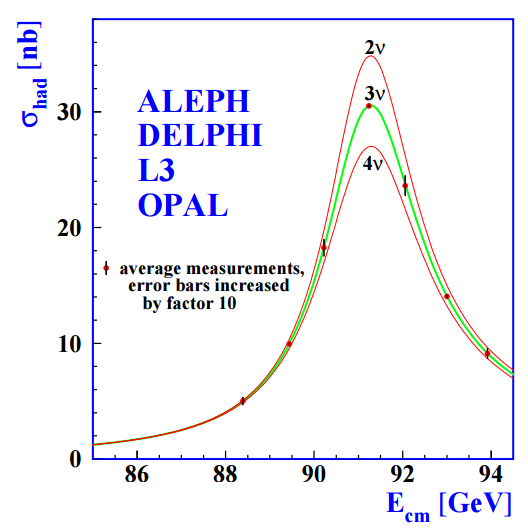
\includegraphics[width=90mm,scale=1.0]{figures/z.png} \caption{Data collected by ALEPH, DELPHI, L3 and OPAL experiments at LEP in CERN. The plot shows hadron production cross section around mass of Z boson as a function of LEP beam-energy, since  electron and positron can interact weakly the collision can product Z boson and we can measure width of uncertainty of mass of Z boson. Basically what we see in the figure as  hadron production cross section is Z boson creation cross section because in the experiment the hadrons are created by decay of the Z boson. Different curves show cross section predictions in case of 2, 3 and 4 standard neutrinos with negligible mass. \cite{LL}} \label{fig:z }\end{figure}  
%\\LEP measurements excluded existence of a fourth neutrino which is Z can decay into, so basically it means that there are just 3 standard neutrinos lighter than half of mass of Z boson.

In 1998 Super-Kamiokande (SK) detected an important lack in number of muon-type neutrinos that pass through the earth and reach the detector, moreover the deficit depended on energy and zenith angle \cite{vcx}. This is accepted as first evidence of neutrino oscillation, flavor change, which implies neutrino mass.

The tau neutrino was discovered at 2000 in FermiLab through Direct Observation of the Nu Tau (DONUT) experiment \cite{taud}.

Solution of the solar neutrino problem and confirmation of  $\nu$ oscillation came from SNO experiment in 2002 \cite{sno}. SNO was able to measure Charged Current (CC)   $\nu_{e} + d \to p + p + e^{-}$, Neutral Current (NC)   $\nu_{x} + d \to \nu_{x} + p + n$ and Elastic Scattering (ES)  $\nu_{x} + e^{-} \to \nu_{x} + e^{-}$, which explained Davis's missing  $\nu_{e}$, through  $\nu_{e} \to \nu_{\mu}$  or  $ \nu_{e} \to \nu_{\tau}$  oscillations.

Some of recent experiments on neutrinos are Daya Bay \cite{daya} and Reno \cite{reno} which are reactor beam based. One of the most important result of these experiment was to show that mixing angle  $\theta_{13}$ has a non-zero value which means it is possible to probe into CP violation in the lepton sector through the neutrino oscillation experiments. Their result was consistent with earlier T2K which is an accelerator beam based neutrino experiment \cite{T2K}. The value of the CP violation phase will be looking for the future experiments.
\\One of the future experiments is Deep Underground Neutrino Experiment (DUNE). It is a long base line tracking experiment which will include 2 TPCs \cite{dun}. The far detector will be at 1,475 m underground at the Sanford laboratory, the layer above the detector will be protection against cosmic background.
DUNE aims to measure the CP violation phase and determine the mass hierarchy of the neutrinos.

%These new experiments bring new limitations on neutrino-parameters which are can be found in the following chapter.

\subsection{Neutrino Theory}
Now according to Standard Model of Partycle Physics, there are 3 neutral neutrino partners to every charged lepton which are massless, have one half spin and only interact weakly. Neutrinos are left handed while their antiparticles are right handed.
However as demonstrated by SK and SNO, neutrinos oscillate between flavors, and which can be explained if neutrinos do have mass.

\subsubsection{Neutrino Oscillation}
Mass eigenstates of neutrinos do not coincide with their weak eigenstates. The mixing of the states is described as 
\begin{equation} \Ket {\nu_{\alpha}} = \sum_{i=1}^{3} U_{\alpha i}^{*} \ \Ket {\nu_{i}}  \ , \ \alpha=e, \mu, \tau  \end{equation}
where $\nu_{i}$ indicates mass states and $ U_{\alpha, i}$ is a $3 \times 3$ unitary mixing matrix which is known as ``Pontecorvo–Maki–Nakagawa–Sakata matrix" \cite{nost} and is presented as
\begin{equation} \begin{split}
U_{\alpha, i}
=
  \begin{pmatrix}
    c_{12} c_{13}& s_{12}c_{13} & s_{13} \ e^{-i \delta} \\
    -s_{12}c_{23}-c_{12}s_{23}s_{13}\ e^{i \delta} & c_{12}c_{23}-s_{12}s_{23}s_{13}\ e^{i \delta} & s_{23}c_{13}  \\
    s_{12}s_{23}-c_{12}c_{23}s_{13}\ e^{i \delta} & -c_{12}s_{23}-s_{12}c_{23}s_{13}\ e^{i \delta}  &c_{23}c_{13}
  \end{pmatrix} . \\ diag(e^{i \phi_{1}}, e^{i \phi_{2}}, 1 ) .\end{split} \end{equation}
The matrix consists of 3 mixing angles $\theta_{12}$, $\theta_{13}$, $\theta_{22}$ and 3 CP violating phases $\delta$, $\phi_{1}$, $\phi_{2}$, where $c_{ij}=cos \theta_{ij}$ and $s_{ij}=sin \theta_{ij}$. $\phi_{1}$ and $\phi_{2}$ are Majorana phases and they play role if the neutrinos are Majorana particles. As we will see in the following, neutrino oscillation probability is not depend on the Majorana phases, this means that the oscillations experiments cannot say anything about Majorana phases, the only way to work on Majorana phases is neutrinoless double-beta decay.
\\Consider an ultra-relativistic neutrino, evolution of the states between time $t=0$ and $t=t$ will be 
\begin{equation} \Ket {\nu_{\alpha}(t)} = \sum_{i=1}^{3} U_{\alpha i}^{*} \ \Ket {\nu_{i}(t)}.    \end{equation}
The probability of the oscillation from flavor $\alpha$ to $ \beta$ can be found via
\begin{equation}P_{\alpha \to \beta} = |\Braket{\nu_{\beta}(t)|\nu_{\alpha}}|^{2}.\end{equation}
Under a plane wave approximation, evolution of the states can be shown as
\begin{equation} \Ket {\nu_{\alpha}(t)} = e^{-iE_{i}t} \Ket {\nu_{\alpha}(0)}   , \end{equation}
where ultra-relativistic approximation allows us to express energy of the state as
\begin{equation} E = \sqrt{p^{2} + m_{i}^{2}} \approx p + \frac{m_{i}^{2}}{2E}  , \end{equation}
% via Maclaurin expansion
Via orthogonality condition $\braket{\nu_{\alpha}|\nu_{\beta}}=\delta_{\alpha  \beta}$, at the point we reached the oscillation probability is 
\begin{align*}  P_{\alpha \to \beta} = e^{-ip}  \sum_{i=1}^{3} \ U_{\alpha  i}^{*}\ e^{-i m_{i}^{2}/2p} \ U_{\beta  i}^{*}  \end{align*}
and this gives us
\begin{equation} \begin{split} P_{\alpha \to \beta} = \delta_{\alpha \beta} - 4 \  \sum_{i<j}^{3} Re (U_{\alpha  i}U_{\beta i}^{*}U_{\alpha  j}^{*}U_{\beta  j}) \ sin^{2}(\pi \frac{L}{L^{0}_{ij}}) \\  + 
2 \ \sum_{i<j}^{3} Im (U_{\alpha  i}U_{\beta i}^{*}U_{\alpha  j}^{*}U_{\beta  j}) \ sin^{2}(\pi \frac{L}{L^{0}_{ij}}),
\label{eq:lq} \end{split} \end{equation}
where \begin{equation}L^{0}_{ij} = \frac{4 \pi}{\Delta m_{ij}^{2}} \approx 2.48 \ \textrm{km} \ \frac{E(GeV)}{\Delta m_{ij}^{2} (eV^{2})} \ , \  \Delta m_{ij}^{2} =   m_{j}^{2} -  m_{i}^{2},  \end{equation} $L^{0}_{ij} $ is oscillation length in vacuum and $L$ is propagation distance of the neutrino. When $L << L^{0}_{ij} $ the oscillation probability is very small and when $L>> L^{0}_{ij}$ a lot of oscillations occur during the propagation, the optimal propagation distance is $L \approx L^{0}_{ij} $. At high energies L becomes very important, this explains observation of SK.
In Equation \ref{eq:lq} we see that if there were no difference between the masses or if $U$ was diagonal, there would be no oscillation, thus oscillation implies neutrinos have mass.
\\It is possible to write the mixing matrix as
\begin{equation} \begin{split}
U_{\alpha, i}
=
  \begin{pmatrix}
   1 & 0 & 0 \\
    0 &c_{12} & s_{12} \\
 0 & -s_{12} & c_{23}
  \end{pmatrix} 
  \begin{pmatrix}
   c_{13} & 0 & s_{13}\ e^{-i \delta}  \\
    0 & 1 & 0 \\
 -s_{13}\ e^{i \delta} & 0 & c_{13}
  \end{pmatrix} . \\
  \begin{pmatrix}
   c_{12}&s_{12} & 0 \\
    s_{12} & c_{12} & 0 \\
 0 & 0 & 1
  \end{pmatrix} diag(e^{i \phi_{1}}, e^{i \phi_{2}}, 1 ) .\end{split} \end{equation}
The first matrix can be tested via long baseline and atmospheric neutrino oscillations experiments.
The second one is again in the range of  long baseline oscillations experiments as well as reactor neutrino experiments. The third matrix can be tested via reactor and solar neutrino experiments. The diagonal part can be observed through neutrinoless beta decay. 
\\The second matrix has another importance as it includes a possible CP violating phase in the leptonic. This may be important to understand matter-antimatter imbalance in the universe. According to Sakarov conditions one needs CP violation in order to get more matter than antimatter \cite{sak}.
\\In matter, electron neutrinos feel an additional potential which changes effective mass of the neutrino and this affects on oscillation probability. This happens because while all neutrinos can interact with electron through neutral-current processes, only electron neutrinos interact with electrons via charged-current processes.
This phenomena is known as the ``MSW" or ``matter effect" \cite{nost}. 
%For 2 neutrino flavors, the oscillation probability is \begin{equation}P_{\nu_{e} \to \nu_{\mu}} = sin^{2}(2 \theta_{m}) \ sin^{2}( \frac{\Delta m^{2} L}{4 E}),\end{equation} where L is the length of the medium that is the neutrino propagated through, E is energy of neutrino, $\Delta m^{2}$ is effective mass-squared difference of the neutrinos and $\theta_{m}$ is mixing angle. This formula is not completely correct for our, known, 3 neutrinos-world but at least it is acceptable in short base line experiments where oscillation to tau neutrino does not play a big role. % it is also acceptable for atmospheric oscillations because L/E decreases effect of the electrons in that case.  \\There is a dependence of oscillation probability to L/E in all possible neutrino numbers and this dependence is the most important parameter of the experiments, 
%\\In the Equation \ref{eq:lq}, the first sinusoidal term behaves like an offset and by change the distance one can measure the offset and effect of the second sinusoidal term. (this was for 2 neutrino case)

\subsubsection{Masses of Neutrinos}

In the standard model there is nothing to explain the suppression of neutrino masses, which is 5 order of magnitude below the next lightest fermion. In Figure \ref{fig:sup} one can see comparison of the masses of quarks and leptons with possible neutrino masses.
\begin{figure}[h!] \centering 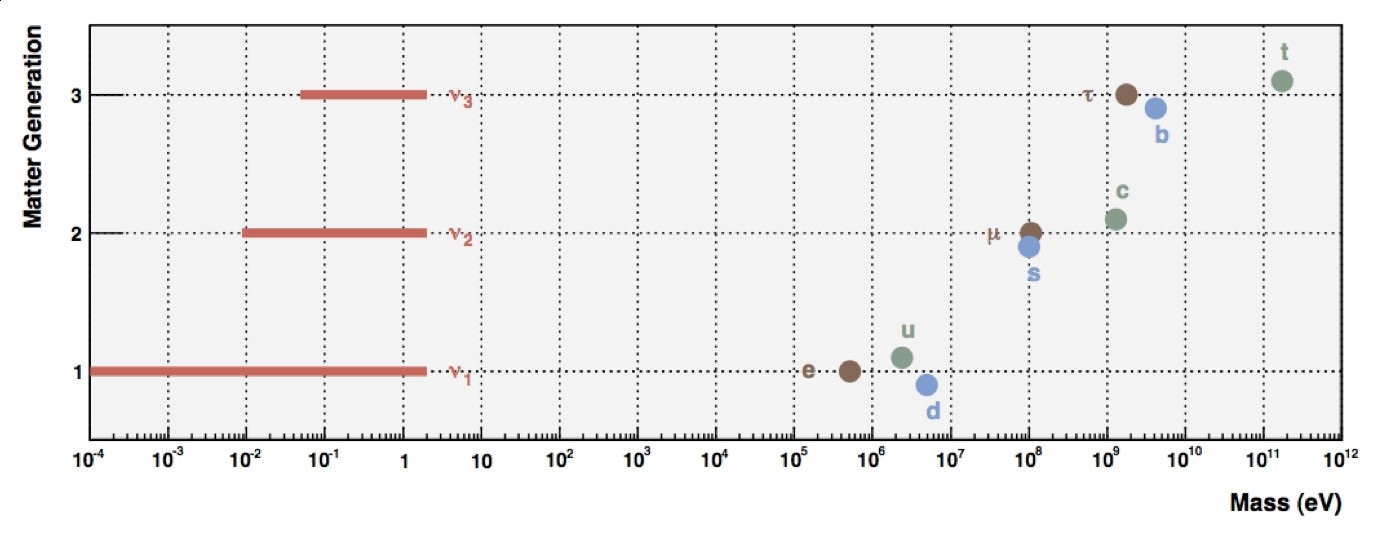
\includegraphics[width=120mm,scale=1.0]{figures/masses.jpg} \caption{Comparison of the masses of quarks and leptons with possible neutrino masses under normal hierarchy. \cite{masses}} \label{fig:sup} \end{figure}  %Dirac mass giving mechanism results too massive neutrinos, that is why in the SM we cannot explain.

The origin of the neutrino mass could be explained if neutrinos are shown to be Majorana particles, but as it is mentioned before the oscillation experiments are not sensitive to this.

Since Formula \ref{eq:lq} is proportional with effective mass-squared differences, experiments can only tell the magnitude of the mass differences of neutrinos. This situation leads to``mass hierarchy" problem, where we still do not know which one of the mass eigenvalues are bigger or smaller than the others. There are two conventionally-considered scenarios;
\begin{align*}
Normal \ hierarchy : m_{3} > m_{2} > m_{1}  \\ 
Converted \ hierarchy : m_{2} > m_{1} > m_{3}  
\end{align*}

\begin{figure}[h!] \centering 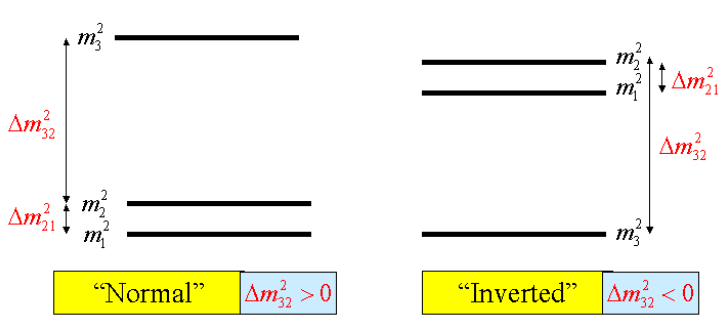
\includegraphics[width=110mm,scale=1.0]{figures/mass.png} \caption{Normal and converted mass hierarchy scenarios. \cite{massr}} \end{figure}  

\end{comment} %1

\begin{comment}
James told that I should not put this part in the thesis.
Another possible scenario about to order mass squares is quasi-degenerate masses which is possible both for normal and converted hierarchies \cite{conm};

\begin{align*}
Normal \ hierarchy : m_{\nu}^{QD} \simeq m_{3} \gtrsim m_{2} \gtrsim m_{1}  \\ 
Converted \ hierarchy : m_{\nu}^{QD} \simeq  m_{2} \gtrsim m_{1} \gtrsim m_{3}  
\end{align*}
with
\begin{equation}m_{\nu}^{QD}  \gg \sqrt{\Delta m_{A}^{2}} \approx 5.10^{-2} \ eV ,\end{equation}
where
$\Delta m_{A}^{2} = \frac{1}{2}  \abs{\Delta m_{12}^{2} + \Delta m_{23}^{2}}$.

Because of lepton number conservation, we think that neutrino and anti-neutrinos are different particles but it is still not proven that they may not be the same particle. Complex conjugation of a particle's wave function gives wave function of its anti-particle, if the wave function is real then the particle is its own anti-particle, this kind of particles are known as Majorana particles. 
\\As it is mentioned before, in the Standard Model (SM), neutrinos do not have mass and this fixes their handness. Also in the SM, left handed particles and right handed anti-particles can interact weakly. Since the neutrinos have mass, it is possible that actually neutrino and anti-neutrino are the same particle, left handed neutrinos interacts as neutrino, right handed neutrinos interact as anti-neutrino, this kind of neutrino is called ``Majorana Neutrino" and we still do not know if this is the case in the real life.
\\Double beta decay can help us to understand if the neutrinos are Majorana, if neutrinos are Majorana particles, it would be possible to observe a neutrino-less double beta decay. The problem about the double beta decay; it occurs very rare and this makes difficult to get reliable experimental results.

% By observing the gamma created in this annihilation could also help us to understand mass of the neutrinos : FOR HERE IGOR SAID THAT in neutrinoless one, the neutrinos are virtual and we cannot say that they "annihilate", neutrinoless has a sharp energy spectrum.

%in this decay the nucleus emits 2 electrons and 2 neutrinos, if the neutrino is its own anti-particle, it is possible that these 2 neutrinos can make annihilation, this kind of decay is known as "neutrino-less double beta decay". 
\end{comment}

\begin{comment} %2
Future oscillation experiments, such as DUNE, will attempt to measure the hierarchy through observations of $\delta^{CP}$, which is degenerate in different hierarchies \cite{mcp}

Some experiments, like MiniBooNE, brought the idea of ``sterile neutrino", that only interacted with gravity and not weak force.
Note that there is no physical reason to limit the number of mass eigenstates to 3, this means that neutrinos could oscillate into a sterile state.
\end{comment} %2

\begin{comment}
There are 2 types of sterile neutrinos proposed;
\begin{enumerate}
\item  Through see saw mechanism-is very heavy RH- not detectable at low energy
\item Extra mass eigen state-what miniboone look for
(James said just know this, do not put in the thesis)
\end{enumerate}
\end{comment}


%Sterile neutrino is a kind of neutrino which interacts just via gravitation, standard weak interaction says that just left handed neutrinos can weakly interact, for example if there is a right handed neutrino it would be a sterile neutrino. james said that this would be Majorana, not light sterile. 
\begin{comment} %3
\subsection{Interactions of Neutrino and Neutrino Experiments}
Neutrinos can interact via CC and NC weak interactions. Mediators of the CC are $W^{+ / -}$ bosons and the mediator of the NC is the $Z^{0}$ boson. 
Low energetic neutrinos can make only NC interactions while high energetic neutrinos can make both neutral and charged current interactions, because in the second one the neutrino transforms into its charged lepton partner. NC interactions are more possible with quarks than electrons, we see this interaction as production of meson or baryon, one can see the Feynman diagrams of some possible interactions in Figure \ref{fig:nccc}. 
\begin{figure}[h!] \centering 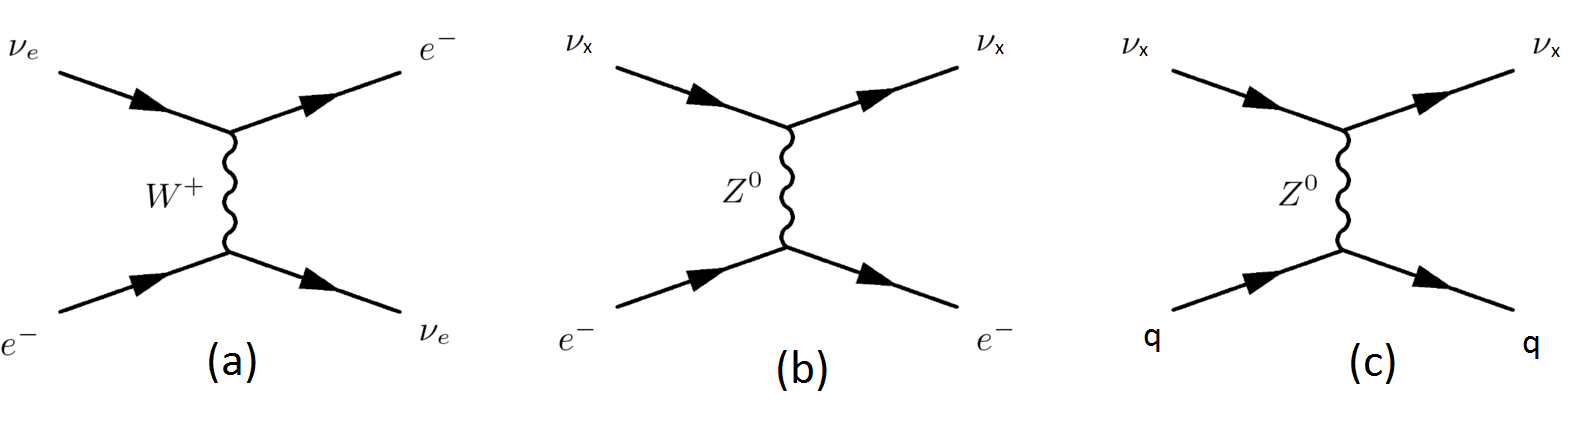
\includegraphics[width=100mm,scale=1.0]{figures/nccc.png} \caption{(a) CC interaction of electron neutrino via $W^{+ }$ boson. (b) NC interaction of a neutrino, this interaction is possible for all kind of neutrinos while (a) is possible just for electron neutrinos. In the detector, (a) and (b) are not distinguishable. (c) In the substance, the NC interaction is more possible with quarks than electrons, we see this interaction as production of meson or baryon.}\label{fig:nccc} \end{figure}  
At energies lower than 1 GeV NC interactions are dominated while for higher energies the CC \cite{askthissource}.

The interaction types of neutrinos determine the design of neutrino detectors. An advantage of CC is that it allows to determine the flavor of the neutrino by observing the charged lepton partner. NC interactions are detected when the transferred energy and momentum break the target nucleus or an electron from the target atom. 
For example, the energy needed to produce an ion par in LAr is 23.6 eV, and the energy needed to produce scintillation light is 19.5 eV, so even a low energetic neutrino is able to create ionization or scintillation in LAr.

There are 2 basic examination principles of neutrino oscillation experiments; look for appearance and disappearance of a flavor type. 
In appearance measurements, one starts with a certain amount of a type of neutrino and at a determined distance the amount of an other type of neutrino is measured. 
In the disappearance experiments, again one starts with a certain amount of a type of neutrino and at a determined distance the amount of the same type of neutrino is measured.

The experiment method used in SBN project is tracking and the source of the neutrinos is accelerator based. Before starting to discuss on the tracking experiments, neutrino production procedure will be presented.

\subsubsection{Accelerator Neutrinos}
\label{chap:an}

Production starts with acceleration of protons. The protons are accelerated in a synchotron, % synchotron is a diferent version of cyclotron which is magnetic filed is time depended and SYNChronized to kinetic energy of the particle. 
their energy determine energy of the final product, the neutrinos. After the protons reach to desired energy, they are directed on a target to produce some hadrons.
\\A focusing horn surrounds the target and focuses the produced particles with a magnetic field, which also helps choose the charge of the hadrons. Focused hadrons propagate through ``decay volume" where they decay and produce other particles. The majority of the particles created in the interaction of protons with the target are pions and they decay as $\pi^{+} \to \mu^{+} +  \nu_{\mu}$.
\\There are other sources of neutrino from the beam, muons created here may decay as $\mu^{+} \to \bar{\nu}_{\mu} +  e^{-}$ + $\bar{\nu}_{e}$. 
Second, hadronic interaction of protons with the target also produces kaons. Kaons can decay as  $K^{+} \to \mu^{+} + \nu_{\mu}$,  $K^{+} \to \pi^{0} + e^{+} + \nu_{e}$ and $K^{+} \to \pi^{0} + \mu^{+} + \nu_{\mu}$.
The mean life time of kaon is $\tau_{kaon}=12 \ ns $, and $\tau_{pion}=26 \ ns $ and $\tau_{muon}=2.2 \ \mu s $. The length of the decay volume is chosen in a way that pions have enough time to decay to produce muons and muon neutrinos but only a small percentage of the muons can decay.
In this time kaons will also decay and produce a neutrinos.
At the end of the decay volume there is an absorber which absorbs the particles except neutrinos, though a small amount of the muons can pass the absorber and be used monitor the particle flux.
\end{comment} %3
\begin{comment}
(James did not want me to put here)
The same neutrino production process also happens in the atmosphere. Earth's atmosphere is under bombardment of cosmic particles, 90 \% of these particles are protons and 9 \% are alphas. Interaction of high energetic protons create pion shower which lead to muon neutrinos. Atmospheric neutrinos have a very wide range of energy because of the energy of incoming protons.
\\Natural neutrino sources are good information mediators of some of natural events like energy creation by fusion in Sun or supernovas \cite{spn}.
\\In the sun there is a long process about energy production which is known as ``pp-chain". Solar neutrinos are electron neutrinos, big percentage of them are created at the beginning of pp-chain while producing Deuterium, and have energy $<0.42$ MeV. Another important source of neutrino in the space is supernovas, supernovas release a significant amount of their energy in form of electron neutrino.

If one continuously keeps the muons in an accelerator, accelerator rises the life time of the muons respect to laboratory-observer, thus we can control decay of the muons and use it for our purposes. This method is known as ``neutrino factory".

Beta decay is the most often used nuclear interaction of the neutrino and produces pure neutrino beams. 
In fission reactors, the unstable atoms decay through inverse beta decay to a stable state and this results creation of anti-neutrinos. These neutrinos have low energy, about several MeV.
\\If one wants hight energetic neutrinos from beta decay, one can ionize and accelerate the unstable nuclei before it decays, this increase energy of the neutrino.
\end{comment}

\begin{comment} %4
\subsubsection{Tracking Experiments}

Observing particles via tracks is one of the popular methods which is used also in SBN program. Here, information of the interaction is obtained by reconstructing the ionization tracks.
\\It is possible to perform tracking experiments in 2 ways; one can collect the charge produced by ionization, as in liquid Argon (LAr) Time Projection Chambers (TPCs), or one can observe track of ionization, as in emulsion films.
A magnetic field applied to ionization medium can allow to directly observe sign of charge of the incoming particle and calculate the particle's momentum.

Tracking experiments have higher energy threshold than the other methods because for a good reconstruction we need strong ionizations, that is why they are generally suitable for high energetic neutrinos.%how much high?

In the charge-collection method, the medium can be liquid or gas and the charge is collected via an electric filed. An advantage of the liquid medium; it is denser and for particles which have low cross section, like neutrino, this is better, advantage of the gas medium; here just photons can create shower because of the low intensity.
Solid medium is good for short living particles like tau, one of the experiments which use this method is OPERA (Oscillation Project with Emulsion tRacking Apparatus).
\end{comment} %4
\begin{comment}

(James did not want)
\subsubsection{Cherenkov Experiments}

In a transparent medium, when a charged particle moves faster than speed of light, it emits radiation which is known as Chereknov radiation. The emitted radiation has shape of a cone, direction of the cone is related with moving direction of the particle and opening angle of the cone is a function of the velocity of the particle, see Figure \ref{fig:che }.
\begin{figure}[h!] \centering 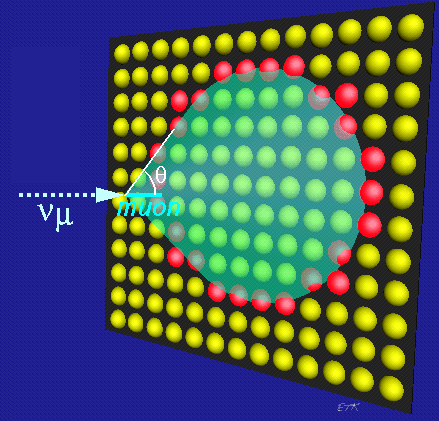
\includegraphics[width=100mm,scale=1.0]{figures/che.png} \caption{ Emitted radiation has shape of a cone, direction of the cone is related with moving direction of the particle and opening angle of the cone is a function of the velocity of the particle. It is possible to detect this radiation by Photomultipliers. Adopted from \cite{N}} \label{fig:che } \end{figure}  

Energy loss through Cherenkov radiation is very small compared to ionization, that is why the Photomultipliers (PMTs) which will collect the radiation should be very sensitive.
Cherenkov detectors are not every time good for particle identification, for example they cannot distinguish between muon and pion, but it is possible to distinguish between electron and muon by looking at the shape of the radiation rings, see figure \ref{fig:cri }.
\\LSND and MiniBooNE experiments, which are will be discussed with more detail in Chapter ?, took help from Cherenkov radiation in order to determine the interactions, but since the Cherenkov detectors are not able to distinguish between photons and electrons, they left a mystery behind them related with oscillation of electron kind of neutrinos.
\begin{figure}[h!] \centering 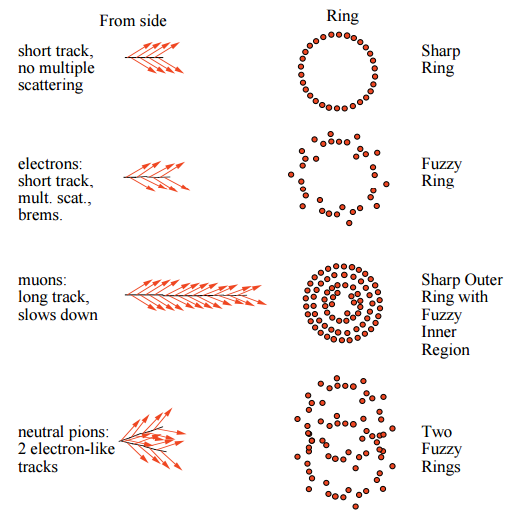
\includegraphics[width=100mm,scale=1.0]{figures/cri.png} \caption{Illustration of Cherenkov rings in the MiniBooNE. For CC interactions MiniBooNE can be seen as Cherenkov detector \cite{KN}.}\label{fig:cri } \end{figure}  

Water Cherenkovs are more sensitive to electron neutrinos, this is not just because of electron's CC advantage, but also for electrons threshold kinetic energy to emit Cherenkov radiation is lower than muons and taus, we can order the threshold energies as $E^{th}_{e} < E^{th}_{\mu} < E^{th}_{\tau}  $, also to create electromagnetic shower is much easier for electrons.

As it is mentioned before, one of the famous Cherenkov detectors is SK \cite{zukf}. Cherenkov detectors are not just liquid-environment detectors, detectors like IceCube \cite{icec} use natural ice in the poles as detection environment and detect the Cherenkov radiation by PMTs located in the ice.
\\Heavy-water Cherenkov detector is another possibility, since Deuterium has a very low binding energy, 2.2 MeV, to break it is very easy, by observing the broken Deuteriums, one can have information about NC and CC interaction in the detector, more precisely, after interaction of neutrino and heavy water, if we have two protons and one electron, this is a CC, if we have one proton, one neutron and one neutrino which is we don't see, this is a NC interaction. Sudbury Neutrino Observatory \cite{sno} was one of the heavy-water Cherenkov detectors.

\subsubsection{Scintillation Experiments}
Inverse beta decay, $p^{+} + \bar{\nu}_{e} \to  + e^{+} + n^{0} $, is one of the most important neutrino interactions that it is also base of scintillation experiments. Scintillation detectors use liquid scintillator as detection environment, after the inverse beta decay, in several $\mu s$ the positron will be captured by electrons in the medium and this will produce gamma ray pairs. The neutron will be captured by an atom rather slowly, can be hundreds of  $\mu s$, more precisely it is depend on the elements in the medium, in order to make this capture quicker, generally a material which has high neutron affinity, like cadmium, is added. Capture of the neutron creates a gamma, if one knows the expected time difference between fast and slow signals, this can be used to avoid background.
\\As it is mentioned before, scintillation experiment-method has a historical importance because, the first neutrino, electron neutrino, discovered through this method.
Scintillation detectors have good energy resolution but cannot give directional information of the event like Cherenkov detectors.
\\One of the scintillation experiments is MiniBooNE, which includes 800 tons scintillating mineral oil and 1200 PMTs to detect scintillation light.

\subsubsection{Radiochemical Experiments}
Here, again the basic interaction is inverse beta decay, the biggest advantage of this method is its threshold, it has the lowest energy threshold among the methods. 
\\In this kind of detection, neutrino is absorbed by an atom and after the inverse beta decay a radioactive isotope is produced, one can get number of the neutrino interactions by observing number of these isotopes.

Gallex experiment is a radiochemical experiment which has a very low energy threshold;  233.2 keV. The base reaction of the experiment is $^{71}Ga + \nu_{e} \to ^{71}Ge  + e^{-}  $, 

\subsubsection{Future Experiments}

dune cut


Hyper-Kamiokande is a next generation underground water Cherenkov detector, its total mass is about 25 times bigger than SK's and has higher sensitivity than SK \cite{hypk}. It aims to take measurements on the neutrino oscillation and CP violation in lepton sector.

Cryogenic Low-Energy Astrophysics with Neon (CLEAN) is a future scintillation experiment which will be able to look for interactions of very low energetic neutrinos and the other weakly interacting particles \cite{clle}. 

\end{comment} 

%%%%%%%%%%%%%%%%%%%%%%%%%%%%%%%%%%%%%%%%%%%%%%%%%%%%%
\clearpage

\section{Short-Baseline Neutrino Program}
\label{chap:sbnp}

The Short-Baseline Neutrino (SBN) Program is located at FermiLab, near Chicago, and is searching for neutrino oscillations at an L/E around 1 km/GeV. Hints of oscillation at this L/E value were seen by LSND and MiniBooNE experiments.

SBN is an accelerator-based neutrino beam program and includes three LArTPCs to perform $ \nu_{e}$ appearance and  $ \nu_{\mu}$ disapearance measurements. The neutrino beam used here is known as the Booster Neutrino Beam (BNB) which has energy around 800 MeV. BNB will be described later with more details.
\\Accelerator-based neutrino beam experiments benefit from a near detector in order to characterize the beam and a far detector to be able to perform oscillation experiments. In the SBN program the near detector is the Short Baseline Near Detector (SBND) which is located at 110 m from the BNB target \cite{prop}. SBN will have two far detectors: at 470 m from the BNB target MicroBooNE, and at 600 m ICARUS, the former is already running.

To understand the goals of the SBN program better, its motivations will be discussed in the following section.

\subsection{Motivation of Short-Baseline Neutrino Program Program}

The biggest motivations of the SBN program come from Liquid Scintillator Neutrino Detector (LSND) and from the MiniBooNE experiments.
\\LSND was a short-baseline liquid scintillator detector which was built to detect neutrino oscillation and operated from 1993 to 1998. It used neutrinos from pion decay at rest and detected scintillation light as well as Cherenkov radiation. LSND's results showed an excess of electron anti-neutrino events in the region of L/E=0.4 to 1.2 (km/GeV) \cite{K}, % which can be interpreted as $\bar{\nu}_{\mu} \to  \nu_{sterile}  \to  \ \bar{\nu}_{e}$ oscillation. 
see Figure \ref{fig:lsnd}.
\begin{figure}[h!] \centering 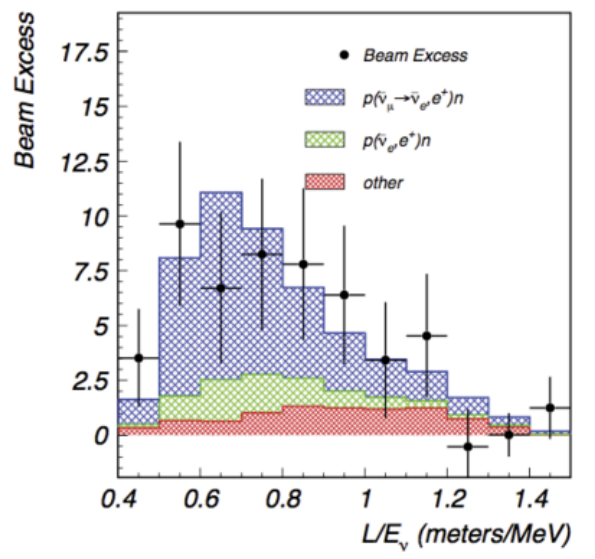
\includegraphics[width=70mm,scale=1.0]{figures/lsnd.png} \caption{Observed $\bar{\nu}_{e}$ data in the LSND experiment are the black dots. Red and green areas are backgrounds and blue area is the best fit to $\bar{\nu}_{\mu} \to  \bar{\nu}_{e}$ neutrino oscillation signal. \cite{MN}} \label{fig:lsnd} \end{figure}  
\\MiniBooNE was a follow-up experiment designed to test the LSND oscillation hypothesis.
%It includes 800 tons scintillating liquid. 
It is a Cherenkov detector which is located in FermiLab. It used pion decay in flight neutrinos,
while the energy of the neutrino flux in LSND was 20 to 53 MeV, the average energy of the flux in MiniBooNE was 800 MeV.
MiniBooNE observed an excess of $\nu_{e}$ and  $\bar{\nu}_{e}$ events particularly at neutrino energies lower than 475 MeV.
The distribution of electron anti-neutrino and electron neutrino oscillation candidates from MiniBooNE and the expected backgrounds can be seen in Figure \ref{fig:ndata}. 
\begin{figure}[h!] \centering 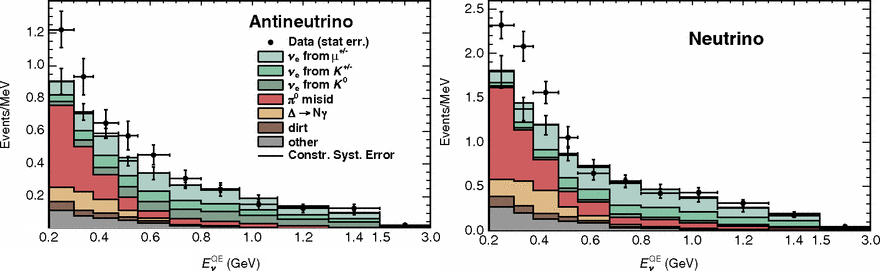
\includegraphics[width=124mm,scale=1.0]{figures/ndata.png} \caption{Distribution of electron anti-neutrino (left) and electron neutrino (right) oscillation candidates from MiniBooNE \cite{KP}. In the graphs one can see the expected distribution of background and data from the experiment. The energy cut-off is at 200 MeV, because below this value background is very high.} \label{fig:ndata}\end{figure}  
%Why do not we try to explain the signal excess, for example in MiniBooNE, with a neutrino heavier than Z boson but we produce a new kind of neutrino? Because a neutrino more massive than Z boson cannot create that kind of signal, there  $\Delta m^{2}$ is $\approx 1$, with a new neutrino is heavy, the standard ones have to be also heavy which does not match with the experiments. WORK WITH HERE
\\Cherenkov detectors have difficulty in distinguishing electrons from photons since both of them create electromagnetic shower.
The electron neutrino excesses which were observed both at LSND and MiniBooNE could be misidentification of photons originated from unknown sources.
%, for example the photons originated from an unexpected nuclear excitation .excitation of nucleus or decay of $\pi^{0}$. 
LSND and MiniBooNE left a mystery behind them which could be a hint of new physics. %hint of sterile neutrinos.
\\The SBN program will investigate the excess of signal seen in both LSND and MiniBooNe through LArTPCs.

LArTPCs are able to distinguish electrons from photons by looking at the beginning of the showers. A simulation can help to understand this fact, shown in Figure \ref{fig:epi}. In the figure, on the left, we see a shower created by an 1 GeV electron, and on the right we see 2 showers created by 2 photons that are originate from decay of an 1 GeV $\pi^{0}$. 
The energy deposition at the beginning of the shower induced by the electron is lower than at the beginning of the photon showers because, due to $e^{+}$  $e^{-}$ pair production of the photon, the latter one has 2 ionizing particles, see Figure \ref{fig:mic}.
\begin{figure}[h!] \centering 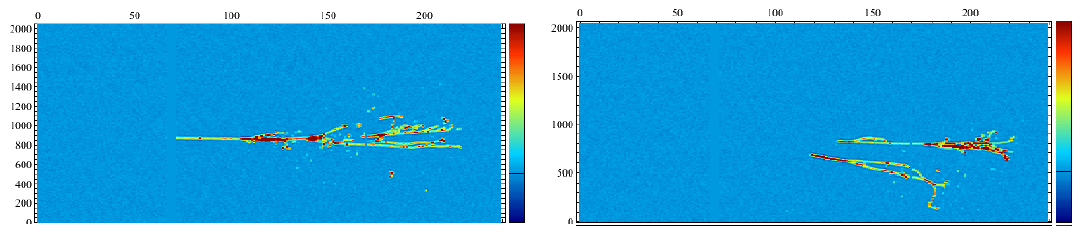
\includegraphics[width=124mm,scale=1.0]{figures/epi.png} \caption{Simulations of electromagnetic showers in a LArTPC. On the left, we see tracks created by a 1 GeV electron, and on the right we see track of 2 showers created by 2 photons that are originate from decay of a 1 GeV $\pi^{0}$. Unlike the photon, the electron leaves a nice track behind it before the shower starts. The vertical axis is the hit time of the collected charge to the collection wires and the horizontal axis is the channel number on the collection wire plane \cite{LK}.} \label{fig:epi} \end{figure}  
\begin{figure}[h!] \centering 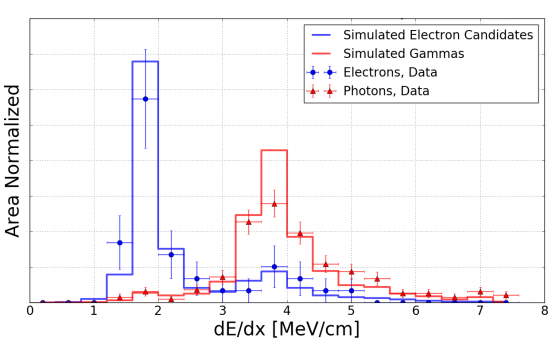
\includegraphics[width=124mm,scale=1.0]{figures/mic_neu.png} \caption{Energy deposition simulations and measurements for electrons and gammas in the ArgoNeuT LArTPC. By observing energy deposition at the beginning of a shower one can distinguish between photons and electrons. At the beginning, energy deposition of the photon's shower is about 2 times bigger than electron's shower. \cite{mic}} \label{fig:mic}\end{figure}  
%\\Since the SBN program will be sensitive in the $\Delta m^{2} \approx 1 eV^{2}$ region, it will be able to deal also with "reactor neutrino anomaly" [PK] which means anomaly in $\bar{\nu}_{e}$ disappearance measurements performed by using reactor neutrinos.

%The most preferred noble liquid to fill inside TPCs is argon, because it is relatively inexpensive, has high density that is good to get a higher interaction rate, has high ionization yield because of its low ionization energy (in average 23.6 eV is needed to ionize an electron from LAr) which gives better ionization tracks, and it is highly transparent to its scintillation light.

The intermediate LArTPC in the SBN program is MicroBooNE which was built to test the existence of the signal excess reported by MiniBooNE and measure the LAr-neutrino interaction cross sections. 
%But still position of $\mu BooNE$ is set in a way that it will also help for the oscillation experiments in the program. The positions are chosen in a way that measurement on oscillation probability is optimized and effect of systematic errors is minimized. 
\begin{comment}
In Figure \ref{fig:3tenors} one can see the different oscillation probabilities for 3 detectors calculated for 3 standard + 1 sterile neutrino fit based on LSND data. \begin{figure}[h!] \centering 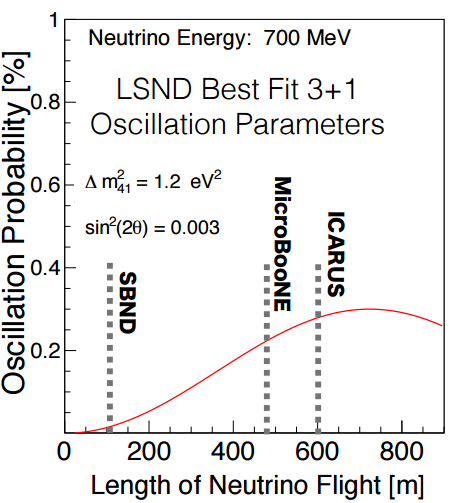
\includegraphics[width=100mm,scale=1.0]{figures/3tenors.png} \caption{Here one can see where the detectors reside respect to oscillation probability calculated from 3 standard + 1  sterile neutrino fit based on LSND data \cite{MNR}.  } \label{fig:3tenors} \end{figure}  
\end{comment}
In the following, after the neutrino beam production in the SBN program, MicroBooNE is presented.

%Solar and reactor neutrinos have enough energy to make NC interactions, CC is possible only for electron neutrino.
%Critical energy for electron in LAr is 30 MeV.

\subsection{Neutrino Production}
In the SBN project the neutrinos are produced in pion decay in flight. The pions are created in the collision of protons with a target.
Before the collision the protons are accelerated in a synchotron, % synchotron is a diferent version of cyclotron which is magnetic filed is time depended and SYNChronized to kinetic energy of the particle. 
their energy determine energy of the final product, the neutrinos.% After the protons reach the desired energy, they are directed on a target to produce pions.
\\A focusing magnetic horn surrounds the target and focuses the produced charged particles, which also allows to choose the charge of the pions. The focused particles propagate through 50 m long ``decay volume". 
The majority of the particles created in the interaction of protons with the target are pions and they decay as $\pi^{+} \to \mu^{+} +  \nu_{\mu}$. The length of the decay volume is chosen in a way that pions have enough time to decay to produce muons and muon neutrinos.
There are other sources of neutrino from the beam, the muons created here may decay as $\mu^{+} \to \bar{\nu}_{\mu} +  e^{-}$ + $\bar{\nu}_{e}$. 
Second, hadronic interaction of protons with the target produces also kaons. 
In the decay volume also the kaons will decay and produce neutrinos.
\\At the end of the decay volume there is an absorber which absorbs the particles except neutrinos. A small amount of the muons also can pass though the absorber which could be used to monitor the particle flux.
\begin{comment}
The neutrino beam production starts with hydrogen plasma. To get protons a tandem accelerator is used. %this also provides primarily acceleration
The plasma is accelerated in the first part of the tandem accelerator where $H^{+}$ is collected and just $H^{-}$ is accelerated. $H^{-}$ is chosen to be accelerated because the creation of $H^{-}$ needs lower energy than $H^{+}$. At the end of the acceleration medium there is a carbon foil which strip off the electrons of $H^{-}$ as it passes through. In the second part of the accelerator, the protons are again accelerated.

\\The main accelerator used in this project is called ``Booster" which is a 474 meter-circumference synchrotron. The Booster receives 400 MeV protons from a Linear Accelerator (Linac) and outputs 8 GeV protons.
Accelerated protons are directed into a 5 mm wide and  71 cm long Beryllium target and produce secondary hadrons. 

The target has an air-cooling system, this is needed because the protons dissipate 600J per second in the target \cite{PR}. The main products of the interaction between the target and protons are pions which decay as $\pi^{+} \to \mu^{+} +  \nu_{\mu}$.

Using a focusing magnet (also called focusing horn),% which can be seen in Figure \ref{fig:horn}, 
the secondary hadrons are directed to a decay volume. They propagate through this 50 m air-filled tunnel where they decay. %The decay tunnel contains air, the air is there since it is difficult to evacuate but this does not create a problem. 
\\At the end of the decay volume a roughly cubic, 3 m on side, steel absorber absorbs the surviving particles, except neutrinos.
It is possible to change polarity of the horn, this allows us to make a choice between neutrino and anti-neutrino beams.
\begin{figure}[h!] \centering 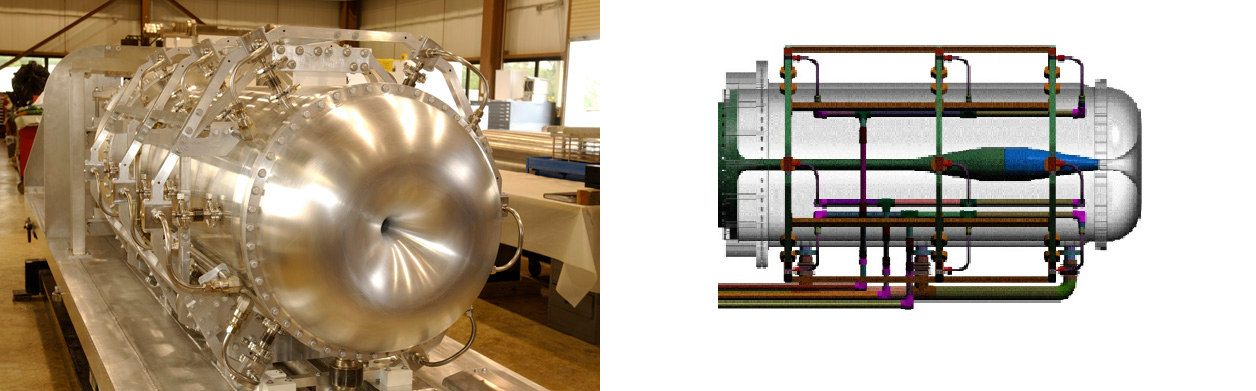
\includegraphics[width=120mm,scale=1.0]{figures/horn.png} \caption{Left, photo of focusing horn of Booster accelerator, it focuses the secondary hadronic beam \cite{KM}. Right, transparent drawing of the horn with its water cooling system. Here the beam direction is from left to right \cite{PR}.}\label{fig:horn} \end{figure} 

\end{comment}

In this way a neutrino beam which is 1.6 $\mu$s long and has a repetition rate of 5Hz is produced. The average neutrino energy is 800 MeV.

\subsection{MicroBooNE}

MicroBooNE is a LArTPC which has 10.4~m~(length)~$\times$ 2.5~m~(width) $\times$ 2.3~m~(height) active volume. It is located at FermiLab. Figure~\ref{fig:mb} shows a drawing of MicroBooNE with its components and Figure~\ref{fig:mbtpc} illustrates its TPC.
The boiling point of Ar is at 87 K, therefore cryogenic equipment is necessary to operate LArTPCs. In MicroBooNE, the detector sits in a cylindrical stainless cryostat. To achieve a high signal to noise ratio, custom pre-amplifiers which operate at liquid argon temperatures were developed. The equivalent noise in MicroBooNE is below 1000 $e^{-}$ per wire. %this is only electronic noise
\begin{figure}[h!] \centering 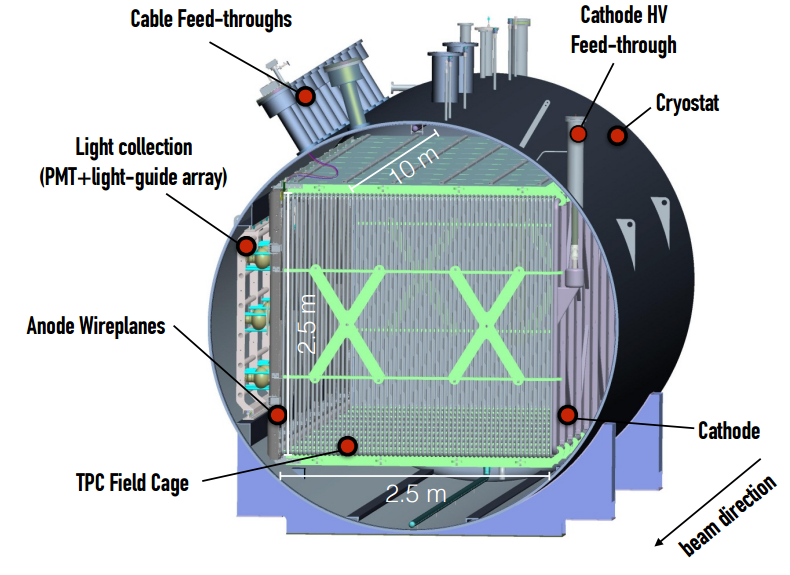
\includegraphics[width=120mm,scale=1.0]{figures/mb.png} \caption{A drawing of MicroBooNE with its components. It has 10.4 m (length) $\times$ 2.5 m (width) $\times$ 2.3 m (height) active volume. \cite{PP}.} \label{fig:mb}\end{figure}  

Ionization electrons created by an ionizing particle in the active volume of the TPC are drifted toward the anode via the electric field which originates from a large negative potential applied by a stainless steel cathode.
In order to get an uniform electric field, a field cage decreases the applied voltage step by step from anode to cathode. Basically the field cage consists of parallel metallic tubes which have resistors between each of them, this structure provides also mechanical strength for the TPC.
\\The size of the anode in MicroBooNE is 10 m x 2.3 m and consists of 3 wire-planes: the Y, U and V planes contain 3456, 2400 and 2400 gold-plated stainless steel wires, respectively. In Figure \ref{fig:mbtpc}, U is the fist wire-plane seen by drifting electrons, followed by V and than Y. The Y plane has vertically-oriented wires, while the U and V planes are oriented a $+/- \ 60^{o}$.
Both the wire pitch and the distance between the wire planes is $\approx 3~mm$.
%, this means coordinate resolution in the TPC is 3 mm. 
%At the beginning, the electric field between cathode and anode was planned to be 500 V/cm, for 2.5 m this results in -125 kV cathode voltage, but till now the maximum electric field we reached is $\approx$ 273 V/cm. 
The current electric field in the TPC is $\approx$ 273 V/cm. 
For the calibration of this electric field MicroBooNE uses a novel UV laser system \cite{prop}.
%, makes $\approx$-70 kV bias.
\\The 2 dimensional position information of the tracks, let us say z and y coordinates, come from the wire planes while third coordinate, x, comes from drift time. In order to determine the drift time, one needs to know the interaction time which one gets from Photomultipliers (PMTs) in the cryostat. These PMTs detect the scintillation light created in an interaction of an incoming particle with LAr. 
The drift time which is obtained from here is the time difference between the signal in the PMTs and anode wires.
\begin{figure}[h!] \centering 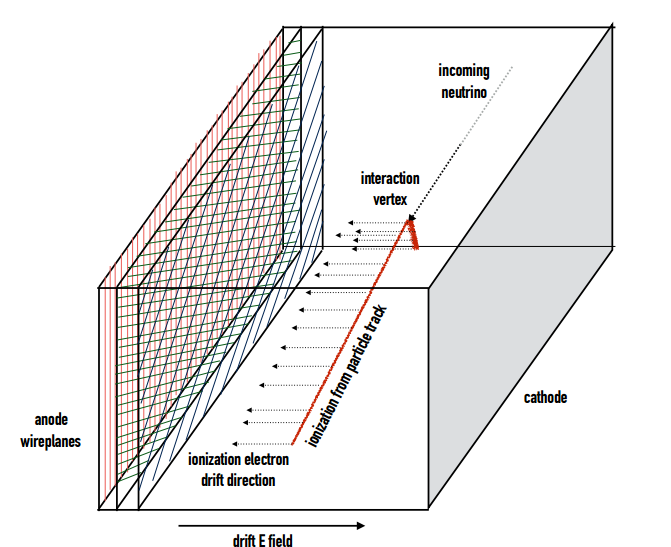
\includegraphics[width=120mm,scale=1.0]{figures/mbtpc.png} \caption{A drawing of the TPC of MicroBooNE. The electric field leads to collection of the ionization charge, 2D position information of the tracks, let us say z and y coordinates, come from the wires, the third coordinate, y, comes from drift time. \cite{PP}} \label{fig:mbtpc}\end{figure}  

\begin{comment}
Ar has an emission peak at 128 nm, and LAr scintillation light can be produced in 2 ways which are illustrated in Figure \ref{fig:argo}.
One of the ways is the excitation of Ar atom by an incoming particle and the excited Ar atom traps a second Ar atom and forms excited $\textrm{Ar}_{2}$. The excited molecule emits scintillation light when it falls back into the ground state.
The other way is after ionization of the Ar atom. The ionized Ar atom has a high electron affinity and it forms a bound state with another Ar atom to create an ionized molecule. After a while, this molecule absorbs a free electron from the medium and becomes a neutral excited molecule, after emission of scintillation light the atoms leave each other. Since this process needs an external electron, the amount of the scintillation light emitted through this process is depend on the recombination factor which is a function of electric field.
\\As we see both of the ways includes an excimer Argon and its decay produces the scintillation light. The speed of the scintillation light is depend on how the spin of the electron and argon dimer combined. Here a single state or a triplet state is possible, and emission of the single state is faster than the triplet state. Fast emission has a life time of about 6 ns while in the pure Ar slow emission needs about 1500 ns. Emission through triplet state is depend on the purity of the Argon, such that this emission time can be used as a measure of the purity \cite{sint}.

\begin{figure}[h!] \centering 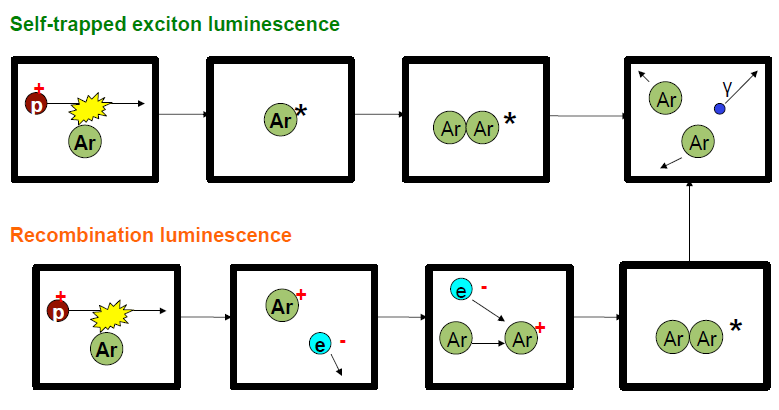
\includegraphics[width=110mm,scale=1.0]{figures/argo.png} \caption{In LAr scintillation light can be produced with 2 ways; excitation and ionization of the Argon. \cite{MP}} \label{fig:argo} \end{figure}  

Scintillation light can be used in LArTPC also in several ways; % \cite{R}:
\begin{itemize}
\item To tagger neutrino interactions. Here the scintillation light should appear in $1.6~\mu~s$ beam spill. At the beginning the primary importance of the optical system was to trigger the TPC, since prompt scintillation light is much faster than the drift time this is possible, but now the tracking is made by BNB.
%to avoid background neutrinos and cosmic rays. If these backgrounds do not come in time window of BNB, $1.6 \ \mu s$, timing of the scintillation light can help to avoid them.
\item To help determine the energy released in the Ar by ionizing particles; and
\item To help determine the identity of the particles via the shape of the scintillating light.
\end{itemize}
%time difference between slow and fast times can be used for background elimintaion right?
MicroBooNE has 32 Hammamatsu R5912-02mod 8 inch cryogenic PMTs to detect the scintillation light. %see Figure \ref{fig:pmmb}.
\\Scintillation light yield for a Minimum Ionizing Particle (MIP) in MicroBooNE is $\approx$ 40000 photons/MeV. The presence of the electric field decreases the amount of observable photons by the PMTs. 
At the moment MicroBooNE applies a threshold to the PMTs such that only particles which have energy higher than 100 MeV can trigger them.
%with the time, by developing our system, this threshold will decrease.
Some of the analysts use 200 MeV thresholds which makes roughly a 75 cm long track, because as far as we go under 200 MeV we get more background. 
%\begin{figure}[h!] \centering 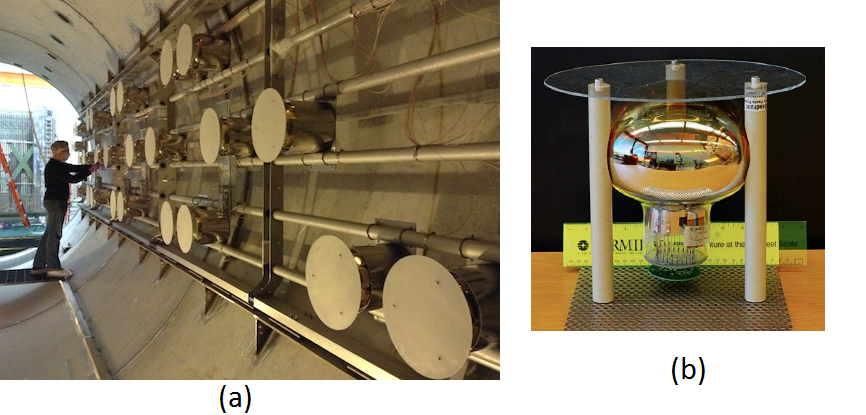
\includegraphics[width=120mm,scale=1.0]{figures/pmmb.png} \caption{(a) Placement of the PMTs in MicroBooNE \cite{SDP}, (b) A PMT. In front of each PMT there is a wave-length-shifter acyclic plate which shifts the scintillation light to blue region since the PMT is not sensitive for VUV light \cite{MR}.} \label{fig:pmmb} \end{figure}  
\\Figure \ref{fig:events} shows summary of expected event rate, in 60 tons active volume of MicroBooNE, these rates are predicted by NUANCE which is a neutrino simulation software.
\begin{figure}[h!] \centering 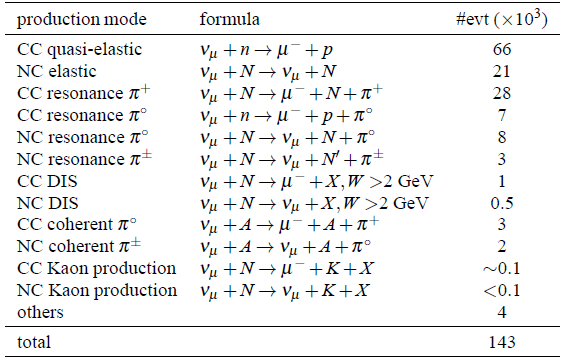
\includegraphics[width=120mm,scale=1.0]{figures/events.png} \caption{Summary of expected event rate 468 m far away from the BNB target, in 60 tons active volume of MicroBooNE, these rates are predicted by NUANCE \cite{MR}.  } \label{fig:events}\end{figure}  
% (IN THE SOURCE IT IS WRITTEN "6E20 POT", WHAT DOES IT MEAN?) ->protons on target
\end{comment}

Drift velocity in the TPC is one of the most important parameters one needs to know to be able to reconstruct the ionization track. It depends on the electric field applied to the medium and the temperature of the LAr \cite{NKR}. 
\begin{comment}
JAMES didnt want this.
Figure \ref{fig:dv} one can see dependence of drift velocity on the electric field.
\begin{figure}[h!] \centering 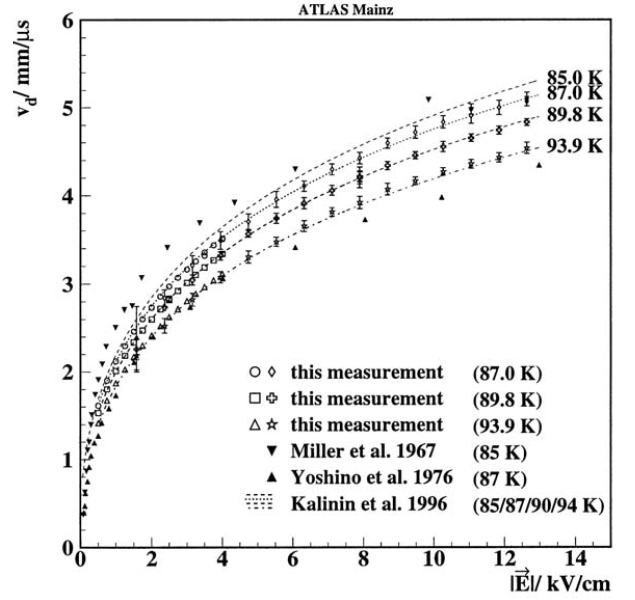
\includegraphics[width=120mm,scale=1.0]{figures/dv.png} \caption{Drift velocity in the TPC is one of the most important parameters we need to know to be able to reconstruct the ionization track. In this figure results of different experiments are showed. \cite{NKR}}\label{fig:dv} \end{figure}  
\end{comment}
The maximum drift time in MicroBooNE, which means the time needed to pass through 2.5~m, is 2.3~ms. The readout time is 4.8 ms \cite{1}, it is higher than the maximum drift time in order to be sure that all of the ionization electrons from previous events are collected. 
Disadvantage of longer drift time is to be exposed to more cosmic rays. Moreover, if the time of an event is not known very well, it can be mistaken with the events occurred in the beam time.

%Longer drift distances need purer LAr for a good charge collection. In MicroBooNE life time of a free electron is 15 ms which corresponds to 0.02 ppb (parts per billion) oxygen-equivalent impurity.
%In MicroBooNE for greater than $50~\%$ charge collection one can allow up to 100 ppt (parts per trillion) oxygen-equivalent impurity \cite{MR}.

\subsection{Why does the SBN Project need a CRT?}
At sea level the most abundant energetic charged particles are muons, about 1~muon $\mathrm{cm}^{-2}~\mathrm{min}^{-1}$ \cite{muos}. They are produced about 15 km above the sea level and have 4 GeV average energy when they reach the earth.

MicroBooNE is placed inside a 12 m (length) $\times$ 3.8 m (diameter) cylindric cryostat. In this volume, the number of cosmic muon-induced events is on the order of 10 for every drift. The biggest danger is not the muons inside the active volume, because we can already see them after the charge collection, but instead muons which interact with LAr outside of the active volume. 
Photons which are created in the interaction of the muons with the detector can enter to the active volume and produce signals which can be misidentified as electron neutrino events.
To achieve its physics goals, the SBN project must minimize this cosmic-ray-induced background.
%To operate the experiments at underground in order to have a natural background-shield is an option, as in SNOLAB \cite{snolab} which is a laboratory at 2 km underground. As it is mentioned before, DUNE's far detector will be at 1,475 m underground, at this depth the expected muon rate is one muon per hand-sized area per year \cite{dunm}. To go deep underground is not easy and not the only solution against the background. 
Cosmic ray taggers which use coincidence to identify background can achieve this.

The CRT in the SBN project covers the TPCs and creates a muon telescope in order to determine position of the ionizing charged particle. It allows to mitigate the effect the cosmic background and make measurements in the TPCs more reliable.
In the following chapter the details of the CRT will be discussed.

\begin{comment}
``Dirt event" is described as any backgrounds generated in the interaction of beam neutrinos outside of active volume of the TPC \cite{prop}. Since dirts event can be occurred inside the TPC, CRT cannot avoid these backgrounds. Since photon has a short radiation length in LAr (14 cm), the LAr inside the cryostat outside of the TPC's active volume creates a shield against the photons which may enter to the active volume from outside. Moreover, in order to have a thicker LAr-shield against any background photons, fiducial volume of the TPC is restricted to 30 cm from the up and 25 cm from the side boundaries of the active volume of the TPC.
\end{comment}

%CRT will cover all around the TPCs. CRTs create a muon telescope which theoretically has standard deviation (coordinate resolution) of $L/ \sqrt{12}$ where L is length of bar in the CRT.

                                                         %ADD HERE LATER
%\begin{figure}[h!] \centering 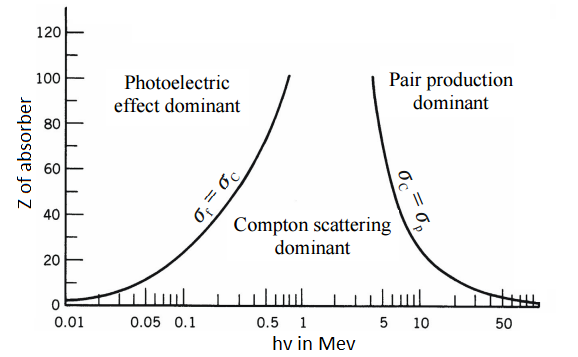
\includegraphics[width=100mm,scale=1.0]{figures/photon.png} \caption{Dominance regions of interactions of gamma-ray respect to its energy. Adopted from [F]} \end{figure}  
%For energies above 100 MeV the major interaction type of the photon is pair creation, for electron after 100 MeV bremsstrahlung plays the main role about losing the energy.
%\begin{figure}[h!] \centering 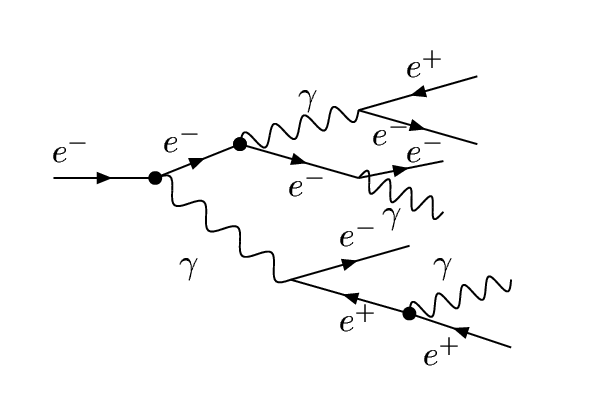
\includegraphics[width=100mm,scale=1.0]{figures/shower.png} \caption{An electromagnetic shower induced by an electron. [G]} \end{figure}  
%A muon can create a shower after about 30 GeV, if we think that the mean energy of the muons at sea level is about 4 GeV, we can understand why electromagnetic showers are every time related with electrons or photons.

%%%%%%%%%%%%%%%%%%%%%%%%%%%%%%%%%%%%%%%%%%%%%%%%%%%%%
\clearpage
\section{Cosmic Ray Tagger}
\label{chap:crt}
The cosmic ray tagger is made of planes, e.g. MicroBooNE has 4 planes, % perpendicular to the neutrino beam direction which consist of modules that will be described in the following.
which consist of modules. % that will be described in the following.
In this section, the fundamental components of our CRT system and how to build a CRT module will be presented.
From December 2015 to October 2016 I built 70 modules in the laboratory in Bern.

Each CRT module includes 16 scintillator strips, see Figure \ref{fig:tapes}, and is able to provide a 1-dimensional spatial coordinate for an event generated by a through passing particle.% and 2 timestamps for each event. 
\begin{figure}[h!] \centering 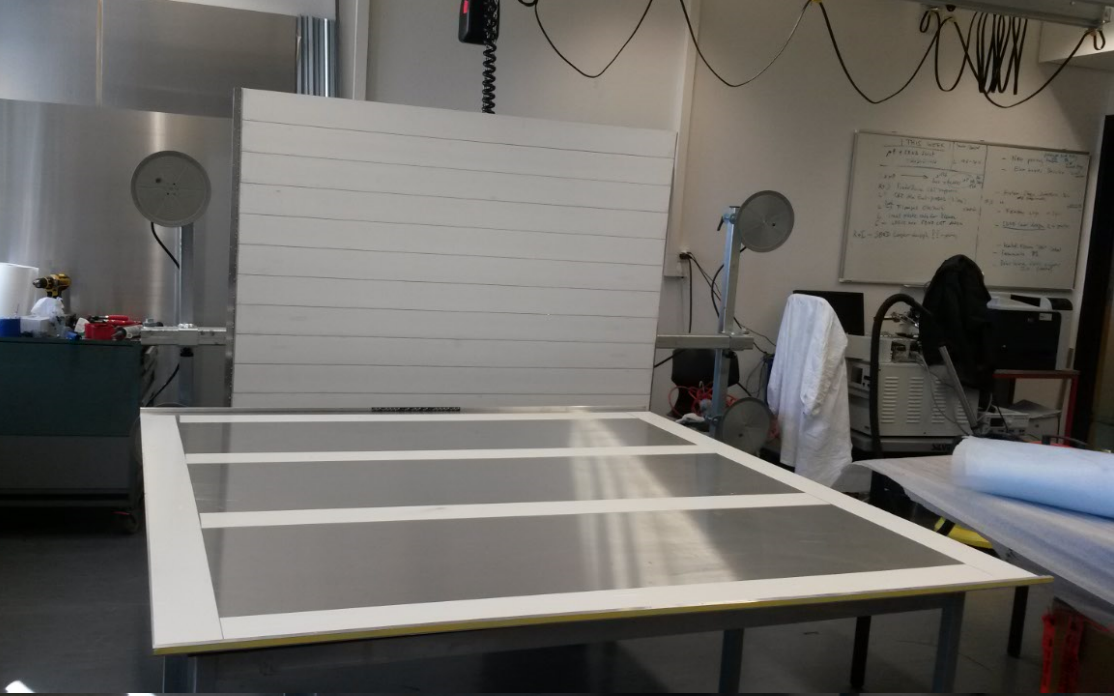
\includegraphics[width=120mm,scale=2.0]{figures/tapespaint.png} \caption{A $1.8\times 1.8$~$\mathrm{m^{2}}$ CRT module. On the background one can see the scintillator bars which are sticked on an aluminium plane via double sided sticky tapes. And on the foreground one can see how the sticky tapes are positioned on an aluminium plane. The length of the CRT modules varies from 3.5 m to 4.5 m.}  \label{fig:tapes}\end{figure}
Therefore to determine the 2-dimensional coordinates, one needs 2 modules. 
%In Figure \ref{fig:crt}, you can see how the modules form a plane. \begin{figure}[h!] \centering 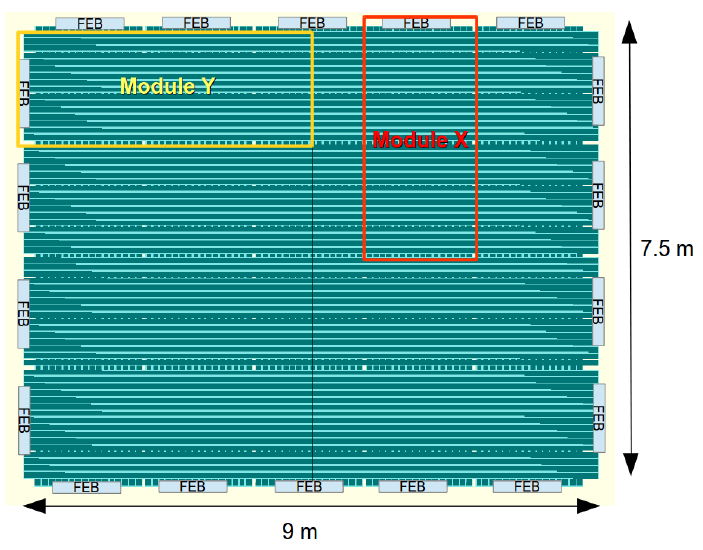
\includegraphics[width=120mm,scale=1.0]{figures/crt.png} \caption{A CRT plane which will be used in SBND. It consists of 18 CRT modules, 10 modules to determine the x coordinate which are aligned vertically and 8 modules for the y coordinate which are aligned horizontally. If we want to determine the 2D coordinates of an event, we need signals from one x module and one y module.  \cite{E}}\label{fig:crt} \end{figure}  
\\The main components of a module are scintillator bars, photo-sensors and wave length shifting fibers which deliver the scintillation light created in the scintillation bar to the photo-sensors. In the following section these three components are presented.

\subsection{Scintillator, Fiber and Multi-pixel Photon Counters}
\label{chap:scifib}

The scintillator material used in the CRT modules is a doped polystyrene, USMS-03, and its ingredients are 98.46 $\%$ Styrolution PS GPPS, 1.5  $\%$ 1,4-Diphenylbenzene (PTP) and 0.04~$\%$ 1,4-Bis (5-phenyl-2-oxazolyl) benzene (POPOP) \cite{C}. USMS-03 has its maximum emission at 430~nm and its effective attenuation length is larger than 8 cm %(BU BULK NE YAW ??) 
\cite{E}.
The surface of the scintillators has been chemically modified to increase the internal reflectivity. Each scintillator strip has grooves on its lateral sides, see Figure \ref{fig:drilled}, these grooves are nests for the fibers which guide the light to the MPPCs.
\begin{figure}[h!] \centering 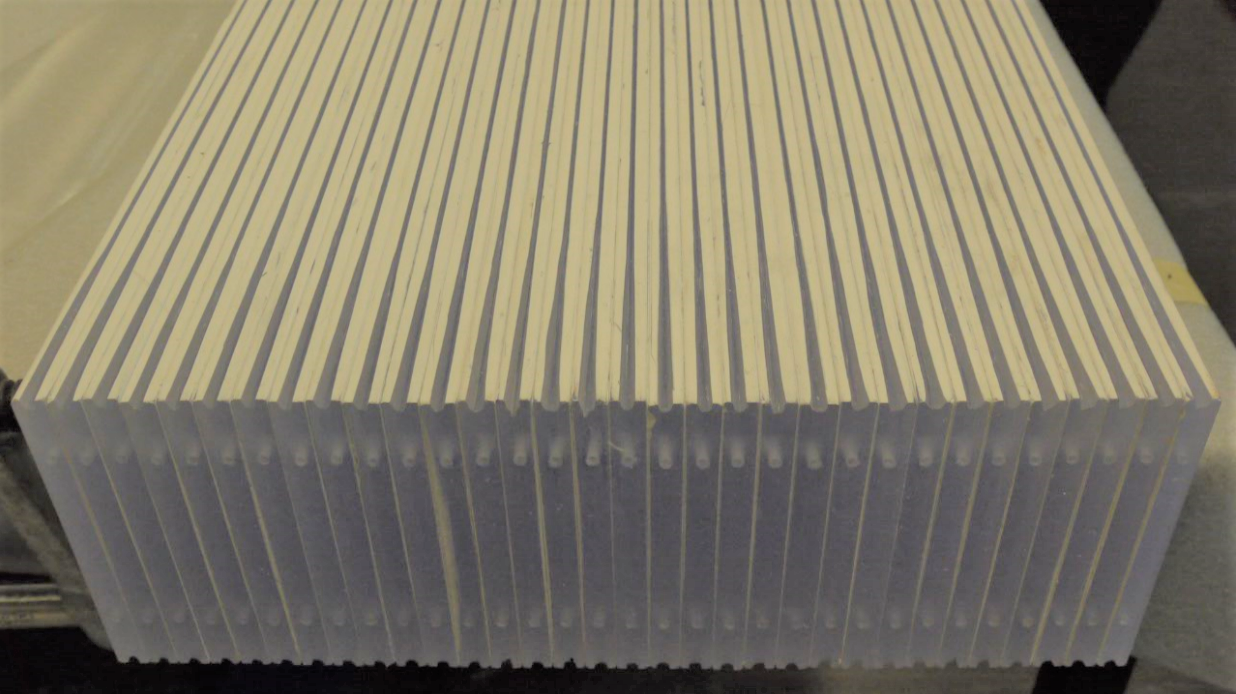
\includegraphics[width=120mm,scale=2.0]{figures/drilledpaint.png} \caption{In the figure one can see the drilled scintillator with their grooves. The grooves will host the fibers. The beginning of them are expanded in order to avoid bending of the fibers in contact with the MPPCs.}  \label{fig:drilled}\end{figure}

Each scintillator strip has 2 fibers that collect the scintillation light.
Our fiber is a Kuraray Y-11 (200)M 1~mm fiber which has attenuation length $ >$3.5~m~\cite{D}. This is a multi-cladded blue to green shifting fiber of grade 11 with a dye concentration of 200 ppm and a diameter of 1 mm.
Its absorption peak is at 430 nm and the emission peak is at 476 nm. 

The photo-sensors used in the CRT system are multi-pixel photon counters (MPPCs) produced by Hamamatsu  (type no S128-050P), see Figure \ref{fig:mppc}. 
\begin{figure}[h!] \centering 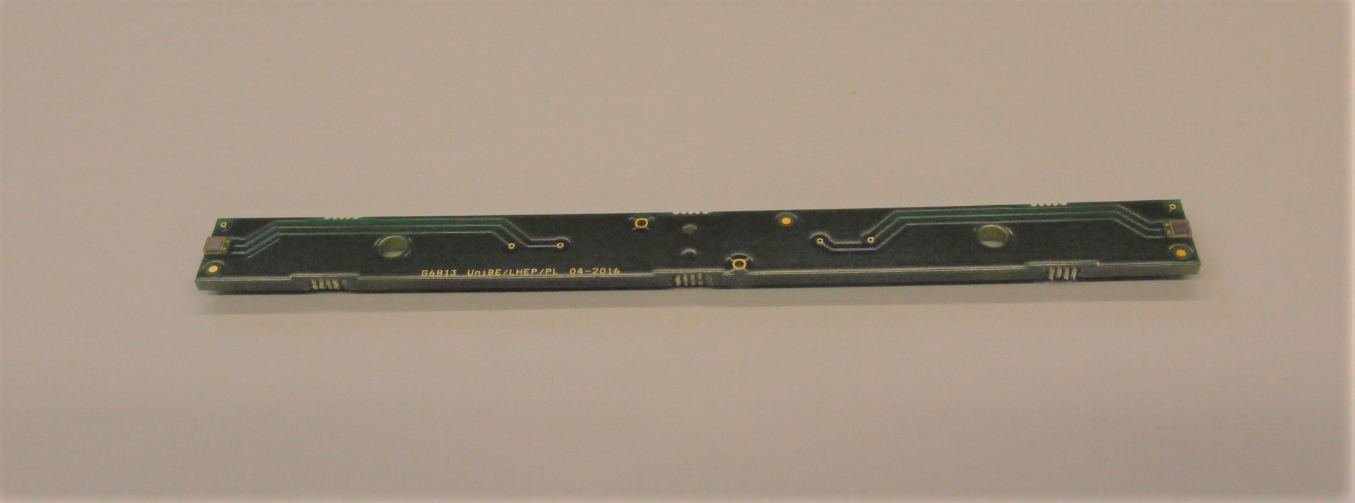
\includegraphics[width=120mm,scale=1.0]{figures/mppcpaint.png} \caption{2 Hamamatsu S12825-050P MPPCs ready for mounting} \label{fig:mppc}\end{figure}  
Some properties of the MPPCs used in the modules can be seen in Table \ref{tab:pprr}.
\\If one considers that the scintillator has an emission peak at 430 nm, the fiber has an absorption peak at 430 nm and an emission peak at 476 nm and the MPPC has an absorption peak at 450 nm, this is a good combination.
\begin{table}
     \centering
    \caption{Some Properties of the MPPCs used in the modules \cite{hama}. }
     \begin{tabular}{| l | l | l  | l | l |}
        \hline \hline 
        Effective photosensitive area & \(1.3\ \times \ 1.3 \ mm^{2} \)  \\     \hline 
        Pixel pitch & \( 50 \ \mu m \) \\      \hline 
        Window material& \( Epoxy\ resin \)  \\     \hline 
        Window reflective index & \( 1.55 \) \\      \hline
        Peak sensitivity wavelength & \( 450 \ nm ^{*}  \)  \\     \hline 
        Photon detection efficiency at 450 nm & \( 35 \% \) \\      \hline
 \end{tabular}
\label{tab:pprr}

\vspace{1ex}
\raggedright{*Under $T_{ambient}$=25$C^{\circ}$ and $V_{over}$=2.6 V.}
\centering
\end{table}

The components of a CRT module which are presented above reside in an aluminium shield. In the following properties of this shield is discussed.

\subsection{Aluminum Shield}
The main aim of the aluminum shield is to serve as a mechanic protection case. Besides, it protects the scintillator bars and the MPPCs against low energetic electron and photons.
In order to reveal functionality of radiation shielding with aluminum, in the following radiations emitted by $\isotope[40]{K}$ which has a big abundance in our living areas will be used as examples.

The attenuation length of a material is defined as the distance over which incoming gamma ray's intensity drops to $1/e$ of its initial intensity and varies with the energy of the gamma. 
The energy of the gamma emitted by $\isotope[40]{K}$ is about 1.5 MeV. In dry air attenuation length for these gammas is 15.22 m which means that in a small room most probably the gammas emitted from $\isotope[40]{K}$ in the walls will reach our modules. In aluminum, attenuation length of 1.5~MeV gammas is about 7.5~cm. If we consider that the thickness of the aluminum we use is 2 mm, the aluminum shield is not enough thick to avoid the gammas emitted by $\isotope[40]{K}$. But this is not a problem because the background rate is reduced by using basic coincidence between MPPCs.

%Here, one of the most important parameter is radiation length and can be approximated by the following formula 
%\begin{equation}X_{0} = \frac{716.4 \ A}{Z (Z + 1)\ ln \frac{287}{\sqrt{Z}}} \ g \ cm^{-2}, \end{equation} 
%where Z is the atomic number and A is mass number of the medium. By dividing this formula with density of the medium one can get the, on average, the length that a high energetic charged particle has $1/e$ of its initial energy. %and  it is equal to a 7/9 of mean freepath to make a pair production by a high energetic gamma. bu kirmizi yeri bi arastir, sadece wik boyle soyluyor. 

Another important parameter is $- dE/dx$ which describes the energy loss of a particle due to interaction with the matter. Since this loss changes with energy of the incoming electron one needs to use the continuous slowing down approximation (CSDA) range which gives the approximate average propagation distance for a charged particle while it is slowing down. 
Potassium-40 emits also 1.31 MeV electrons. In dry air, their specific CSDA range is about $6.47~\times~10^{-1} \ \mathrm{g/{cm}^{2}}$ \cite{csda} which tells us that these electrons propagate about 0.23~cm in dry air and they would not reach our modules. 
Still let us assume that a 1.31 MeV electron reached the aluminum shield. In aluminum its  CSDA range is $7.24 \times 10^{-1} \ \mathrm{g/{cm}^{2}}$ \cite{csda} which results in a 0.26~cm propagation distance. This means that the thickness of our aluminum shield is not enough to stop it but since the electron does not have enough energy to create an electromagnetic shower inside the scintillator bars, again $\isotope[40]{K}$ does not create a problem for the CRT modules. 
%\\Still a high energetic electron or photon can come and create a shower inside a module, this can create an valid event, even, with a small possibility, this shower can effect 2 different modules which are in coincidence.

Another important component of a CRT module is Frond-End Electronics Board (FEB) which is designed to readout a module. In the next section its properties and working schema is presented.

\subsection{Frond-End Electronics Board}
The FEB provides individually adjustable-voltages to the MPPCs, amplifies, shapes and digitizes the signals that come from MPPCs as well as takes coincidence between the signals. 
\\In Figure \ref{fig:cp} one can see the analog to digital converter spectrum (ADC spectrum) of a FEB. The ADC threshold is 250 in order to cut the first peak of the spectrum which represents the baseline of the electronics (pedestal). The pedestals of the related channels are in Figure \ref{fig:pd}. One can see how the baseline of the electronics fluctuates.
\begin{figure}[h!] \centering 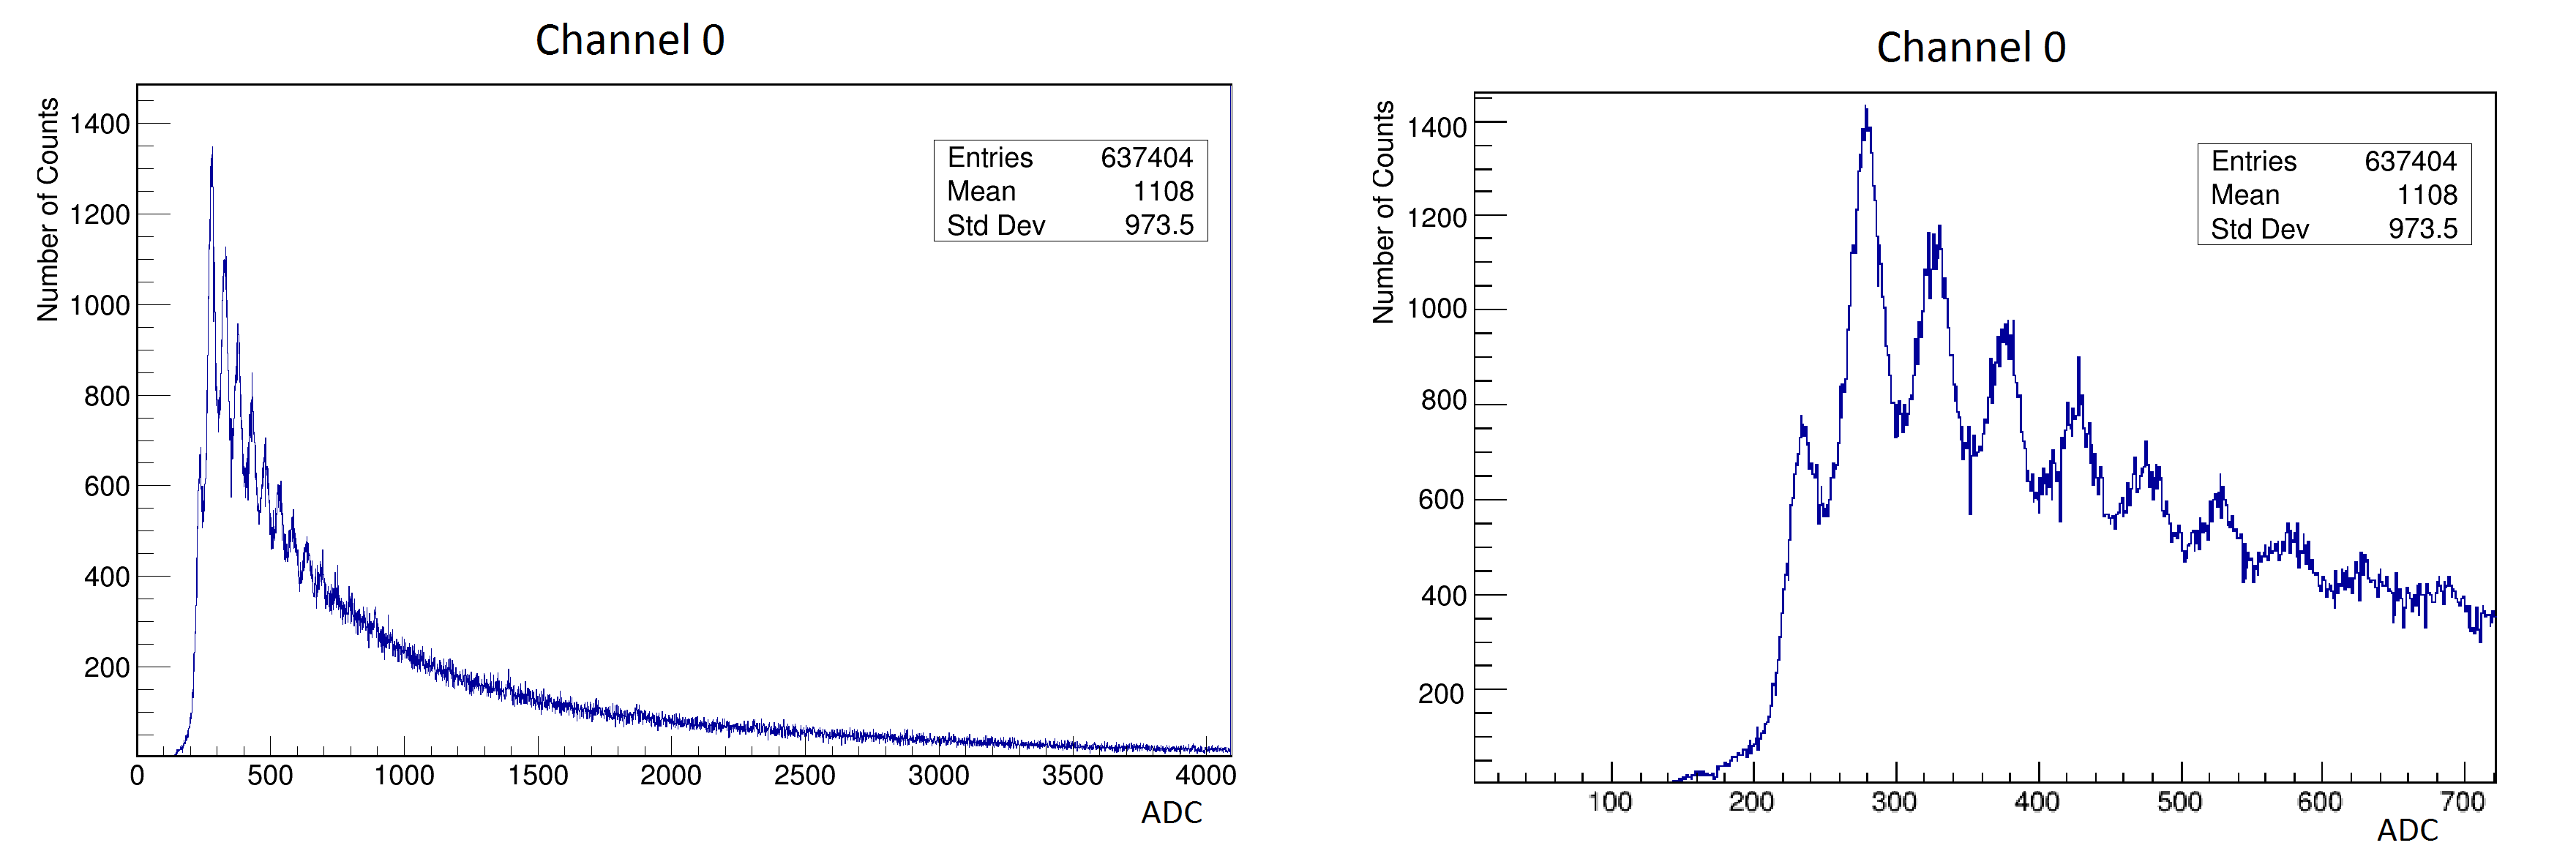
\includegraphics[width=130mm,scale=1.0]{figures/cp.png} \caption{Left, ADC spectrum of a 1.7 $\times$ 5 module's zeroth channel. Right, zoomed on the beginning of the spectrum in order to show the photon peaks better. }\label{fig:cp} \end{figure}
\begin{figure}[h!] \centering 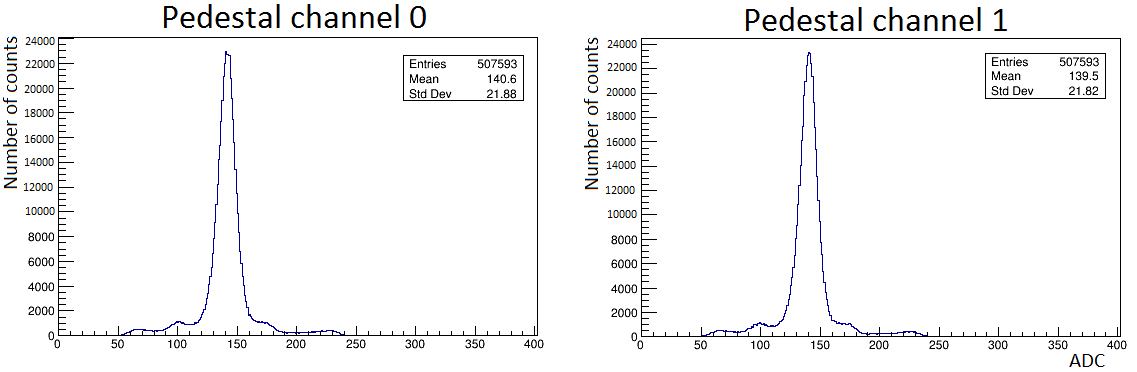
\includegraphics[width=130mm,scale=1.0]{figures/pd.png} \caption{Left, pedestal spectrum of the related module's zeroth channel, and at the right the pedestal spectrum of the first channel. In the figure one can see how the baseline of the electronics fluctuate. To get pedestal of an MPPC one should take measurements without enabling it. Since the pedestal will come out as an output of the other MPPCs's measurements, it would boot the process to enable all of the other MPPCs of the CRT module.} \label{fig:pd}\end{figure}

In order to keep track of all the actual information on the FEBs, a data basis has been created. For details of this data basis see Appendix \ref{App:AppendixA}.

One can summarize working process of the FEB as below.

\subsubsection{Bias Generation}
FEB supplies bias voltages to the MPPCs by a switched-mode power supply that operates at a frequency of 100 MHz. A switched-mode power supply is a device that performs electric power conversion by using a switching regulator. This technology has a very high power efficiency and thus low heat dissipation. The bias voltage is adjustable between 50 V and 90~V. 
\\It is possible to fine adjust the bias voltage individually for each MPPC, this is performed by 8-bit DACs inside the CITIROC chip which is a 32-channel front-end ASIC (Application-Specific Integrated Circuit) and designed by OMEGA \cite{omega} to readout analog signals of MPPCs. The DAC adjusts the bias by applying a positive voltage against the bias voltage.

\subsubsection{Analog Signal Readout}
After the FEB receives the signal from the MPPC, the signal is amplified and shaped by a RC-CR slow shaper with a configurable peaking time of 12.5 to 87.5 ns. Then it is stored inside a hold circuit until it is sent to an analog multiplexers upon request of the CPU, to digitize the desired output signal of the 32 channels. This primary process occurs inside the CITIROC. If the CPU of the FEB receives a trigger signal, it starts the readout cycle and sends out the amplitude information of the channels encoded in 12 bits.

\subsubsection{Triggering}
The triggering process of the MPPC signals starts in the CITIROC. 
\\The CITIROC firstly amplifies the received 32 charge signals with a configurable gain, then a fast RC-CR shaper shapes the signal with a peaking time of 15 ns and sends it to the discriminator. The discriminator can be enabled or disabled on a per-channel basis. The discrimination threshold is adjustable per channel by means of a 10-bit DAC. The next station of the signal is a SPARTAN-6 FPGA (Field-Programmable Gate Array) which computes the coincidences between each pair of channels of one scintillator strip via AND gates whose outputs are combined using an OR-gate. The diagram of the circuit can be seen in the Figure \ref{fig:trig}. \begin{figure}[h!] \centering 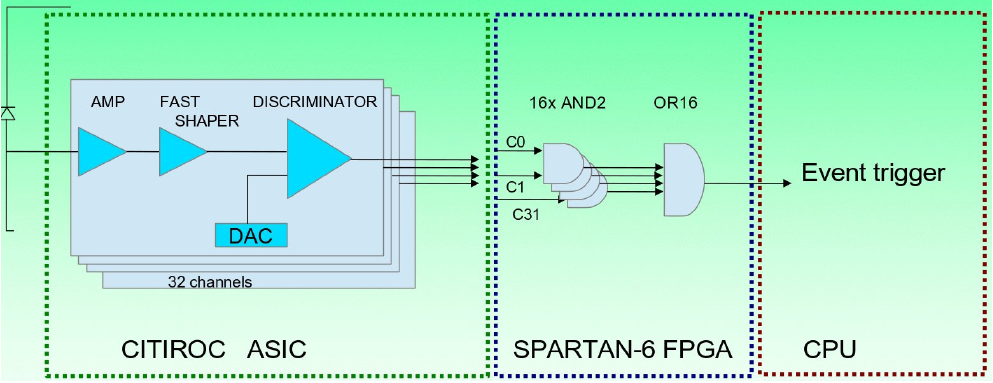
\includegraphics[width=120mm,scale=1.0]{figures/trig.png} \caption{Triggering circuit \cite{E}} \label{fig:trig} \end{figure}
The output of the OR-gate starts the triggering in the CPU as well as a time stamp generator. 

The time stamp generator consists of a clock which runs at a frequency of 250~MHz (4 ns period), and a delay-chain interpolator which incises the accuracy to 1~ns. The time stamp is created by reading out a 1~ns counter which is reset every second by a precise GPS signal. The FEB also allows to give a second time stamp to an event. 

50 ns after triggering, a "Hold" signal, which is logic 1, is triggered and the hold circuit stories the amplitudes of the signals. This "Hold" signal is also routed to "TOUT" which is connected to "TIN" of partner modules to activate their readout window for 150 ns, see Figure \ref{fig:tout}. If during this 150 ns the FEB of one of the partner modules get an internal triggering signal, the event will be accepted as a valid event and the CPU converts the analog signal to digital. After that 150 ns the CPU resets the hold circuit with a logic 0 that lasts for 150 ns. If there is no signal from TIN, the SPARTAN-6 resets the hold circuit with logic 0. 
\begin{figure}[h!] \centering 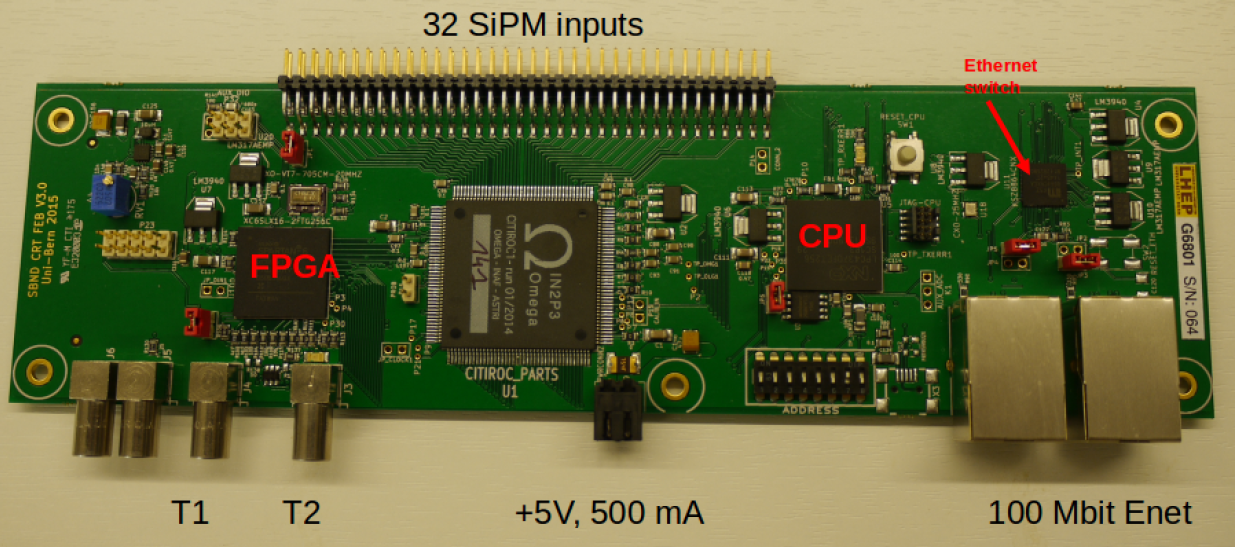
\includegraphics[width=120mm,scale=1.0]{figures/tout.png} \caption{ A FEB without its protective cover \cite{E}} \label{fig:tout} \end{figure}

This wait and reset process allows to take coincidence between 2 modules. With other words, the first module sends a signal through TOUT and if it gets a signal through TIN during its 150 ns Hold signal, this is a valid event. %Length of time of logic 0 and 1 is chosen in such a way that this time is enough for the signals to travel the largest CRT. bu konuyu tam anlamadim, hangi signal?
Since the peaking time is 15 ns, the coincidence window varies from 0 to 30 ns, depending on the amplitude of the signal with respect to the discriminator threshold. % disc. treshold ne bizde?

After converting the analog signals to digital, the CPU combines them with their time stamps and stores them in an internal ring buffer which has a capacity of 1024 events capacity. The ring buffer is readout by the back-end via the Ethernet ports.

\subsection{Tests with Prototype Module}
\label{chap:proto}
In this section, some of the tests which were done with the first produced module, a 1.7x5 m prototype, will be presented. Between the prototype and the modules we produced later on there are very small changes which do not create any effects on the measurements.

\subsubsection{Muon Detection Efficiency}
A muon detection efficiency experiment of the prototype module was performed with help of a muon telescope which has the same experiment setup described in Chapter \ref{chap:measurements}. Basically this setup compares the number of counts in the telescope and the number of counts in the module which works in coincidence with the telescope. Let N1 be the number of the counts in the telescope and N2 the number of counts in the module,  then the detection efficiency is N2/N1.
In Figure \ref{fig:eff} one can see the experiment results \begin{figure}[h!] \centering 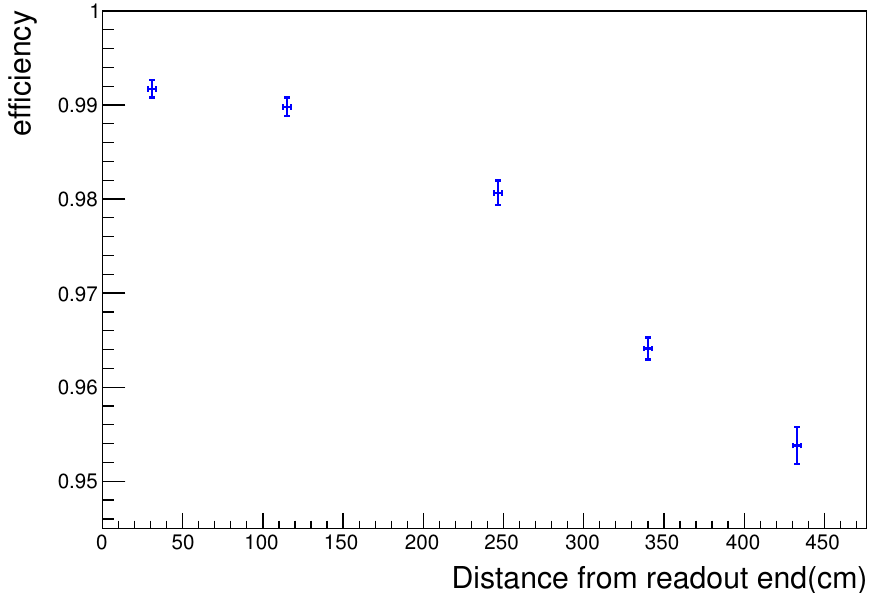
\includegraphics[width=120mm,scale=1.0]{figures/eff.png} \caption{Muon detection efficiency measurements of the prototype module.Let N1 be the number of the counts in the telescope and N2 the number of counts in the module,  then the detection efficiency is N2/N1. \cite{E}} \label{fig:eff}\end{figure} 

\subsubsection{Light Yield}
Light yields of a scintillator bar for cosmic muons at different distances from the readout end were measured. These measurements also were made with the experiment setup described in Chapter \ref{chap:measurements}. 
The CRT module was placed between PMTs of a muon telescope and at each position the number of photoelectrons created by incoming radiation was observed. In Figure \ref{lyo}, one can see the average number of photoelectrons with respect to the measurement distance. The y axis represents the light yield in terms of photoelectrons while the distance is on the x axis. 
%Using the exponential attenuation law, $I = I_{0} \ e^{- x/\lambda}$, one can calculate the attenuation length $\lambda$ of the scintillating bar. For this measurements, $\lambda = ??$ \cite{E}.
\begin{figure}[h!] \centering 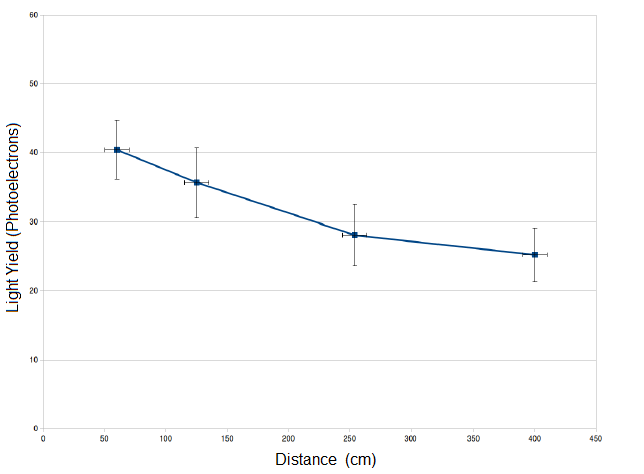
\includegraphics[width=135mm,scale=1.0]{figures/lyo.png} \caption{Light yield of the prototype module's 16 scintillator bars. The light yield is represented in terms of photoelectrons, on the y axis, and the distance is in cm, on the x axis. \cite{E}}  \label{lyo} \end{figure}

\subsubsection{Time Resolution}
A time resolution experiment was made with the help of a 400 nm, 60 ps laser. The laser was placed in between the two fibers of the bar to create scintillation inside the bar. 
\begin{figure}[h] \centering 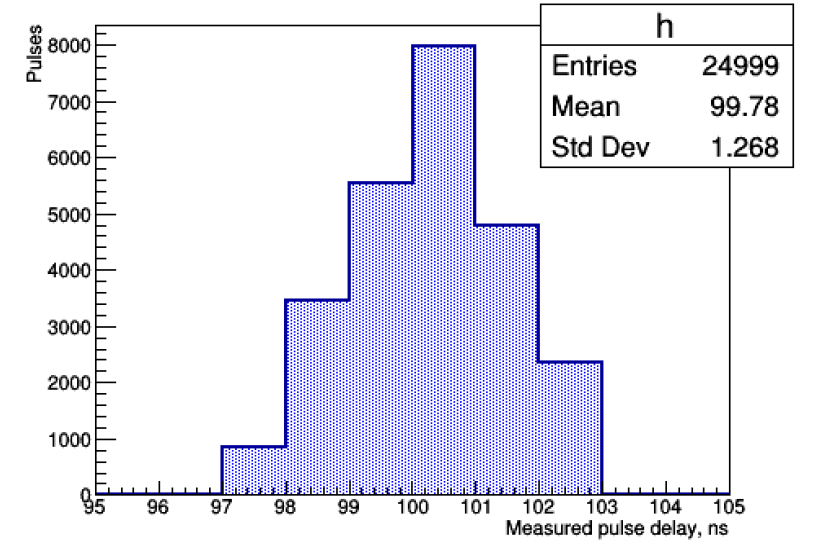
\includegraphics[width=110mm,scale=1.0]{figures/trs0.png} \caption{Time resolution of the prototype module \cite{E}.} \label{fig:trs0}\end{figure}
A T0 signal, which is also sent to the FEB, triggers the laser. The event time is the time difference between the T0 signal and the trigger signal created by the scintillation in the FEB. The results, which can be seen in Figure \ref{fig:trs0}, show that the time resolution is 1.3 ns.

%burda laseri fiberlerin tam ortasina mi koymuslar?

\subsection{Production Procedure of a CRT Module}
The production of a module includes a lot of steps which need to be done very carefully. In Appendix \ref{App:AppendixC} the production steps are described with details. A quick summary can be given as the following;
\begin{itemize}
\item Preparation of optical glue,
\item Cutting of fibers,
\item Depositing mirror on far end of fibers,
\item Cleaning of MPPCs,
\item Preparation of scintillator bars,
\item Preparation of aluminum case and assembling of the scintillator bars.
\end{itemize}

In the preparation of the optical glue, the stiffness of the glues is very important. The glue should not dry for too long or be heated too much because the polymerization speed depends on the temperature of the glue.

The fibers are glued into the grooves with the silicon glue mix and their upper parts are covered with a reflective Mylar in order to protect the fiber and reduce scintillation light loss. Both ends of a fiber are diamond-cut and the far end is coated with aluminum in order to reflect the light towards the MPPC. 
The fibers are quite sensitive to bending. If they are bent too much, they may break or fracture lines can be develop.

On the path of the photons there should be no dirt, the photons could be absorbed or scattered from the dirt. That is why the optical glue, the MPPCs and the fiber nests on the scintillator bars should be very clean.
%%%%%%%%%%%%%%%%%%%%%%%%%%%%%%%%%%%%%%%%%%%%2%%%%%%%%%
\clearpage

\section{Position Determination and Calibration}
\label{chap:pdc}
To determine the position of a charged particle in a module, the scintillation light created by the particle is used. 
In this chapter, I described the light propagation in the scintillator bar and showed how to use this light to determine the position of a charged particle.
%event's signals in the MPPCs, the most important effect that makes this determination complicated is reflection on the borders of the scintillator bars.
%In order to find the best explanation for the practical case, I want to start from the simplest case and then add the effects and practical limitations into it.

\subsection{Light Propagation}
\label{chap:lightpro}
To reach description of light propagation in a scintillator bar, let us start from the simplest movement of a photon; propagation in free space.

As a fist approximation, scintillation light created by a charged particle can be accepted as it is emitted from a point-like source. Since thickness of the scintillator bars is much smaller than width of the bar this approximation is reasonable for the ionizing particles which pass through the thickness of the bar. Following an inverse square law, for a point-like isotropic source the intensity of the light decreases proportional to $1/r^{2}$. If one had a light source between two identical light-intensity-measurement devices, the position of the light source can be calculated by comparing the measured light intensities. More clearly 
\begin{equation} \frac{I_{1}}{I_{2}} = \frac{r_{2}^{2}}{r_{1}^{2}}, \label{eq:1bu}\end{equation}
where $I_{1}$ and $I_{2}$ are the light intensities at the distances $r_{1}$ and $r_{2}$.

Another important effect in the scintillator bar is the attenuation due to absorption. After a propagation in an absorber medium by the distances $r$, the initial light intensity $I_{0}$ will be 
\begin{equation}I = I_{0} \ e^{-r/\lambda} \end{equation} 
where $\lambda$ is the attenuation length,
and the ratio of the intensities at the distances $r_{1}$ and $r_{2}$ is given by
\begin{equation} \frac{I_{1}}{I_{2}} = e^{-(r_{1}-r_{2})/\lambda} .\label{eq:bul}\end{equation}
\\Considering both effects by combing Equation \ref{eq:1bu} with Equation \ref{eq:bul}
%,basically the inverse square law says that in Equation \ref{eq:bul} $ \frac{I_{0}}{I_{0}}= \frac{r_{2}^{2}}{r_{1}^{2}} $, 
one gets
\begin{equation} \frac{I_{1}}{I_{2}} =   \frac{r_{2}^{2}}{r_{1}^{2}} \ e^{-(r_{1}-r_{2})/\lambda} .\label{eq:4}\end{equation}
In Figure \ref{fig:gull} one can see the effects of the absorption, the inverse square law and their combination with increasing the distance. 
\begin{figure}[h!] 
	\hspace*{0cm} 
	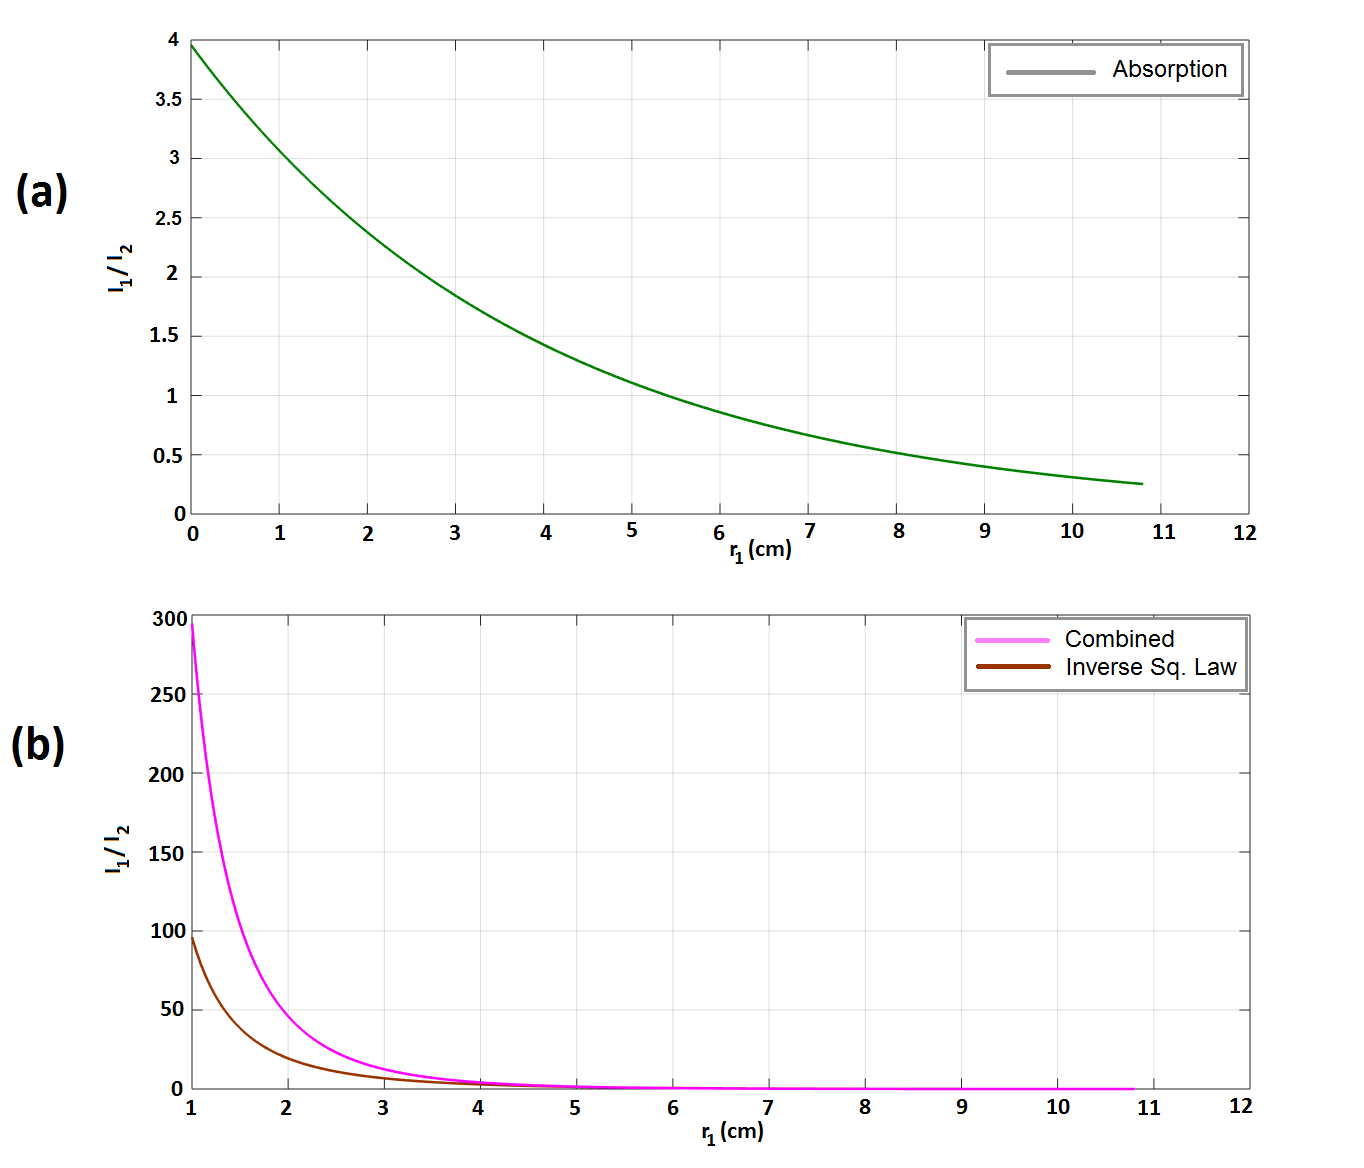
\includegraphics[width=120mm,scale=2.0]{figures/1t.png} 
	\caption{%
	Decrease in $I_{1} / I_{2}$ ratio due to propagation and absorption. $I_{1}$ and  $I_{2}$ are the light intensities at distances  $r_{1}$ and  $r_{2}$. Here $r_{1}$ and $r_{2}$ are the distances measured from opposite sides of the scintillator bar to where the light producing event occurred. $r_{1}+ r_{2}= \ L = 10.8~\mathrm{cm}$ where $L$ is the width of the scintillator bar. This plot is drawn for the attenuation length of $\lambda=7.9~\mathrm{cm}$.  (a) Attenuation of the light due to absorption. (b) The brown line shows effect of the inverse square law and the pink line show the effect of the inverse square law combined with absorption. %The graph starts from  $r_{1}= 1 $ $cm$ because inverse square law gives infinity at $r_{1}= 0 $.
	}
	\label{fig:gull}
\end{figure}
\\Equation \ref{eq:4}, with an approximation, describes the propagation of the light in an absorber medium with infinite volume. But due to reflections it is not sufficient to describe the propagation in the scintillator bars.
In Figure \ref{fig:gull1} one can see the attenuation of the scintillation light inside a scintillator bar with increasing the distance.
This figure is drawn by taking measurement via a muon telescope, for the details of the measurements see Chapter \ref{chap:measurements}, where the scintillation light intensity is obtained in terms of ADC value. In the figure the light intensity is presented in terms of photoelectrons. The relation between ADC value and nubern of photoelectrons ($N_{pe}$) is given by
\begin{equation} N_{pe} = \frac{ADC-P}{G} \label{eq:i1i2},\end{equation} where $P$ is pedestal and $G$ is gain of the MPPC. 
%Without the reflection, inverse square law would be dominant and a big percentage of the scintillating light could not be detected by the MPPCs.
%As it can be seen in the figure, the reflection gives feedback of the propagation. 
%Since reflective index of the scintillating bar is ??? and coating ???, critical angle for total internal reflection is ???. 
%To consider the total internal reflection means to restrict the infinite isotropic, absorbing medium, and to consider reflection from the white surface means to cover around that finite medium with a reflector that this is what we have in the laboratory.
%In Figure \ref{fig:gull1} one can see a measurement of the intensity of light propagating inside a scintillator bar in terms of photoelectrons. In the measurements, the relation between ADC value and photoelectrons (p.e.) is given by \begin{equation} p.e. = \frac{ADC-P}{G} \label{eq:i1i2},\end{equation} where $P$ is pedestal and $G$ is gain of the MPPC.
%One of the reasons create this is high attenuation of the reflected photons, since they travel longer distance they are attenuated more.
\begin{figure}[h!] \hspace*{0cm} 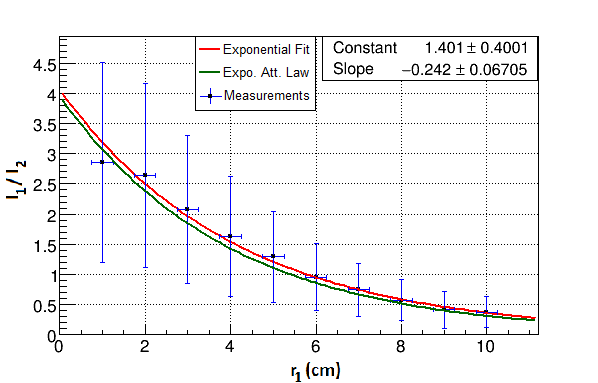
\includegraphics[width=130mm,scale=2.0]{figures/effofre.png} \caption{Measurements of $I_{1} / I_{2}$ ratio together with the expectation of the exponential attenuation law.  
The positions of the amplitudes $I_{i}$, $i=1,2$, are  $r_{i}$ which represent the vertical distances of the fibers to the position of the photon-producing event. The width of the scintillator bar is $ r_{1} + r_{2}=L=10.8$~cm. Red line is exponential fit to the measurements, its fit parameters can be seen in the figure, and the green line shows the expectation of the exponential attenuation law with $\lambda=7.9$~cm.
For this measurement the prototype module was used. } \label{fig:gull1} \end{figure}
\\Without reflection, attenuation would be governed by the inverse square law and a big percentage of the scintillating light could not be detected by the MPPCs. Therefore, the scintillator bar is covered with a reflective coating and thus, attenuation is governed by the exponential absorption law. 

%reflection created a feedback mechanism . and for example, when the incoming radiation pass through the middle of the bar what we expect to see is  $I_{2}/I_{1}=1$, because of the reflection it is possible get this ratio at every positions on the bar. That is why one can say that there is a specific light collection efficiency for of each specific trajectories in the bar.     MAYBE YOU CAN ADD HERE LATER

\subsection{The Coordinate Transfer Function and Its Calibration}
\label{chap:mu}

As shown above, the attenuation of the light inside the scintillator bar is governed by the exponential absorption law.
Therefore the position calculation can be done using Equation \ref{eq:bul} which gives
\begin{equation} \label{eq:pos} r_{i}=\frac{1}{2} \Big(L - \lambda~ln(\frac{I_{i}}{I_{j}})\Big), \end{equation}
where $I_{i}$, $I_{j}$ with $i, j=1,2$, $i\neq j$, are the light intensities at the distance $r_{i}$, $r_{j}$, the width of the bar is $L=r_{i}+r_{j}$, and the attenuation length is $\lambda$. 

In order to calculate the attenuation length of photons across the scintillator bar, an exponential fit to the signals is used. In Figure \ref{fig:mamafi} one can see the attenuation of the light amplitude with increasing the distance where the light amplitude is given in number of photoelectrons. %$1/ \abs{slope}$ of this fit gives us the attenuation length. 
The graph is plotted for a prototype module at 0.5 m from the readout end.
\begin{figure}[h!] \hspace*{-0.7cm}  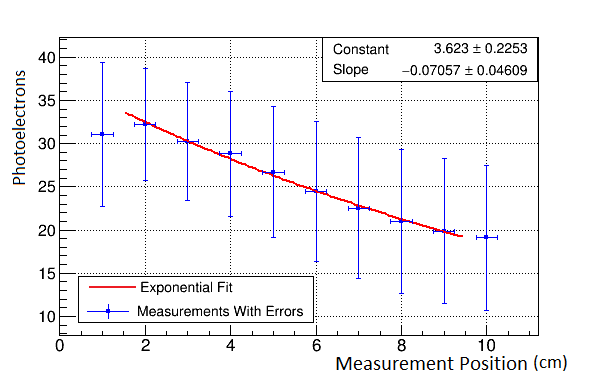
\includegraphics[width=130mm,scale=1.0]{figures/un.png} \caption{Attenuation of the light due to absorption. The fitting formula is $\mathrm{f(x) = exp(Constant + Slope\times x)}$. $\mathrm{1/ \abs{Slope}}$ of this fit gives us the attenuation length. In order to avoid the effect of reflection from the corners, the first and last measurements are not included in the fit. This graph is plotted for the prototype module at 0.5~m from the readout end.} \label{fig:mamafi}\end{figure}  
Here the obtained attenuation length is $14 \pm 9$~cm. %If we draw the same graph for the other channel we get $\lambda=16.8 \pm 12$~$cm$.
%\\The attenuation inside the fiber is negligible compared to the attenuation inside the scintillator. 

As described above, simple measurements gave an attenuation length of $14 \pm 9$~cm. Since the error of this coefficient is big, the attenuation length has been improved by using a different method which will be explained in the following.
%Another reason that justifies this optimization is effect of the light reflection at strip surface. As it can be seen in Section \ref{chap:ref}, the reflection from the surface of the scintillator bar plays an important role on the light collection by the fibers.
\\The best-fit attenuation coefficient is obtained via the least squares adjustment method using Equation \ref{eq:pos}. What we are doing here is to reduce the number of the parameters from two to one ( $\mathrm{f(x) = exp(Constant + Slope\times x)}$ has two parameters, but Equation \ref{eq:pos} has only one) and then apply the least squares method to this one parameter which, as can be seen below, gives a better result.
%In order to find the attenuation coefficient which minimizes the sum of the squared differences between real and calculated positions, 
Thus, the best-fit attenuation coefficient is the one which minimizes the sum
\begin{equation} S=\sum_{n=1}^{N} (r_{n}-r_{1})^{2} \end{equation}
where $N$ is total number of the different measurement distances, $r_{n}$ is the vertical distance of the related fiber to the measurement position 
and $r_{1}$ is the reconstructed distance which is given by Equation \ref{eq:pos}, see Figure \ref{fig:sums}.
\begin{figure}[] \hspace*{-0.7cm} 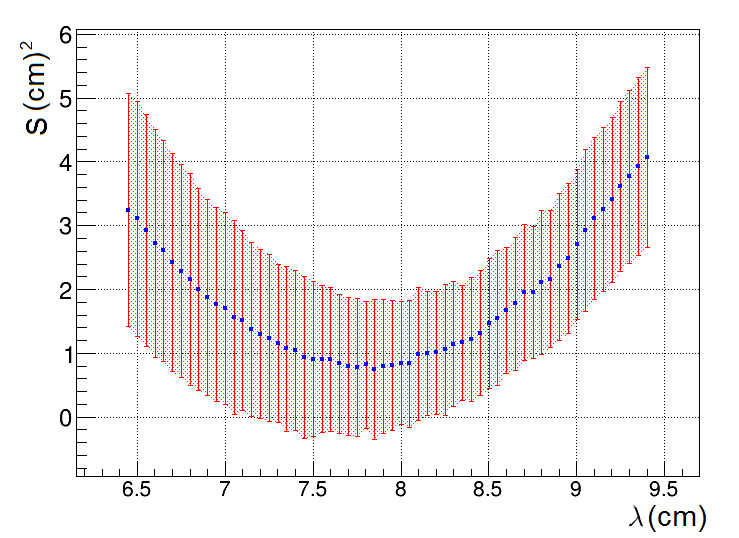
\includegraphics[width=130mm,scale=2.0]{figures/exx.png} \caption {On the vertical axis one can see the
sum of squared differences between measurement and reconstructed distances for 10 different measurement distances and on the horizontal axis different attenuation lengths.} \label{fig:sums} \end{figure}
\\The method described above gives a value of $\lambda=7.9\pm1$~cm for 10.8 cm wide bars and a value of $\lambda=10.5\pm2$~cm for 5.95 cm wide bars. 
Therefore, for the 10.8 cm wide bars the calibrated coordinate transfer function is
\begin{equation} \label{eq:pos11} \mathrm{ r_{1}=\frac{1}{2} \Big(10.8 - 7.9~ln(\frac{I_{1}}{I_{2}})\Big) \ [cm],} \end{equation}
and for the 5.95 cm wide bars
\begin{equation} \label{eq:pos12} \mathrm{ r_{1}=\frac{1}{2} \Big(5.95 - 10.5~ln(\frac{I_{1}}{I_{2}})\Big) \ [cm].} \end{equation}

In the next chapter tests of these functions and their results are presented.

\begin{comment}
But still the exponential attenuation law which governs the absorption does not give the correct position because the most dominant effect on the propagation of the light is the reflection.
%This situation made me feel like I can neglect inverse square law and add the reflection into account as an additional light source, an additional light source toward the fibers and where the light producing event occurred. If there was such a source it would find a place to itself in the exponential attenuation formula, such that basically it modifies the variables around it, that is why i recommend the following formula ?
%\begin{equation}I = I_{0} \ e^{-\mu x + K} ,\end{equation} where K is a variable which has a different value every places in the bar.
%Now the questions is how we will determine value of K if it is a function of the position. I should write it as a function of ratio of light intensities, because this ratio takes a different value at different positions, surely we can expect a symmetry between its values, so
%\begin{equation}K \propto \frac{I_{2}}{I_{1}} ,\end{equation}  we will get $\frac{I_{2}}{I_{1}}$ from measurements, and then take the related values of $K$.
%This model assumes that the light producing particles passes through the scintillator bar vertically, need to be developed via K constant, K or a constant like that can give this information because it is related how much energy released in the bar. (Correct here, and write: graph of K should look like superposition of the curves in graphe1)
%All of the signals from one measurement point should have something common... I should write a formula that gives gives a constant for all of the signals from the same measurement point and whenever i get this constant again, I understand from which position we get the signal, it should consist ratio of the signals and sum of the signals, 
\\One of the problems with the application of the exponential law, which is could be seen in the Figure \ref{fig:gull1}, is standard deviation of the measurements.  To use just ratio of the signals makes the exponential attenuation law very sensitive against the deviations in the signals and this causes the method to give very high standard deviations. 
\\At the left side of the figure the standard deviation is greater than left side because at the left value of $I_{1}$ is bigger than $I_{2}$ and at the right opposite, 
\begin{align*} big \ value/small \ value \to \ big \ standard \ deviation \\
small \ value/big \ value \to \ small \ standard \ deviation.
 \end{align*}
Methods which use every time the same ratio of the signals tend to have greater standard deviations one side than the other side. 
%But this is not a big problem because it can be solved by using ratio of, for example, $I_{1} / I_{2}$ where $I_{2}$ is stronger and ratio of $I_{2} / I_{1}$ where $I_{1}$ is stronger.

From the problems which are mentioned above, we understand that the method will be used for the calibration should not include just ratio of the signals. 
\\For the calibration we recommend center of mass method. Center of mass is defined as the point where the mass distribution is equal in all directions. If one shows the center of mass with C, $i=1,...,n$ points with $m_{i}$ masses
\begin{equation} \label{eq:c} \sum_{i=1}^{n} m_{i} (\vec{r}_{i} - \vec{C}) = 0.\end{equation} 
\\For our case Equation \ref{eq:c} leas to
\begin{equation} C=\frac{I_{1}\ r_{1} + I_{2}\ r_{2}}{I_{1}+I_{2}} ,\end{equation} 
where $I_{i}$, $i=1,2$, is fotoelectron-equivalent of the scintillation light which is released by the charged particle at the position $r_{i}$, $i=1,2$. For us $r_{1}$ is where the scintillator bar starts, 0, and $r_{2}$ is the end of the bar, L.

\subsubsection{Examination of the Calibration Method}
At the point we arrived the calibration formula is
\begin{equation} \label{eq:c1} C=\frac{I_{1}\ L }{I_{1}+I_{2}} ,\end{equation}.
\\In Figure \ref{fig:mamafi} we see how the upper part of the formula behaves against the measurements. Figure \ref{fig:s0pluss1} shows behavior of the denominator.
\begin{figure}[h!] \hspace*{-0.7cm} 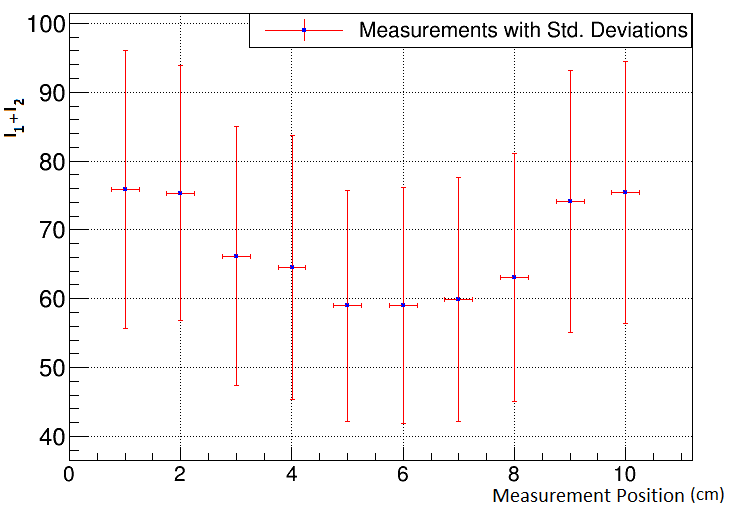
\includegraphics[width=130mm,scale=2.0]{figures/s0pluss1.png} \caption{$I_{1}+I_{2}$ distribution of the measurements. Here we see a symmetric behavior. As long as we get closer to the edges the light collection efficiency becomes better.} \label{fig:s0pluss1} \end{figure}
In the figure we see that as long as we get closer to the edges the light collection efficiency becomes better which is a result of the less absorption, but toward the corners the standard deviation becomes bigger, Figure \ref{fig:s0pluss1s} shows standard deviations in the Figure \ref{fig:s0pluss1} with their standard deviations.
\begin{figure}[h!] \hspace*{-0.7cm} 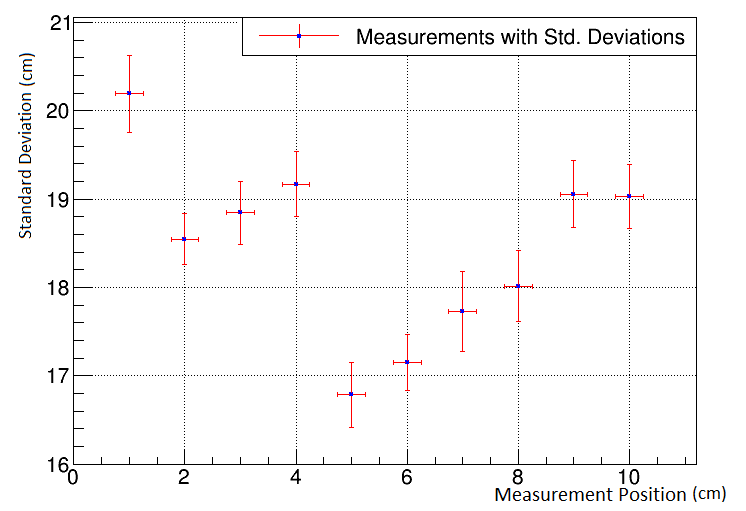
\includegraphics[width=130mm,scale=2.0]{figures/s0pluss1s.png} \caption{Standard deviations of $I_{1}+I_{2}$ measurements.} \label{fig:s0pluss1s} \end{figure}

Now let us see behavior of the equation \ref{eq:c1} for the measurements. Figure \ref{fig:co} shows mass center of the measurements. 
%Here we see an effect, which is we firstly encountered in Figure \ref{fig:gull1}, for the left side of the bar range of the center of mass values $C_{last}-C_{first} \approx 2.4$, for the right side this value is $\approx$...
%Figure \ref{fig:gull1} shows us one more thing for calibration methods; if one wants small standard deviation with the outputs then outputs are confined in a small range which makes the calibration difficult, if one wants larger range such that one can assign the output values to the real values better then the standard deviation is greater. Let us say  ``confinement problem" for it, we will see this effect again.
%  BU KISMI THIN MODUL ILE YAPTIGIN MEASUREMENTLERDEN SONRA BI DAHA DEGERLENDIR. CONFINEMENT PROBLEMI BU MODEL ICIN YOK GALIBA; EN SOL MEASUREMENT AOUTLIER GALIBA; CUNKU BU MODELIN BOLENI SAG VE SOLA GORE SIMETRIK.
The green line represents the middle of the bar.
\begin{figure}[h!] \hspace*{-1 cm} 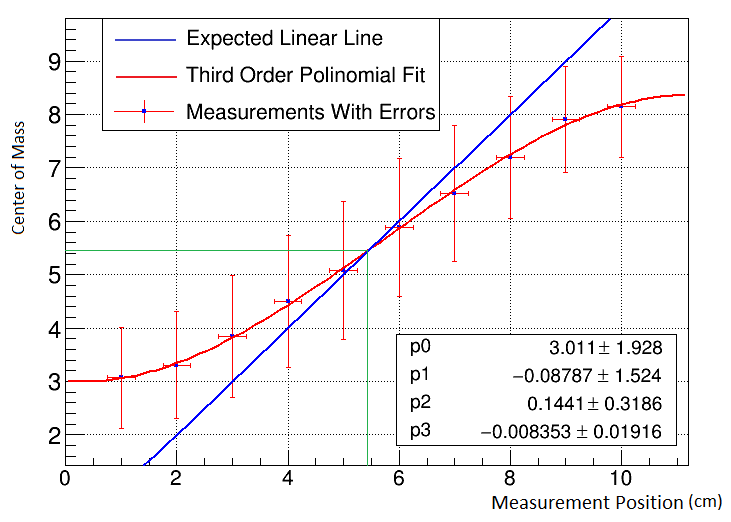
\includegraphics[width=130mm,scale=2.0]{figures/co.png} \caption{Center of mass values of the measurements. The green line shows where the middle of the bar is and which C value is predicted by the third order polynomial fit.} \label{fig:co} \end{figure}
\\Standard deviations on Figure \ref{fig:co} can be seen better in Figure \ref{fig:cos}. Reason of this shape of the figure can be seen in the Figure \ref{fig:s0pluss1s}, small measurements cause bigger deviations. 
We see that at the right side of the bar the standard deviations are slightly bigger than the left side of the bar, this is because at the right side values of the numerator is bigger than at the left side.
\begin{figure}[h!] \hspace*{-1 cm} 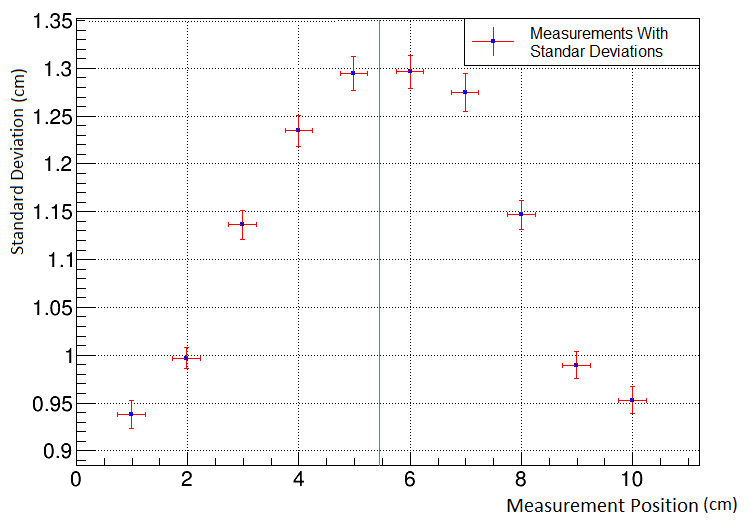
\includegraphics[width=130mm,scale=2.0]{figures/cos.png} \caption{Standard deviation of the measurements with their deviations. The green line shows where the middle of the bar, at the right side of the bar the standard deviations are slightly bigger than the left side of the bar.} \label{fig:cos} \end{figure}

\subsubsection{The Final Calibration Formula}
After the measurements with muon telescope, that detailed measurement procedure can be found in the measurements section, C values of each events at the certain positions are calculated and a graph which shows the difference between mean values of the C values and the positions is drawn. By fitting this graph with third order polynomial fit and the fit parameters are extracted to be used in the following formula in order to reduce the difference between the C values and measurement positions;
\begin{equation} Calibrated= C +\frac{Pol}{F} ,\label{eq:calib}\end{equation} 
where $Calibrated$ is calibrated, position, F is a parameter which is depend on the size of the scintillator bar and $Pol$ is contribution of fit parameters;
\begin{align} Pol=par_{0} + par_{1} \ C +  par_{2} \ C^{2} + par_{3} \ C^{3} \end{align}
here $par_{i}, i=0,1,2,3$ are polynomial fit parameters.
\\Value of F is smaller than 1, it is determined by optimizing measurement results with measurement positions.
%Application of the procedure which is mentioned here can be found in experiment section.

%As I mentioned before, the reflection on the edges has a very big effect on the signals we get from the fibers. This effect becomes more important in smaller scintillator bars. COntinue after your measurements with thin bars





\subsection{Relation Between Propagation Distance of Muon in the Module and Photoelectrons Output}
%(shift 1,2 and 3 cm in 2 different positions... For this I can use different CRTs.)
(If I have time I will do these measurements)

\subsection{Efficiency of the Mirror}
I did not make Damian's corrections for here. You can find it in his e-mail.
There are several variables which effect on the delivered light by the MPPCs from the fibers. The most important ones are; attenuation in the fiber and reflection from the mirror on the far end of the fiber.
In order to observe the effect of the mirror on the collected light, a test has been made. 
\\The bar used in the experiment is 27.5 cm, it is short because we wanted to completely neglect the attenuation in the fibers.
(If I have time I will do these measurements)

\end{comment}

%%%%%%%%%%%%%%%%%%%%%%%%%%%%%%%%%%%%%%%%%%%%%%%%%%%%%
\clearpage
\section{Test of the Calibrated Coordinate Transfer Function}	 
\label{chap:measurements}

To test the coordinate transfer functions I obtained in the last chapter, I used a muon telescope. The sizes of the PMTs are $120\times40\times2.5$~$\mathrm{{mm}^3}$ (upper one) and $90\times30\times2.5$~$\mathrm{{mm}^3}$ (bottom one), see Figure~\ref{fig:2}. \begin{figure}[h!] \centering 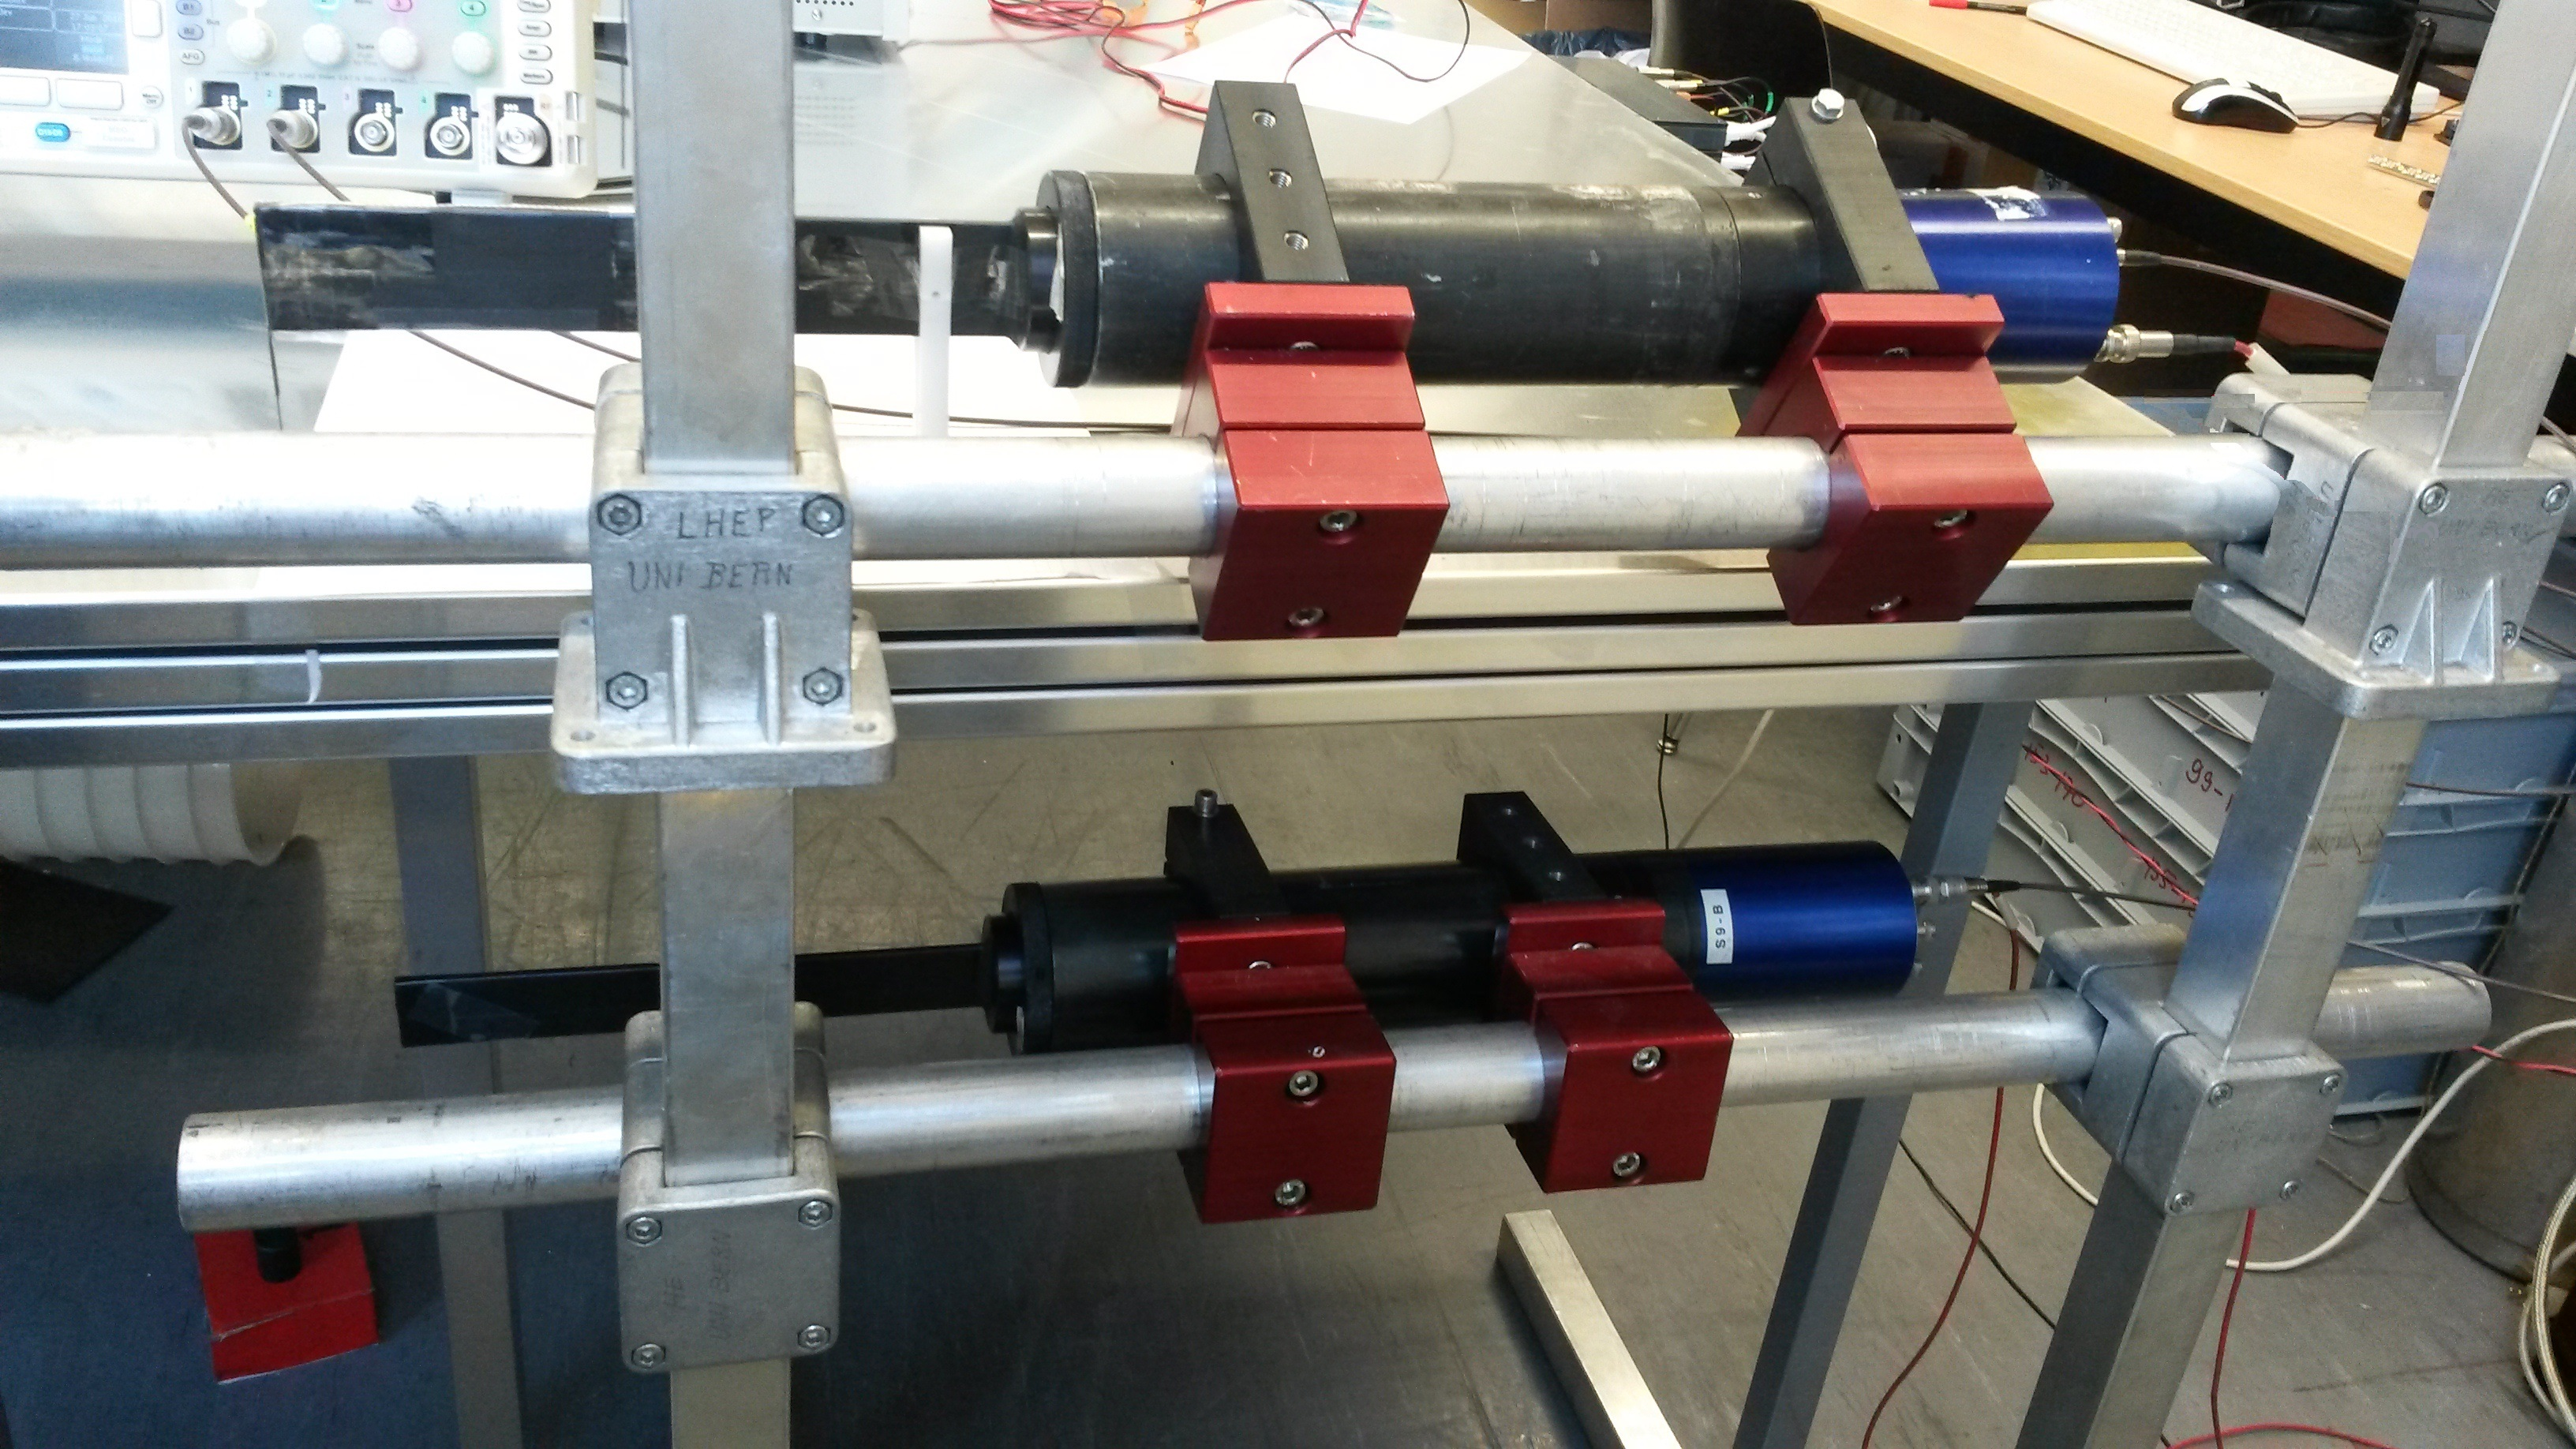
\includegraphics[width=120mm,scale=1.0]{figures/2.jpg} \caption{Photomultipliers together with some of the CRT modules which are used in the measurements.} \label{fig:2} \end{figure}
In the Figure \ref{fig:scheme} one can see the scheme of the telescope connected with FEB.
\begin{figure}[h!] \centering 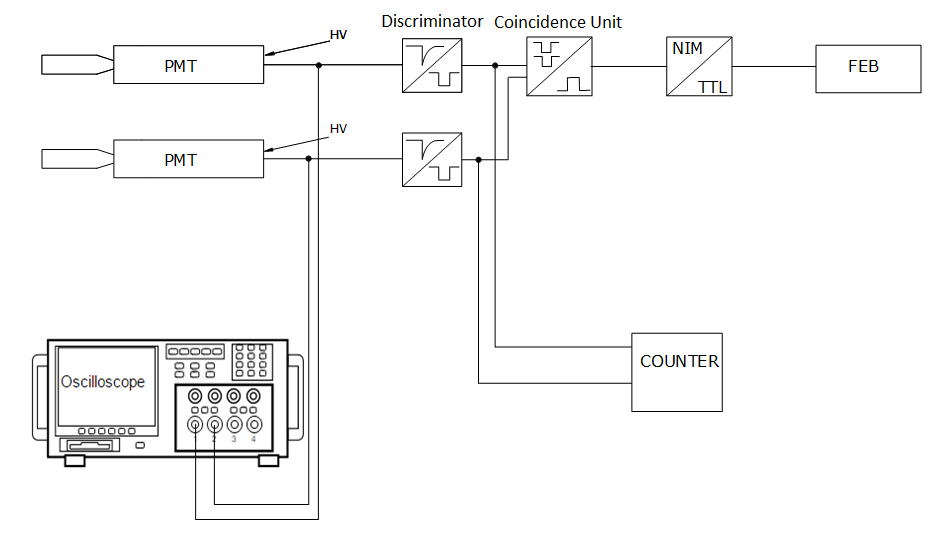
\includegraphics[width=120mm,scale=1.0]{figures/scheme.png} \caption{Scheme of the measurement.} \label{fig:scheme} \end{figure}  

The PMTs are supplied with 2 kV hight voltage. 
First, the output signal levels of PMTs are checked by an oscilloscope to see if they are as we expected. %, when we set the oscilloscope to 200 mV and 40 ms values, we are able to see the proper signals.
As the next step PMTs are connected with discriminator and set the threshold voltage of the discriminator to 30 mV. The threshold is low because the coincidence between the PMTs and the planes will eliminate the accidental coincidence of PMTs. Output  of the discriminator is in NIM format. NIM logic is a current-based logic which gives logic 0 for zero current and logic 1 for -12 to -32 mA under 50 ohm resistance the logic 1 range is –0,6 to –1,6 Volt. %typical dark count of such PMTs is 50 Hz,
\\After this arrangement, the outputs of the discriminator are connected to counter in order to count the events at each PMTs, and then the other outputs of the discriminator are connected to coincidence unit. Input signals of the coincidence unit are terminated by 50 ohm and output of this unit is connected to the counter in order to count the coincidence between the 2 PMTs. Width of the output pulse of coincidence is set to 100 ns, basically this is the width of coincidence window.   
\\The last step is to take coincidence between the PMTs and the CRT module. The output of coincidence unit is a NIM signal. This signal is connected to a NIM to TTL converter. The output of the NIM to TTL converter is terminated the by 50 Ohm resistor and connected to the FEB of the module. 
\\Before sending the output signal of the NIM to TTL converter to the FEB, it is necessary to the check amplitude of the output voltage via an oscilloscope in order to protect the FEB against over voltage. The amplitude of the output signals in the measurements was several volts.

\subsection{Measurements with a 108 mm-wide Bar} \label{chap:108mm}
In the first measurements a $1.7 \times 5$ $\mathrm{m^{2}}$ module which has 108 mm scintillator bar width is used. This module is the prototype which is mentioned in Section~\ref{chap:proto}. Generally the measurements run for one day, number of the counts at each measurement positions can be seen in Figure \ref{fig:pro4}. 
The ratio of the photoelectrons in the MPPCs at each measurement positions can be seen in Figure \ref{fig:gull1}.
%Gain of the Channel 0 is 37.38 and its pedestal is 231.5~ADC, for the Channel 1 gain is 38.53 and pedestal is 230.6~ADC.

As it is mentioned in Section \ref{chap:mu}, for this wide scintillator bars the obtained attenuation length by using our optimization method is $\lambda=7.9\pm1$~$cm$. In Figure \ref{fig:pro1} one can see the calibrated positions. 
Standard deviations of the calibrated positions are presented in Figure \ref{fig:pro2}. 
The scintillator bar is symmetric around its middle point, the model which is used for the position calibration, the exponential absorption law, as well. Because of this one expects to see symmetric errors in Figure \ref{fig:pro2}. The antisymmetric structure in the figure is an experimental mistake.
\begin{figure}[] \hspace*{-0cm} 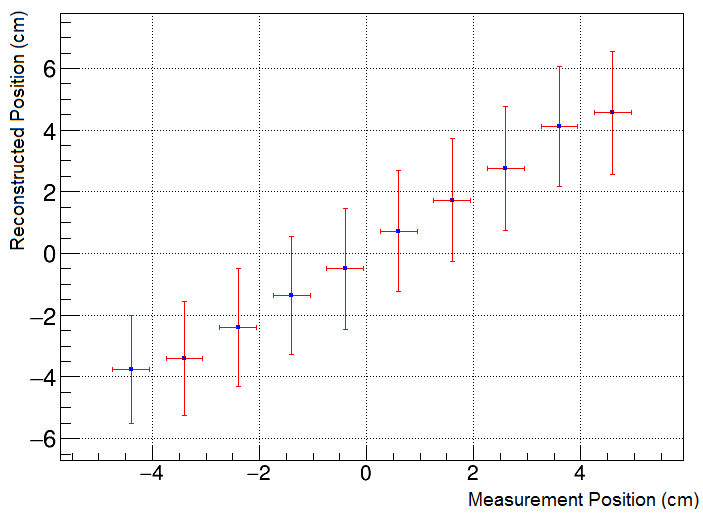
\includegraphics[width=120mm,scale=2.0]{figures/pro1.png} \caption{Calibrated measurements. Here ``0" represents the middle of the bar.}  \label{fig:pro1}\end{figure}
\begin{figure}[] \hspace*{-0cm} 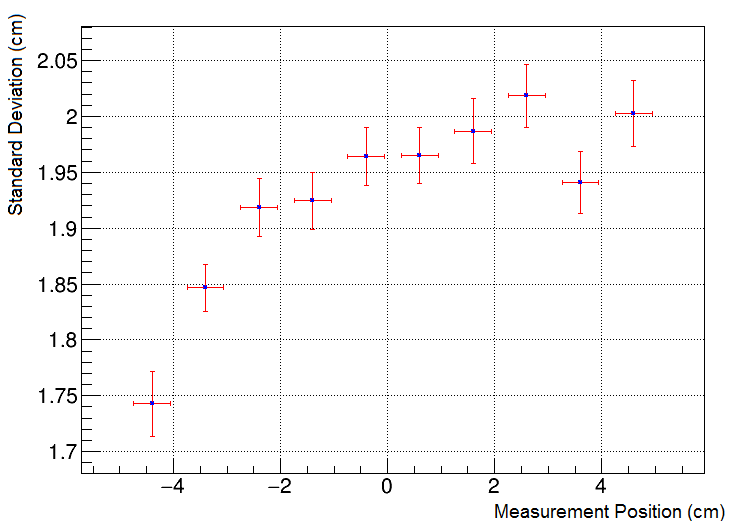
\includegraphics[width=120mm,scale=2.0]{figures/pro2.png} \caption{Standard deviation to measurement position. Here one can see the standard deviations of the calibrated measurements.}  \label{fig:pro2}\end{figure}
Figure \ref{fig:pro3} shows the systematic errors together with statistical errors which are presented in Figure \ref{fig:pro2}.
\begin{figure}[] \hspace*{-0cm} 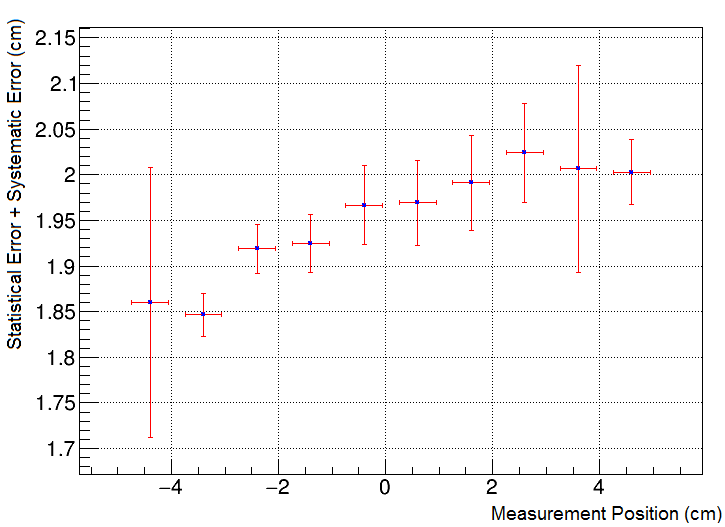
\includegraphics[width=120mm,scale=2.0]{figures/pro3.png} \caption{Here the systematic errors are presented together with the statistical errors.} \label{fig:pro3}\end{figure}
\\In Figure \ref{fig:pro4} one can see how the Gaussian fits of the measurements overlap.
\begin{figure}[] \hspace*{-0cm} 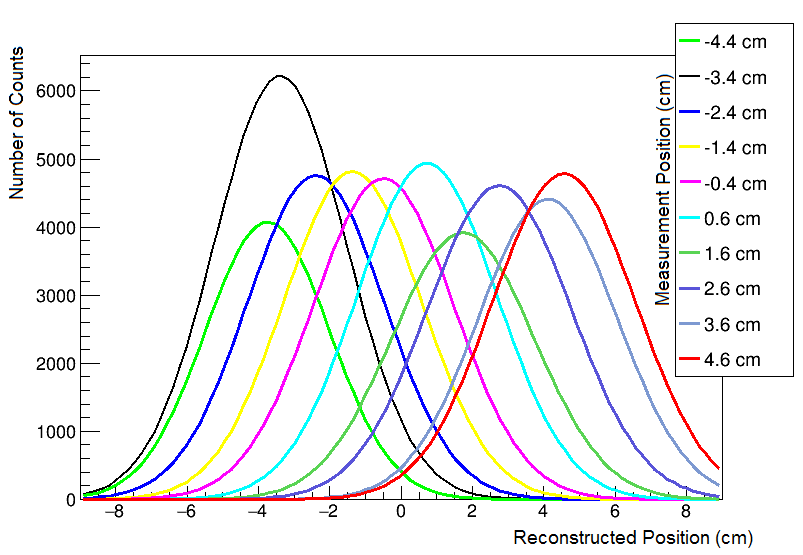
\includegraphics[width=130mm,scale=2.0]{figures/pro4.png} \caption{Overlap of Gaussian fit of the calibrated measurements.}  \label{fig:pro4}\end{figure}

As it is mentioned above there is a mirror symmetry between the left and the right sides of the scintillator bar as long as there is no specific defects. 
That is why it is sensible to use the measurements which are taken at the left side as they were taken at the right side of the bar and vice versa. For example one can use the measurement which is taken at the position -3 cm as it was taken at the position 3 cm. Let us name this kind of pseudo-measurements as ``mirror measurements".
In the Figure \ref{fig:pro5} one can see the mirror measurements together with the measurements.\begin{figure}[h!] \hspace*{-0cm} 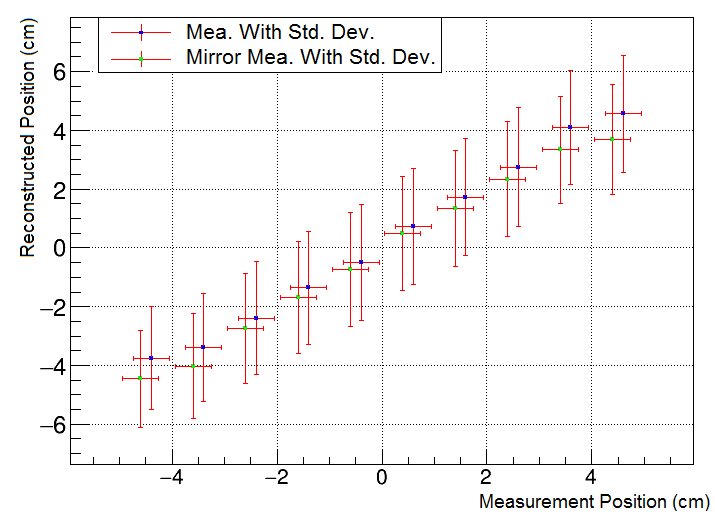
\includegraphics[width=120mm,scale=2.0]{figures/pro5.png} \caption{Measurements together with mirror measurements. The error bars with blue marker represents the measurements which are presented also in Figure \ref{fig:pro1} and the error bars with the green marker represents the mirror measurements. Here we see that the measurements support each other.} \label{fig:pro5}\end{figure}

\begin{comment}
C values of the measurements are presented in Figure \ref{fig:co}.
For the 108 mm wide bar F=0.77. In Figure  \ref{fig:calo} one can see the calibrated positions. Standard deviations of the calibrated positions are presented in Figure \ref{fig:caline}, the figure show us that we can determine position of the ionizing charged particle with maximum 1.8 cm standard deviation, this is our resolution.
\begin{figure}[h!] \hspace*{-1cm} 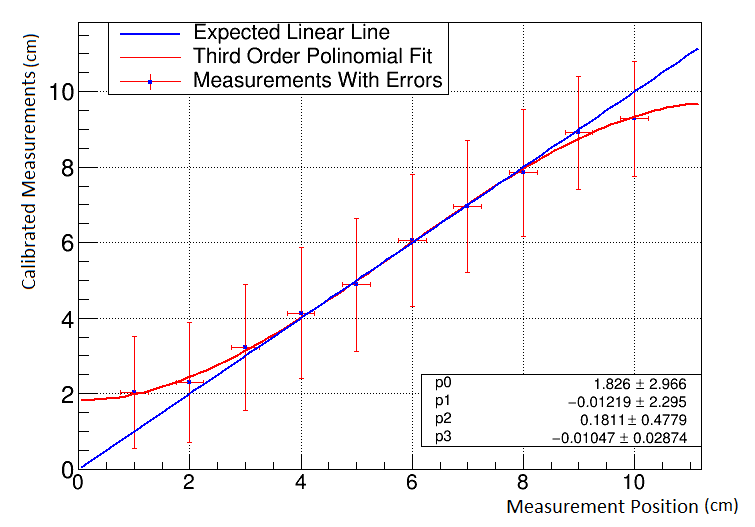
\includegraphics[width=130mm,scale=2.0]{figures/calo.png} \caption{Calibrated measurements.}  \label{fig:calo}\end{figure}
\begin{figure}[h!] \hspace*{-1cm} 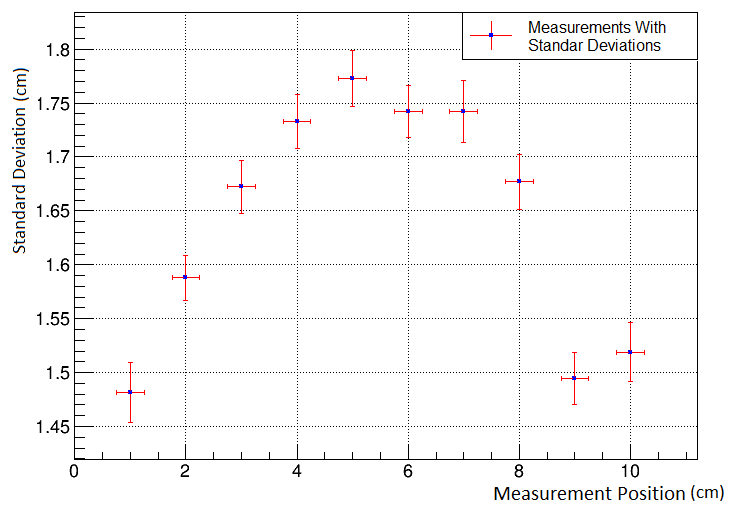
\includegraphics[width=130mm,scale=2.0]{figures/caline.png} \caption{Standard deviations of the calibrated measurements.}  \label{fig:caline}\end{figure}
In Figure \ref{fig:dist} one can see how the Gaussian fits of the measurements overlap.
\begin{figure}[h!] \hspace*{-1cm} 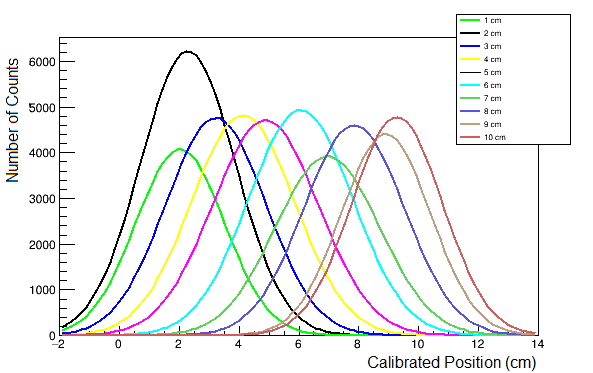
\includegraphics[width=130mm,scale=2.0]{figures/dist.png} \caption{Overlap of Gaussian fit of the calibrated positions.}  \label{fig:dist}\end{figure}

Properties of a scintillator bar should be the same at the right and left sides of its center, so, if there is no specific defects, there is a mirror symmetry between the left ad the right sides, because of this, for example, while the light travels from right fiber to left fiber, it experiences the same things as while it travels from left fiber to right fiber. That is why it is sensible to use the measurements which are taken at the left side for the right side of the bar and vice versa, let us name this kind of pseudo-measurements as "mirror measurements".
In the Figure \ref{fig:mirror} one can see the response graph after adding the mirror measurements.\begin{figure}[h!] \hspace*{-1cm} \includegraphics[width=130mm,scale=2.0]{figures/mirror.png} \caption{Calibration with mirror measurements. Here we see that the measurements support each other.} \label{fig:mirror}\end{figure}
\end{comment}

\subsection{Measurements with 59.5 mm-wide Bars} 
This is the slimmest scintillator bar used in the CRT modules. The size of the modules used in the measurements is $0.96 \times 2.72$ $\mathrm{m^{2}}$. As it is mentioned in Section \ref{chap:mu}, for 59.5 mm wide scintillator bars the optimized attenuation length is $\lambda=10.5\pm2$~cm.
\\By using three $0.96 \times 2.72$ $\mathrm{m^{2}}$ CRT modules, the measurements was made at 80 and 220 cm from the readout end. Serial numbers of the modules are 372, 373 and 374. In Appendix \ref{App:AppendixB} one can find the measurement details, like at which position, for how many hours the measurements run, for the measurements at 80 cm from the readout end.

\subsubsection{Module 372} 
In Figure \ref{fig:72m} one can see the reconstructed positions versus the measurement positions at 80 cm from the readout end for the module which has the serial number of 372.
\begin{figure}[h!] \hspace*{-0cm} \includegraphics[width=120mm,scale=2.0]{figures/72m.png} \caption{Calibrated measurements for the module 372 at 80 cm from the readout end.}  \label{fig:72m}\end{figure}
The standard deviations of the measurements can be seen in Figure \ref{fig:72s}.
\begin{figure}[h!] \hspace*{-0cm} \includegraphics[width=120mm,scale=2.0]{figures/72s.png} \caption{Standard deviation of the measurements with the module 372 at 80 cm from the readout end.}  \label{fig:72s}\end{figure}
Sum of the systematic errors and the statistical errors can be seen in Figure \ref{fig:72e}.
\begin{figure}[h!] \hspace*{-0cm} \includegraphics[width=120mm,scale=2.0]{figures/72e.png} \caption{Total error of the measurements with the module 372 at 80 cm from the readout end.}  \label{fig:72e}\end{figure}
\\The mirror measurements can be seen in Figure \ref{fig:72mir}.
\begin{figure}[h!] \hspace*{-0cm} \includegraphics[width=120mm,scale=2.0]{figures/72mir.png} \caption{Measurements together with the mirror measurements for the module which has serial number 372 at 80 cm from the readout end. Here we see that the measurements are compatible with each other.}  \label{fig:72mir}\end{figure}

For this module the results at 220 cm from the readout end can be seen in Figure \ref{fig:72fm}, Figure \ref{fig:72fs} and Figure \ref{fig:72fe}. 
\begin{figure}[h!] \hspace*{-0cm} \includegraphics[width=120mm,scale=2.0]{figures/72fm.png} \caption{Calibrated measurements for the module 372 at 220 cm from the readout end.}  \label{fig:72fm}\end{figure}
\begin{figure}[h!] \hspace*{-0cm} \includegraphics[width=120mm,scale=2.0]{figures/72fs.png} \caption{Standard deviation of the measurements with the module 372 at 220 cm from the readout end.}  \label{fig:72fs}\end{figure}
\begin{figure}[h!] \hspace*{-0cm} \includegraphics[width=120mm,scale=2.0]{figures/72fe.png} \caption{Total error of the measurements with the module 372 at 220 cm from the readout end.}  \label{fig:72fe}\end{figure}

\subsubsection{Module 373} 
Since the measurement results of the 3 modules are similar, for the modules which have serial number 373 and 374 only the standard deviation to true position and the total error graphs will be shared.

For the measurements at 80 cm from the readout end, standard deviation of the measurements can be seen in Figure \ref{fig:73s}. Total error of the measurements are in Figure \ref{fig:73e}. 
\begin{figure}[h!] \hspace*{-0cm} \includegraphics[width=120mm,scale=2.0]{figures/73s.png} \caption{Standard deviation of the measurements with the module 373 at 80 cm from the readout end.}  \label{fig:73s}\end{figure}
\begin{figure}[h!] \hspace*{-0cm} \includegraphics[width=120mm,scale=2.0]{figures/73e.png} \caption{Total error of the measurements with the module 373 at 80 cm from the readout end.}  \label{fig:73e}\end{figure}

For the measurements at 220 cm from the readout end, the standard deviation of the measurements can be seen in Figure \ref{fig:73fs} and their total error is in Figure \ref{fig:73fe}.
\begin{figure}[h!] \hspace*{-0cm} \includegraphics[width=120mm,scale=2.0]{figures/73fs.png} \caption{Standard deviation of the measurements with the module 373 at 220 cm from the readout end.}  \label{fig:73fs}\end{figure}
\begin{figure}[h!] \hspace*{-0cm} \includegraphics[width=120mm,scale=2.0]{figures/73fe.png} \caption{Total error of the measurements with the module 373 at 220 cm from the readout end.}  \label{fig:73fe}\end{figure}

\subsubsection{Module 374} 
For the module which has serial number 374, standard deviation and the total error of the measurements at 80 cm from the readout end can be seen in Figure \ref{fig:74s} and Figure \ref{fig:74e}.
\begin{figure}[h!] \hspace*{-0cm} \includegraphics[width=120mm,scale=2.0]{figures/74s.png} \caption{Standard deviation of the measurements with the module 374 at 80 cm from the readout end.}  \label{fig:74s}\end{figure}
\begin{figure}[h!] \hspace*{-0cm} \includegraphics[width=120mm,scale=2.0]{figures/74e.png} \caption{Total error of the measurements with the module 374 at 80 cm from the readout end.}  \label{fig:74e}\end{figure}

For this module, measurements were taken only at 80 cm from the readout end.

\subsection{Measurement Results}
\label{chap:exres} 
ADC output of an event is formalized as
\begin{equation} \label{eq:adc} ADC = P + G~\kappa~n_{\gamma}, \end{equation}
where $P$ is pedestal, $G$ is gain of the MPPC, $\kappa$ is conversion parameter from photon to electron and $n_{\gamma}$ is number of the photons reached to the MPPC.
\\Via Equation \ref{eq:i1i2} and Equation \ref{eq:pos}, for $L=108$~mm wide bars the reconstructed position, in cm unit, can be written as
\begin{equation} \label{eq:pos1} r_{1}=\frac{1}{2} \Big(10.8 - 7.9~ln(\frac{ADC_{1} - P_{1} }{ADC_{2} - P_{2}} ~\frac{G_{2}}{G_{1}})\Big) . \end{equation}
For $L=59.5$~mm wide bars the reconstructed position, in cm unit, is
\begin{equation} \label{eq:poss2} r_{1}=\frac{1}{2} \Big(5.95 - 10.5~ln(\frac{ADC_{1} - P_{1} }{ADC_{2} - P_{2}} ~\frac{G_{2}}{G_{1}})\Big) . \end{equation}
%For $L=108$~mm wide bars the optimal attenuation length $\lambda=1/\mu=7.9\pm1$~cm and for $L=59.5$~mm wide bars $\lambda=1/\mu=10.5\pm2$~cm.
\\By using Equation \ref{eq:pos1}, for 108 mm wide bars, one can determine position of a muon with maximum 1.9 cm average spatial resolution.
%, where standard deviation of the equal distribution is 3.12 cm. 
For the 59.5 mm wide bars Equation \ref{eq:poss2} gives 1.93 cm average spatial resolution.
%, where standard deviation of the equal distribution is 1.72 cm.

A better resolution leads to minimize the loss of the fiducial volume cut due to crossing cosmic rays.
Let us think that a cosmic muon passed through a 108~mm wide scintillator bar and interacted with the LAr inside the TPC, see Figure \ref{fig:cmp}. 
A photon which is created in the interaction of the cosmic muon with the LAr can produce a signal which can be mistaken with a neutrino interaction. This is why one has to remove a cylindrical volume which should minimum have radius of conversion length of the photon in the LAr, 18 cm, around the muon track. If one wants to remove a 20~cm radius cylindrical volume around the muon track, in case of $10.8/\sqrt{12}$ cm spatial resolution, the radius of the cylinder would be 23.12 cm, in Figure \ref{fig:cmp} this is represented with $r_{1}$, in case of 1.9 cm spatial resolution the radius would be 21.9~cm, which is represented with $r_{2}$ in the figure. 
1.9~cm resolution leads to $19.1~\%$ less loss of the fiducial volume than $10.8/\sqrt{12}$ cm resolution. By maximizing the fiducial volume, the CRT leads to a better detection sensitivity of the TPC to neutrino measurements.
\begin{figure}[h!] \hspace*{1.2cm} \includegraphics[width=90mm,scale=2.0]{figures/cmp.png} \caption{A photon which is created in the interaction of the cosmic muon with the LAr can create a signal which can be mistaken with a neutrino interaction. This is why one has to remove a cylindrical volume around the muon track. A better resolution corresponds to smaller radius of the cylinder and therefore leads to less loss of the fiducial volume.}  \label{fig:cmp}\end{figure}

%\subsection{Measurement \RNum{2}}
%I placed 3 ?? (cm) x ?? (cm) CRTs between the PMTs as you can see in figure ?(zeten koydugum) The distance between 2 PMTs is $26$ $cm$ a4
%Lateral surfaces of the CRTs are not parallel to each other, they are slightly shifted, at the front left side- FEB's left side, the second CRT (serial number 366) is not shifted respect the the first CRT (serial number 368) but the third CRT (serial number 365) is 1 mm shifted respect the the first CRT. At the beginning of the PMTs, in the figure ? left side, the second CRT is 1.15 mm shifted respect the the first CRT (serial number 368) and the third CRT (serial number 365) is 1.56 mm shifted respect the the first CRT. Burada anlattigim olay thin modul ile yaptigimiz ilk deney, sonra onu iptal etmistik zaten number of counts dusuk diye. Tezde koydugun measurementlerde boyle bi sikinti yok.
%(BURAYA BI TEKNIK CIZIM)

%%%%%%%%%%%%%%%%%%%%%%%%%%%%%%%%%%%%%%%%%%%%%%%%%%%%%
\clearpage
\newpage\null\thispagestyle{empty}
\subsection{Variables of Position Measurement}
\label{chap:temp}

During the measurements, it is not possible to correct all the effects influencing the position measurements. 
%During the measurements, it is not possible to continuously keep track of all the variables which can affect the position measurements. 
This section presents how the change in some parameters of ADC affects the reconstructed position of a charged particle.
%As it is mentioned in Section \ref{chap:exres}, ADC output of an event is formalized as  $ADC~=~P~+~G~\kappa~n_{\gamma}$. 
\\The gain of an MPPC is sensitive to ambient temperature. In the following, starting from the gain measurement of an MPPC and gain fluctuations due to temperature changes, the effect of gain variation on the position measurements is presented.

\subsubsection{Effect of Gain Variation}
\label{chap:gdf}
To measure the gain of an MPPC one needs to measure its spectrum, see Figure~\ref{fig:cp}, and calculate the distance between the photonpeaks.
In Figure \ref{fig:gain} the gain is the slope of the red line.%, since the errors of the peaks are very small it is not possible to see them in this figure, they are plotted in Figure \ref{fig:gaine}
\begin{figure}[] \hspace*{-1cm} \includegraphics[width=130mm,scale=2.0]{figures/gain.png} \caption{The gain is the slope of the red line. Since the errors of the peaks are very small it is not possible to see them in this figure, they are plotted in Figure \ref{fig:gaine}. For the photonpeaks see Figure \ref{fig:cp}.} \label{fig:gain}\end{figure}
\begin{figure}[] \hspace*{-1cm} \includegraphics[width=130mm,scale=2.0]{figures/gaine.png} \caption{Errors of the photonpeaks in Figure \ref{fig:gain}.} \label{fig:gaine}\end{figure}

In order to see if there is a significant fluctuation in the gains of the MPPCs due to temperature changes, gains of two MPPCs which are placed in a $0.96 \times 2.72$ $\mathrm{m^{2}}$ CRT module were measured at the module temperatures of 20.8, 24.2, 25, 27 and 27.4 $C^{\circ}$. Serial number of the CRT module used in these measurements is 372.
The temperature was measured using a 0.1 $C^{\circ}$ precise digital thermometer, see Figure \ref{fig:term}.
\begin{figure}[] \centering \includegraphics[width=70mm,scale=1.0]{figures/termpaint.png} \caption{To measure the temperature a digital thermometer is placed on top of the module over the regarded scintillation bar.} \label{fig:term} \end{figure}  
Prior to the measurement the ambient temperature was almost constant for at least 1 hour. As it can be seen Figure~\ref{fig:rvsm}, the temperature of the module is more stable than the temperature of the ambient. 
Total change in the ambient temperature is $8.1~C^{\circ}$ while the total temperature change in the module is $6.4~C^{\circ}$.
\begin{figure}[] \centering \includegraphics[width=130mm,scale=1.0]{figures/mea.png} \caption{Correlation between the room temperature and the module temperature.} \label{fig:rvsm} \end{figure}  
\\In Figure \ref{fig:mea} one can see how the gain of the MPPCs changes with temperature. It is clear that the gain decreases with the temperature increase. This is because, although capacitance of the MPPC increases \cite{123}, increasing of temperature leads to greater breakdown voltage \cite{1234} and thus lowers the gain.
\begin{figure}[] \centering \includegraphics[width=130mm,scale=1.0]{figures/rvsm.png} \caption{Gain change versus module temperature change. "Channel 0"  represents the first channel's MPPC and "Channel 1" the second ones. The gain change of Channel 1 is less than the change of Channel 0. This is because the latter one is closer to the corner of the module such that the change in the room temperature affects it more.} \label{fig:mea} \end{figure}  

The method which is used for the position calculation is affected by change in the ratio of the gains than absolute gain changes. The change of the gain ratios with the temperature is shown in Figure \ref{fig:ratio}. At 27~$C^{\circ}$ Channel 0 has an outlier, if one neglects the outlier, the ratio of the maximum gain-ratio to the minimum gain-ratio is 1.065.
 \begin{figure}[] \centering \includegraphics[width=130mm,scale=1.0]{figures/ratiot.png} \caption{Ratio of the gains, $Gain_{Ch0}$/$Gain_{Ch1}$, versus temperature.} \label{fig:ratio} \end{figure}  
%The room at FermiLab where the CRT modules are located, is kept at a constant temperature within $2~C^{\circ}$. This temperature change will affect the position measurements as a systematic error.

If the ratio of the gains change with a factor of C, $\frac{G_{2}}{G_{1}} \to \frac{C\ G_{2}}{G_{1}}$, this change shows itself as an offset in the reconstructed position;
%\begin{equation} \label{eq:pos} r_{1}^{'}=\frac{1}{2} \Big(L - \frac{1}{2\mu} ln(\frac{ADC_{1} - ped_{1} }{ADC_{2} - ped_{2}}) - \frac{1}{2\mu} ln(\frac{gain_{2}}{gain_{1}} )- \frac{1}{2\mu} ln(C)\Big) \end{equation}
\begin{equation}r_{1}^{'}=r_{1} - \frac{1}{2\mu} ln(C) . \end{equation}
\\If one increases the gain of Channel 1 by $15\%$ in the measurements presented in Section \ref{chap:108mm}, at the average the mean values of the reconstructed positions differ 0.27 cm from the values derived via the correct gains, see Figure \ref{fig:gd}.
\begin{figure}[] \hspace*{-1cm} \includegraphics[width=130mm,scale=1.0]{figures/gd.png} \caption{If one changes the gain of Channel 1 $15\%$ in the measurements presented in Section \ref{chap:108mm}, at the average the mean values of the reconstructed positions differ 0.27 cm from the values derived via the correct gains.} \label{fig:gd} \end{figure}  
In Figure \ref{fig:gdp} one can see how the average mean value of the reconstructed positions changes if one increases the value of the first channel's gain from 100 percent to 200 percent.
\begin{figure}[] \hspace*{-1cm} \includegraphics[width=130mm,scale=1.0]{figures/gdp.png} \caption{Here one can see how the average mean value of the reconstructed positions changes if one increases the value of the first channel's gain from 100 percent to 200 percent.} \label{fig:gdp} \end{figure}  

Number of the muons which interact with the CRT modules is equally distributed. %right? top and bottom okay but others?
But because of the reflections from the corners it is not possible to see an equal distribution at the measurements. 
If one compares the reconstructed positions with the real positions, the reconstructed positions look like squeezed with respect to real positions, Figure \ref{fig:pro1} and Figure \ref{fig:72m} can be helpful to see this effect. 
As it is mentioned above the deviation in the ratio of the gains shifts the reconstructed positions. 
%Since all of the measurements shift, by looking at the number of the events at middle region of the scintillator bar, one cannot understand if the gains need to be calibrated. 
Although the number of the measured muons at the corner regions is less than the middle region, one can expect to see the same number of the detected muons on the two corner regions. 
By comparing the number of the detected muons on the two corner regions of the bar, one can understand if the measurements are shifted and gain calibration is needed. 

%Let us say ``left region" for the region which starts from the left corner and goes 2 cm toward the middle of the bar, ``right region" for the similar right side and think that left region detected 100 events while the right region detected 120 events.Above we saw that when the ratio of the gains change $15\%$, the mean values of the calculated positions shift 0.27 cm. If one creates a histogram with 0.01 cm bin size and at the middle region each bin has 2 events, 120-100=20, 20*0.01/2=0.1. This means that there is a change in the gain such that is creates 0.1 cm shifting and shold be calibrated. Now we go, look at the graph which i will draw and see how much we should change the gains. Also see the figure gd in the thin bars to see if the symmetric behavior still exists.....

Via Equation \ref{eq:adc} one can see that when there is a deviation in the number of the photons reached to an MPPC or a deviation in the $\kappa$ conversion parameter of an MPPC this would create a similar effect as the change in the gains and therefore it can be calibrated in the same way as described above.

\subsubsection{Effect of Pedestal Variation}
Let us assume that in Equitation \ref{eq:pos1} the $P_{1}$ increased with a value of V, $P_{1}\to P_{1}+V$. 
In this case the reconstructed position can be written as
\begin{equation} \label{eq:pos2} r_{1}=\frac{1}{2} \Big(L - \frac{1}{\mu} ln(\frac{ADC_{1} - P_{1} }{ADC_{2} - P_{2}}+\frac{ V }{ADC_{2} - P_{2}}) - \frac{1}{\mu} ln(\frac{G_{2}}{G_{1}})\Big) . \end{equation}
Here we see that effect of the increment parameter $V$ is proportional with the other channel's ADC and pedestal values. Unlike the change in the ratio of the gains, change of a pedestal leads to an antisymmetric effect.
\\When one increases the pedestal of Channel 1 $15\%$ in the measurements presented in Section \ref{chap:108mm}, the antisymmetric effect can be clearly seen as it is presented in Figure~\ref{fig:pedc}.
\begin{figure}[h!] \hspace*{-1cm} \includegraphics[width=130mm,scale=2.0]{figures/pedc.png} \caption{$15\%$ increasing of  the pedestal of Channel 1 in the measurements presented in Section \ref{chap:108mm}. This change creates an antisymmetric effect.}  \label{fig:pedc}\end{figure}
\\Since the pedestal is not very sensitive to the ambient temperature and those changes do not create a significant effect on accuracy of the measurements, 
a calibration process for the pedestal will not be described here.

\subsubsection{Effect of Reflective Surface}
\label{chap:ref}
As it is mentioned in Section \ref{chap:gdf} a change in the number of the photons reached the MPPC would create a similar effect as the change in the gains. Let us assume that the number of the photos reached the MPCCs decreased in a way that this decrease did not create a net effect in Equation \ref{eq:pos2}, what would chance with the reconstructed positions?
In order to answer this question and reveal the effect of the internal reflection on the position measurements, a 11.2 cm wide, 50 cm long single-bar CRT module is built, see Figure \ref{fig:small}.
\begin{figure}[] \centering \includegraphics[width=120mm,scale=1.0]{figures/small.jpg} \caption{A 11.2 cm wide, 50 cm long single bar-CRT module with its connector.} \label{fig:small} \end{figure}  
By using a muon telescope, as it is described in Chapter \ref{chap:measurements}, at 7 different positions measurements are taken and after removing the chemically modified white surface of the bar the measurements has been repeated, see Figure \ref{fig:trans}.
\begin{figure}[h!] \centering \includegraphics[width=100mm,scale=1.0]{figures/trapaint.png} \caption{On the left side one can see how the scintillator bar looks like, and on the right side after removing its white surface. The white surface of the bar has been removed by using rasp parer, that is why the surface has a lot of scratches which reduce its transparency.} \label{fig:trans} \end{figure}  

Measurements showed that the white surface on the bar increases the internal reflectivity which leads to more light collection by the fibers, see Figure \ref{fig:s0ps1}. Standard deviation of those measurements are presented in Figure \ref{fig:s0ps1e}.
\begin{figure}[] \centering \includegraphics[width=120mm,scale=1.0]{figures/s0ps1.png} \caption{Vertical axis is the total number of the photonelectrons in the two MPPCs of the bar. ``0" on the horizontal axis represents the middle of the bar. Here one can clearly see that the white surface on the bar leads to more light collection by the fibers.  The errors are divided by 10, one can see the standard deviations of the measurements in Figure \ref{fig:s0ps1e}.} \label{fig:s0ps1} \end{figure}  
\begin{figure}[] \centering \includegraphics[width=110mm,scale=1.0]{figures/s0ps1e.png} \caption{Standard deviations of the measurements in Figure \ref{fig:s0ps1}.}\label{fig:s0ps1e} \end{figure}  
In Figure \ref{fig:s0os1} one can see how the ratio of the number of photonelectrons in the MPCCs of the modeul decreases with and without the white surface with respect to distance. Standard deviations on this figure can be seen better in Figure \ref{fig:s0os1e}.
\begin{figure}[] \centering \includegraphics[width=120mm,scale=1.0]{figures/s0os1.png} \caption{Ratio of the photonelectrons in the two MPPCs of the bar with their exponential fits. The error bars are divided by 10, in Figure \ref{fig:s0os1e} one can see better the standard deviations on this figure.} \label{fig:s0os1} \end{figure}  
\begin{figure}[] \centering \includegraphics[width=110mm,scale=1.0]{figures/s0os1e.png} \caption{ Standard deviations of the measurements in Figure \ref{fig:s0os1}.} \label{fig:s0os1e} \end{figure}  

Removing the white surface of the scintillator bar creates the same effect on the two MPPCs of the bar which avoids to see a clear shift in the reconstructed positions, see Figure \ref{fig:rwc} .
\begin{figure}[] \centering \includegraphics[width=110mm,scale=1.0]{figures/rwc.png} \caption{Difference between the means of reconstructed positions (with and without white surface of the scintillator bar) with respect to measurement position.} \label{fig:rwc} \end{figure}  
The main effect of removing the white surface is on the standard deviations of the reconstructed positions. Since amplitude of the signals are less when there is no white surface, the relative standard deviations of the measurements are higher, the results  can be seen Figure \ref{fig:rwcc}. Thus presence of the white surface significantly improves accuracy of the measurements.
\begin{figure}[] \centering \includegraphics[width=110mm,scale=1.0]{figures/rwcc.png} \caption{In the figure one can see that after removing the white surface of the bar the, standard deviation of the reconstructed positions increase. On the right side of the graphs the measurement positions are shown. Presence of the white surface significantly improves accuracy of the measurements. (a) Reconstructed positions with white surface, (b) Reconstructed positions without white surface. } \label{fig:rwcc} \end{figure}   

%%%%%%%%%%%%%%%%%%%%%%%%%%%%%%%%%%%%%%%%%%%%%%%%%%%%%
\clearpage
\newpage\null\thispagestyle{empty}
\section{Liquid Argon Impurity Measurements via Cosmic Muons}
\label{chap:pur}
If one knows the coordinates of an ionizing particle which passes through the TPC, since the charge attenuation during the drift depends on the impurity the amount of the collected charge by the anode reveals the impurity of the LAr. In this chapter two impurity calculation procedures are illustrated for a 2-dimensional TPC.

The impurity causes exponential attenuation of the charge while it is drifted. 
If the amount of the charge created by the muon per anode wire is $Q_{0}$, the amount of the collected charge by a wire 
would be 
\begin{equation}  Q = Q_{0} \ e^{-t/ \tau}  \label{eq:pur} \end{equation}
where $t$ is the drift time till the wire and $\tau$ is lifetime of free electrons in LAr. The lifetime is related to the impurity of the LAr as $\tau\approx0.3/P$ \cite{larpur}, where $\tau$ is the life time in ms unit when $P$ is Parts Per Billion (ppb) oxygen-equivalent impurity concentration, and with respect to these units the ``0.3" in the formula gets its unit. Therefore Equation \ref{eq:pur} can be approximated as
\begin{equation}  Q = Q_{0} \ e^{-t~P/ 0.3}  \label{eq:purr1}. \end{equation}

Let us think that by passing the CRT modules the muon entered the TPC with the angle of $\theta$ to the anode axis. 
%Let us think that by passing the CRT modules the muon entered the TPC with the angle of $\theta$, from the distance $z_{i}$ to the anode and left from the distance $z_{f}$, see Figure \ref{fig:sich}.
%In the figure, $L$ is the total propagation distance of the muon in the TPC which varies from T length of the TPC to a certain $L>T$ value.
%and the propagation distance $z=z_{i}~+~L~cos\theta$. 
In this case the amount of the charge created per wire is 
\begin{equation} Q_{0}=q_{0}~l \end{equation} where $q_{0}$ is amount of the charge  created by the muon per unit length and $l~=~L/N~=~d/cos\theta$, here $L$ is the total propagation distance of the muon in the TPC, $N$ is number of the anode wires which collect the ionization charge and $d$ is the pitch distance between the wires. 
If one assumes that the charges created in the propagation distance of $l$ have the same drift distance of~$z$, Equation \ref{eq:purr1} becomes
\begin{equation} Q = q_{0}~\frac{d}{cos\theta}~e^{-t~P/ 0.3}.\end{equation} 
In this case the measured impurity concentration is
\begin{equation} P = \frac{0.3~V}{z}~\mathrm{ln}\Big(\frac{q_{0}}{Q} \frac{d}{cos\theta}\Big), \label{eq:ppb}\end{equation} 
where $z$ is the drift distance and $V$ is the drift velocity of the electron in the LAr.

Equation~\ref{eq:ppb} is a general formula which gives the value of the impurity obtained through an individual wire. Here one should take arithmetic mean of the values obtained from N anode wires.
Now let us assume that the muon entered the TPC with the angle of $\theta$, from the distance $z_{i}$ to the anode and left from the distance $z_{f}$, see Figure \ref{fig:sich}.
\begin{figure}[] \centering \includegraphics[width=100mm,scale=1.0]{figures/sich.png} \caption{Here the muon, which is represented with the red row, enters the TPC from the distance $z_{i}$ to the anode with the angle of $\theta$ to the anode axis and leaves from the distance $z_{f}$.  $L$ is the total propagation distance of the muon in the TPC, $T$ is length of the TPC and n is the number of the anode wires.} \label{fig:sich} \end{figure}  
In this case, in terms of the distances, Equation~\ref{eq:ppb} can be written as
\begin{equation} P= \frac{T~0.3~V}{T~z_{i}+d~n~(z_{f}-z_{i})}~\mathrm{ln}\Big(\frac{q_{0}}{Q_{n}}~\frac{d}{T}~\sqrt{T^{2}+z_{f}^{2}+z_{i}^{2}-2z_{f}z_{i}}\Big),\label{eq:ppbs}\end{equation} 
where $n$ is the number of the anode wire which represents the position of the wire. Here standard deviation of the impurity is
\begin{equation} \sigma_{P}= \sqrt{\sigma_{z_{i}}^2 \Big( \frac{-F~(T-dn)}{E^3} \frac{G}{2} \Big)^2 + \sigma_{z_{f}}^2 \Big( \frac{-F~dn}{E^3} \frac{G}{2} \Big)^2 + \sigma_{Q_{n}}^2 \Big( \frac{-T\ 0.3\ V}{Q_{n}\ E} \Big)^2}, \label{eq:432}\end{equation} 
where $E=T~z_{i}+d~n~(z_{f}-z_{i})$~, $F=\mathrm{ln}\Big(\frac{q_{0}}{Q_{n}}~\frac{d}{T}~\sqrt{T^{2}+z_{f}^{2}+z_{i}^{2}-2z_{f}z_{i}}\Big) 0.3 V T$ and $G=\frac{(2z_{i}-2z_{f})0.3 V T}{T^{2}+z_{f}^{2}+z_{i}^{2}-2z_{f}z_{i}}$.
\\Let us imagine that $z_{i}=40$~cm, $z_{f}=70$~cm and the number of the collected electrons in $100^{th}$ anode wire is 16000. It is known that for a minimum ionizing particle the ionization yield in LAr is 55.000~electrons/cm and the drift velocity in MicroBooNE is $\approx1.087$~m/ms \cite{1}.
Without making any calculations, with only knowing that the muon passed through the bar, for 10.8 cm wide bars the spatial resolution would be $10.8/\sqrt{12}$.
As is shown in Section \ref{chap:exres}, using the position calculation method presented in this thesis, for 10.8 cm wide bars the average spatial resolution is 1.9 cm.
This development decreases standard deviation of the measured impurity. As it was mentioned the equivalent noise in MicroBooNE is about 1000 $e^{-}$, this noise has the dominant effect on the value of the standard deviation of impurity concentration, see Equation \ref{eq:432}. To be able to see the effect of the spatial resolution development, let us assume that the equivalent noise is 0 $e^{-}$.
Under the conditions mentioned above, in case of $10.8/\sqrt{12}$ cm spatial resolution the measured impurity concentration is $P~=~24.9~\pm~1.8~\times~10^{-3}$~ppb and in case of 1.9 cm spatial resolution $P~=~24.9~\pm~1.1~\times~10^{-3}$~ppb, which means that the precision increased by $61\%$. When consider the electronic noise, in case of 1.9 cm spatial resolution the measured impurity would be $P~=~24.9~\pm~50~\times~10^{-3}$~ppb.

The impurity measurement method described above does not take into account the recombination of the ionization charge and therefore it is not the best way to follow. 
An effective way of measuring the impurity is to exponentially fit the amount of the collected charge by the wires with respect to their drift distance. Here the fitting formula is given by $f(y)=A_{0}~e^{zB_{0}}$ where $A_{0}$ and $B_{0}$ are the fit parameters. After taking into account the recombination factor $R$, in terms of drift distance Equation~\ref{eq:purr1} can be written as
\begin{equation}  Q_{n} = R~Q_{0} \ e^{-z~P/(0.3~V)}  \label{eq:purro}. \end{equation}
Therefore $A_{0}=R~Q_{0}$, $B_{0}=-P/(0.3~V)$ and the impurity is $P~=~-B_{0}(0.3~V)$.
Following this way, for the situation presented in Figure~\ref{fig:sich}, in terms of distances the impurity can be written as
\begin{equation}  P=\mathrm{ln}(\frac{A_{0}}{Q_{n}})~\frac{0.3\ V\ T}{Tz_{i} + (z_{f}-z_{i})d n}.  \label{eq:purrok} \end{equation}
Therefore the standard deviation of the impurity is 
\begin{equation}  \sigma_{P}=\frac{C}{D} \sqrt{\sigma_{z_{i}}^2 T^2  + \sigma_{z_{f}}^2 (dn)^2  + \sigma_{Q_{n}}^2 \Big( \frac{-0.3 \ V \ T}{ Q_{n}\ E} \Big)^2},  \label{eq:purrok} \end{equation}
where $C=\mathrm{ln}(\frac{A_{0}}{Q_{n}})~0.3 V$.
Via Equation \ref{eq:purrok} it can be seen that better spatial resolution leads to smaller error in the measured impurity of LAr.

%After calculations one can see that the total amount of the charge collected by the anode is \begin{equation} Q=Q_{T} + \frac{-q_{0} \ \tau \ e^{-z_{i}/ \tau}}{cos\theta} \Big( e^{-L\cos\theta/ \tau} -  e^{-T\cos\theta/ \tau}\Big) ,\label{eq:purl} \end{equation} where $Q_{T}=q_{0}\ T\ e^{-z_{i}/ \tau}$. In the simplest case, $z_{i}=z_{f}$ where $\theta=0^{\circ}$,  $Q=Q_{T}=q_{0}\ T\ e^{-z_{i}/ \tau}$.
%%%%%%%%%%%%%%%%%%%%%%%%%%%%%%%%%%%%%%%%%%%%%%%%%%%%%
\clearpage
\section{Conclusion}
\label{chap:concl}
%Charge collection efficiency of a bar is higher at the position nearer to the edges but the standard deviation of the values are higher there.
To gain a better understanding of $\bar{\nu}_{e}$ excess observed in the Liquid Scintillator Neutrino Detector experiment and the excess of $\nu_{e}$ and $\bar{\nu}_{e}$ events at low energy observed in MiniBooNE, the Short-Baseline Neutrino physics program is ongoing. 
The technology chosen for the SBN detectors is the LArTPC.
Since the TPCs of the SBN program are placed on the Earth surface, they are exposed to constant background of cosmic muons. This cosmic background is able to create signals inside the LArTPCs, which could be misidentified as neutrino interactions. This undesired situation will be mitigated by the CRT system developed in Bern.
%The CRT system developed in order to reject cosmic background in SBN program.
%The optimal linear attenuation coefficient is $\mu=7.9\pm1$~$cm^{-1}$ for 108 mm wide scintillator bars and $\mu=10.5\pm2$~$cm^{-1}$ for 59.5 mm wide bars.
\\As I presented in Chapter \ref{chap:crt}, the CRT system consists of CRT modules which are a combination of plastic scintillator with wavelength shifter fibers connected to multi-pixel photo counters and a readout system.

I derived the transverse position of a charged particle crossing a scintillator bar from the ratio of the created scintillation light signals at the opposite sides of the bar by using exponential photon absorption process. The calculation procedure can be found in Chapter \ref{chap:pdc}.
For 10.8 cm wide bars the position of a charged ionizing particle can be determined with 1.9 cm average spatial resolution. For 5.95 cm wide bars the average spatial resolution is 1.93 cm, the measurement results are presented in Chapter \ref{chap:measurements}. 
Maximizing the resolution of the CRT modules 
leads the loss of fiducial volume in the LArTPCs due to cut for crossing cosmic rays to be minimized.
%For 5.95 cm wide bars, the average spatial resolution is 1.93 cm. The resolution is lower because being closer to the corners gives higher standard deviation in the measurements and, since the propagation distance is lower, the amplitude difference between the two signals which lead to better position determination is lower.
\\While the CRT system is operating, it is not possible to continuously keep track of all the variables which can affect the reconstructed positions, like gain of the MPPCs.
In Section \ref{chap:temp} I showed that the gain of an MPPC is sensitive to the ambient temperature.
A change in the ratio of the gains of pair MPPCs shows itself as an offset in the reconstructed positions. 
In the range of 19~$C^{\circ}$ to 27.1~$C^{\circ}$ ambient temperature, the reconstructed positions shift by a maximum of 0.33 cm. 
During the measurements this effect should be taken into account as a systematic error. 
\\Pedestal of the MPPCs does not have a significant dependence on the ambient temperature. Those changes of the pedestal does not create significant effect on accuracy of the measurements.
%When the room temperature changes $8.1~C^{\circ}$, the temperature of the CRT module changes $6.4~C^{\circ}$ and the ratio of the gain of two MPPCs of the scintillator bar changes $25~\%$. 
\\The surface of the scintillator bars are chemically modified to increase the internal reflectivity.
Aging can cause decrease in the internal reflectivity of the scintillator bars. As is presented in Section \ref{chap:ref}, I made a set of measurements to reveal effect of the internal reflectivity on the reconstructed positions.
In a 11.2 cm wide scintillator bar, the white coating around the bar leads to $1.80~\pm~0.05$ times more light collection by the fibers and significantly improves accuracy of the measurements.
The measurements in Section \ref{chap:temp} also show that production of the CRT modules should be made very carefully because any imperfections, like impurities on the way of photons, can cause a deviation on the reconstructed position of the cosmic muons.

In Chapter \ref{chap:pur} I presented that by using the through going cosmic ray muons one can measure the impurity concentration of LAr inside the active volume of the TPC. Via the position calculation method presented in this thesis, the precision of the measured impurity increases. 
The equivalent noise in MicroBooNE is about 1000 $e^{-}$ and this noise has the dominant effect on the standard deviation of the impurity concentration measurements. Under this relatively high equivalent noise, for the impurity measurements, my spatial resolution development loses its importance.
% by $39.3\%$ compared to the impurity obtained by using $10.8/\sqrt{12}$ cm spatial resolution.

Conversion length of the photon in the LAr is 18 cm, if one wants to cut a 20 cm radius volume around the cosmic muon track, via the position calculation method described in this thesis the loss of the fiducial volume due to cut is reduced by $19.1~\%$ for 10.8 cm wide bars. 
Increasing the fiducial volume is important to obtain a good detection sensitivity to neutrino interactions.
%By maximizing the fiducial volume, the CRT increases the detection sensitivity of the TPC to neutrino measurements.

%Also, during the measurements we have seen that the CRT modules are sensitive to vibrations. The base where they stay on should be stable.

%%%%%%%%%%%%%%%%%%%%%%%%%%%%%%%%%%%%%%%%%%%%%%%%%%%%%
\clearpage

\begin{thebibliography}{9}
%\cite{B}

\bibitem{E} 
I. Kreslo, M. Auger, D. Lorca.
\textit{SBND Cosmic Ray Tracker Design and Performance Technical Note}. 
November 15, 2015.

\bibitem{vcx}
Y. Fukuda et al. (Super-Kamiokande Collaboration).
\textit{Evidence for Oscillation of Atmospheric Neutrinos.}
Phys. Rev. Lett. 81, 1562. DOI:https://doi.org/10.1103/PhysRevLett.81.1562.
August 24 1998.

\bibitem{MN}
G. Karagiorgi.
\textit{Toward Solution of the MiniBooNE-LSND Anomalies} 
Nuclear Physics B - Proceedings Supplements, Volumes 229–232, August–November 2012, Pages 50-54.

\bibitem{prop}
The ICARUS-WA104 Collaboration, The LAr1-ND Collaboration, The MicroBooNE Collaboration, Additional Fermilab Contributors.
\textit{A Proposal for a Three Detector Short-Baseline Neutrino Oscillation Program in the Fermilab Booster Neutrino Beam.}
ArXiv:1503.01520v1.
March 5 2015
%https://arxiv.org/pdf/1503.01520v1.pdf

\bibitem{K} 
FermiLab Today. MiniBooNE reports.
\url{http://www.fnal.gov/pub/today/SpecialROWMiniBooNE121208.html}. 
\today.

\bibitem{KP}  %6
A. A. Aguilar-Arevalo et al. (MiniBooNE Collaboration).
\textit{Improved Search for $\bar{\nu_{\mu}} \to \bar{\nu_{e}}$ Oscillations in the MiniBooNE Experiment}.
Phys. Rev. Lett. 110, 161801. April 15, 2013.

\bibitem{LK}
C. Adams (Yale U.) et al.
\textit{LAr1-ND: Testing Neutrino Anomalies with Multiple LArTPC Detectors at Fermilab}.
ArXiv: 1309.7987v3. 
November 5 2013

\bibitem{mic}
R. Acciarri et al.
\textit{First Observation of Low Energy Electron Neutrinos in a Liquid Argon Time Projection Chamber.}
ArXiv: 1610.04102v1.
October 13 2016.
 
\bibitem{PP}
MicroBooNE Collaboration, MicroBooNE Public Notes Page.
\textit{MicroBooNE-NOTE-1019-PUB Convolutional Neural Networks Applied to Neutrino Events in a Liquid Argon Time Projection Chamber}.
July 4, 2016.

\bibitem{NKR} %10
Q. He, K. T. McDonald. 
\textit{Electron Drift Velocity in the $\mu$BooNE TPC}
Joseph Henry Laboratories, Princeton University, Princeton, NJ 08544.
\url{http://puhep1.princeton.edu/~kirkmcd/microBooNE/KTM/DriftV.pdf}.
March 20, 2009.

\bibitem{1}
A. Schukraft.  
\textit{The Fermilab Short-Baseline Program: MicroBooNE talks in JPS Conference Proceedings, Volume 12} December 13, 2016.

\bibitem{muos}
K. Nakamura et al. (Particle Data Group). 
\textit{COSMIC RAYS}.
J. Phys. G 37, 075021 (2010)  and 2011 partial update for the 2012 edition. 
http://pdg.lbl.gov/2011/reviews/rpp2011-rev-cosmic-rays.pdf


\bibitem{C} 
MANUFACTURER: UNIPLAST Inc. 
Material Safety Data Sheet.
\textit{USMS-03 Scintillating Plastic}. 
MSDS DATE: 12.01.20014.

\bibitem{D} 
Kurray, Wavelength shifting fibers.
\url{http://kuraraypsf.jp/psf/ws.html}. 
\today.

\bibitem{hama} 
Private commutation with Hamamatsu.

\bibitem{csda} 
National Institute of Standards And Technology.
\url{http://physics.nist.gov/PhysRefData/Star/Text/ESTAR.html}. 
\today.

\bibitem{omega}
Omega microelectronics.
\url{https://indico.cern.ch/event/192695/contributions/353181/attachments/277133/387721/Citiroc_ASIC.pdf}.
\today.



%\bibitem{F} 
%\url{figures/http://www.nuclear-power.net/wp-content/uploads/2015/03/attenuation.png}. 

%\bibitem{G} 
%Electromagnetic showers.
%\url{http://www-cdf.fnal.gov/~group/WORK/DISS_PAGE/EM_SHOWER.gif}. 
%\today.

%\bibitem{L} 
%Elementary particles.
%\url{https://upload.wikimedia.org/wikipedia/commons/1/1c/Standard_Model_of_Elementary_Particles-de.svg}. 
%\today.

%\bibitem{M} 
%\url{figures/http://i.stack.imgur.com/REs1a.png}. 

%\bibitem{N} 
%\url{http://hep.bu.edu/~superk/cherenkov.gif}. 

%\bibitem{KN} 
%The MiniBooNE Experiment
%H. Ray
%Los Alamos National Laboratory, USA



%\bibitem{LL}
%The ALEPH, DELPHI, L3, OPAL, SLD Collaborations, the LEP Electroweak Working Group, the SLD Electroweak and Heavy Flavour Groups.
%\textit{Precision Electroweak Measurements on the Z Resonance}.
%ArXiv: hep-ex/0509008v3.
%February 27 2006.

%\bibitem{KM}
%FermiLab Today. Horn.
%\url{figures/http://www.fnal.gov/pub/today/archive/archive_2015/images/horn-03-0216-25D.jpg}.
%\today.

%\bibitem{PK}
%arxiv.org/pdf/1101.2755v4.pdf

%\bibitem{PR}
%\textit{The MiniBooNE Neutrino Beam and the Magnetic Focusing Horn.}
%\url{http://home.fnal.gov/~sorel/beamlinehornchapter.pdf}
%\today.



%\bibitem{MP}
%B. Jones. MicroBooNE talks.
%\textit{Introduction to Scintillation Light in Liquid Argon.}.
%\url{http://www-microboone.fnal.gov/talks/LArTPCWorkshopScintLight_bjpjone_2014.pdf}

%\bibitem{MR}
%Teppei Katori.  MicroBooNE talks.
%\textit{MicroBooNE, A Liquid Argon Time Projection Chamber (LArTPC) Neutrino Experiment}
%ArXiv:1107.5112v1. 
%July 26 2011

%\bibitem{MSD}
%F. Reines, C.L. Cowan. 
%\textit{The Neutrino}. 
%Nature. 178 (4531): 446. DOI:10.1038/178446a0.
%September 1 , 1956.

%\bibitem{MNR}
%J. Zennamo.
%\textit{The Short-Baseline Neutrino Program}.
%\url{http://microboone-docdb.fnal.gov/cgi-bin/RetrieveFile?docid=4431&filename=Zennamo_SBN_UsersMeeting.pdf&version=5}

%\bibitem{R}
%T. Briese, L. Bugel et. al.
%\textit{Testing of Cryogenic Photomultiplier Tubes for the MicroBooNE Experiment}.
%ArXiv:1304.0821v4.
%June 17 2013.





%\bibitem{1}
%A. Schukraft.  MicroBooNE talks.
%\textit{The Fermilab Short-Baseline Program: MicroBooNE}.
%\url{http://microboone-docdb.fnal.gov/cgi-bin/RetrieveFile?docid=6090&filename=nuint2015-%proceedings.pdf&version=1}.
%February 7-13, 2016.

%\bibitem{Pak}
%W. Pauli. 
%\textit{Letter, addressed to participants of the Tubingen conference on radioactivity. }
%Available from the CERN Document server:
%\url{http://cdsweb.cern.ch/record/83282P}. 
%December 1930.

%\bibitem{Cdw}
%J. Chadwick. 
%\textit{Possible existence of a neutron.} 
%Nature, 129(312), 1932.

%\bibitem{Bok}
%E. Fermi. 
%\textit{Towards the theory of $\beta$-rays.} 
%Z. Phys, 88(161), 1934.

%\bibitem{mudi}
%G. Danby, J. Gaillard, K.Goulianos, L. Lederman, N. Mistry, and M.Schwartz. 
%\textit{Observation of high-energy neutrino reactions and the existence of two kinds of neutrinos.} 
%Phys. Rev. Lett., 9(1), 1962.

%\bibitem{tud}
%M. Perl and et al. 
%\textit{Evidence for anomalous lepton production in electron positron annihilation.} 
%Phys. Rev. Lett., 35(22):1489-1492, Dec 1975.

%\bibitem{rdj}
%R. Davis, D. Harmer, and K. Hoffman. Search for neutrinos from the sun. Phys.
%Rev. Lett., 20:1205-1209, 1968.

%\bibitem{taud}
%K. Kodama and et al. 
%\textit{Observation of tau neutrino interactions.} 
%Phys. Lett. B, 504:218-224, 2001.

%\bibitem{imbk}
%G.L. Fogli, E. Lisi.
%\textit{On the Atmospheric Neutrino Anomaly and its Statistical Significance}.
%Phys.Rev. D52 (1995) 2775-2782. DOI: 10.1103/PhysRevD.52.2775.
%April 1995.

%\bibitem{SDP}
%\textit{News from MicroBooNE, December 2013.}
%\url{http://www2.lns.mit.edu/~conrad/newsDec2013.html}.
%\today.

%\bibitem{zukf}
%Y. Fukuda and et al. Study of the atmospheric neutrino flux in the multi-GeV energy range. Phys. Lett. B, 436:33-41, 1998.

%\bibitem{sno}
%Q. Ahmad and et al. 
%\textit{Direct evidence for neutrino flavor transformation from neutral-current interactions in the Sudbury Neutrino Observatory.} 
%Phys. Rev. Lett., 89(011301), 2002

%\bibitem{smm}
%M. Goldhaber, L. Grodzins, and A. W. Sunyar. 
%\textit{Helicity of Neutrinos.} 
%Phys. Rev. 109, 1015.
%February 1 1958.

%\bibitem{reno}
%Soo-B. Kim.
%\textit{Measurement of neutrino mixing angle $\theta_{13}$ and mass difference  $\Delta m_{ee}^{2}$ from reactor antineutrino disappearance in the RENO experiment.}
%Nuclear Physics B, Volume 908, July 2016, Pages 94–115.

%\bibitem{nost}
%P. Di Bari. 
%\textit{Some notes on neutrino physics and particle cosmology. Typeset for
%University of Southampton Neutrino Course.} 
%2013.

%\bibitem{massr}
%S. F. King.
%\textit{Neutrino Mass Models.}
%ArXiv:hep-ph/0310204v2.
%November 27 2003.

%\bibitem{conm}
%S. Bilenky and C. Giunti. 
%\textit{Neutrinoless double-beta decay: a probe of physics beyond the Standard Model.} 
%International Journal of Modern Physics A, 30(1530001), Feb 2015.

%\bibitem{icec}
%IceCube Collaboration: M.G. Aartsen et al. Physical Review Letters 117, 071801 (2016). 

%\bibitem{hypk}
%https://arxiv.org/pdf/1109.3262v1.pdf (\today)

%\bibitem{dun}
%The DUNE Collaboration.
%\textit{Long-Baseline Neutrino Facility (LBNF) and Deep Underground Neutrino Experiment (DUNE) Conceptual Design Report, Volume 1.}
%ArXiv:1601.05471v1.
%January 22, 2016.


%\bibitem{clle}
%Nuclear Physics B - Proceedings Supplements. Cryogenic Low Energy Astrophysics with Neon, Volume 138, January 2005, Pages 106-107.


%\bibitem{snolab}
%SNOLAB Underground Facilities.
%\url{https://www.snolab.ca/facility/underground}.
%\today.

%\bibitem{dunm}
%Deep Underground Neutrino Experiment.
%\url{http://www.dunescience.org/neutrino-detectors/}.



%\bibitem{mic}
%M. Weber.
%\textit{Short Baseline Neutrino Program @ Fermilab (MicroBooNE et al).}
%\url{https://indico.cern.ch/event/301955/contributions/690841/attachments/570392/785645/SWAPS-Weber.pdf}.
%\today.

\bibitem{123}
S. Uozumi
\textit{Study of the MPPC performance.}
\url{https://www.ge.infn.it/~canali/files/CERN/Detector/CADMPPC.pdf}.
\today.

\bibitem{1234}
Z. Li et al.
\textit{An novel analog programmable power supply for active gain control of the Multi-Pixel Photon Counter (MPPC) .}
ArXiv:1606.03727v2.
Jun 12 2016.

\bibitem{larpur}
C. Vignoli
\textit{The ICARUS T600 Liquid Argon Purification System}.
Physics Procedia 67 ( 2015 ) 796 – 801.
25th International Cryogenic Engineering Conference and the International Cryogenic Materials Conference in 2014.

%\bibitem{sint}
%R. Acciarri, M. Antonello, B. Baibussinov, M. Baldo-Ceolin, P. Benetti, F. Calaprice, et al. 
%\textit{Effects of nitrogen contamination in liquid argon}. 
%JINST 5 (2010) P06003.



%\bibitem{sak}
%A.D. Sakharov.
%\textit{Violation of CP Invariance, c Asymmetry, and Baryon Asymmetry of the Universe.}
%Sov.Phys.Usp. 34 (1991) 392-393.
%DOI: 10.1070/PU1991v034n05ABEH002497.
%1967.

%\bibitem{spn}
%Observation of a neutrino burst from the supernova SN1987A
%DOI:http://dx.doi.org/10.1103/PhysRevLett.58.1490

%\bibitem{daya}
%Jun Cao, Kam-Biu Luk.
%\textit{An overview of the Daya Bay reactor neutrino experiment.}
%Nuclear Physics B, Volume 908, July 2016, Pages 62–73.

%\bibitem{T2K}
%M.G. Catanesi.
%\textit{T2K and beyond.}
%arXiv:1609.02069v1
%September 7 2016.
%https://arxiv.org/pdf/1609.02069.pdf

%\bibitem{masses}
%K. Nakamura et al. Particle Data Group. 
%\textit{REVIEW OF PARTICLE PHYSICS}.
%J. Phys. G, 37, 2010.

%\bibitem{mcp}
%X. Qian, P. Vogel.
%\textit{Neutrino Mass Hierarchy.}
%ArXiv:1505.01891v3.
%June 30 2015.

%\bibitem{askthissource}
%M. A. Scott.
%\textit{Measuring charged current neutrino interactions in the electromagnetic calorimeters of the ND280 detector.}
%PhD thesis, Blackett Laboratory Imperial College London.
%August 21 2013.
%http://www.t2k.org/docs/thesis/036/mscottthesis

\end{thebibliography}



%%%%%%%%%%%%%%%%%%%%%%%%%%%%%%%%%%%%%%%%%%%%%%%%%%%%%

\newpage
\appendix

\section{\\ Database} \label{App:AppendixA}

In order to keep track of all the actual informations on the FEBs, a data base has been created. This database is located at \url{http://sbnd.lhep.unibe.ch}.
Here one can find informations like manufacturer, firmware FPGA, bias voltage of the FEB and, if there is, its broken channels. In Figure \ref{fig:datab} one can see list of some of the FEBs.
\begin{figure}[h!] \hspace*{-1cm} \includegraphics[width=145mm,scale=2.0]{figures/datab.png} \caption{List of some of the FEBs on the database with some of their features.}  \label{fig:datab}\end{figure}
Each FEBs has a QR code, see Figure \ref{fig:qrb}, which are linked to their individual pages that is hosted in the database.
\begin{figure}[h!] \hspace*{-1cm} \includegraphics[width=145mm,scale=2.0]{figures/qrb.png} \caption{Back view of a FEB. The QR code is linked to the FEB's individual page on the database.}  \label{fig:qrb}\end{figure}
In Figure \ref{fig:databb} one can see individual page of a FEB.
\begin{figure}[h!] \hspace*{-1cm} \includegraphics[width=145mm,scale=2.0]{figures/databb.png} \caption{Individual page of the FEB which has mac address of 00:60:37:12:34:71.}  \label{fig:databb}\end{figure}

%%%%%%%%%%%%%%%%%%%%%%%%%%%%%%%%%%%%%%%%%%%%%%%%%%%%%
\clearpage
\section{\\ Number of Counts in Measurements with With a 59.5 mm Wide Bar} \label{App:AppendixB}
Details of the measurements at 80 cm from the readout end for three $0.96 \times 2.72$~$m^{2}$ CRT modules can be seen below.

\begin{comment}
IGOR SAID THAT THIS CALCULATION IS WRONG
By comparing number of counts in the CRT modules one can calculate relative muon detection efficiency of the modules. 
For this purpose number of counts which are you can see below will be used. The highest count will be accepted as the base of the calculation.
\\If we say $B$ for the highest count, relative efficiency of the other two modules would be
\begin{equation} E_{i} = \frac{\text{Number of Counts in $i^{th}$ Module}}{B}, \label{eq:eff} \end{equation} 
where $E_{i}$, $i=1,2$, is $i^{th}$ module's efficiency. This formula accepts that muon detection efficiency of the module which has the highest number of counts is 1.

After calculations via \ref{eq:eff} one can find that at average the relative muon detection efficiencies are $E_{72}=0.9959 \pm 0.0065$, $E_{73}=0.9905 \pm 0.0097$, $E_{74}=0.9853 \pm 0.0170$, where 372,373 and 374 are serial number of the modules.

\end{comment}

\begin{center}
\begin{longtable}{|c|c|c|c|c|c|}
\caption{Measurement details with three $0.96 \times 2.72$ $m^{2}$ CRT modules. The channels used in the measurements are the first two channels. Here one can see at which position for how many hours the measurements run. The number of the counts in each modules as well as number of the coincidences in the muon telescope is also presented. The positions are measured from the edge of the modules toward the -$\hat{x}$ direction
}\\
\hline
\textbf{Position (cm)} & \textbf{Time (hour)}& \textbf{Count in PMTs}& \textbf{CRT Ser. Num.} & \textbf{Count in CRT}   \\
\hline
\endfirsthead
\multicolumn{4}{c}%
{\tablename\ \thetable\ -- \textit{Continued from previous page}} \\
\hline
\textbf{Position (cm)} & \textbf{Time (hour)}& \textbf{Count in PMTs}& \textbf{CRT Ser. Num.} & \textbf{Count in CRT}   \\
\hline
\endhead
\hline \multicolumn{4}{r}{\textit{Continued on next page}} \\
\endfoot
\hline
\endlastfoot

0.5 &\multirow{4}{*}{}15.75 &&372 &797 \\ \cline{4-5}&&1307& 373& 805 \\ \cline{4-5}&&& 374&809 \\ \hline
1 &\multirow{4}{*}{}21.67 &&372 &1420 \\ \cline{4-5}&&1924& 373&1408 \\ \cline{4-5}&&& 374&1413 \\ \hline
1.5 &\multirow{4}{*}{} 9.83&&372 &687 \\ \cline{4-5}&&883& 373& 684 \\ \cline{4-5}&&& 374& 671 \\ \hline
2.5 &\multirow{4}{*}{}12.68 &&372 &941 \\ \cline{4-5}&&1191& 373& 945 \\ \cline{4-5}&&& 374& 933 \\ \hline
3 &\multirow{4}{*}{}8.3 &&372 &634 \\ \cline{4-5}&&822& 373& 630 \\ \cline{4-5}&&& 374& 625 \\ \hline
4 &\multirow{4}{*}{}17.3 &&372 &1244 \\ \cline{4-5}&&1542& 678& 1232 \\ \cline{4-5}&&& 374& 1232 \\ \hline
5 &\multirow{4}{*}{}7.23 &&372 &491 \\ \cline{4-5}&&678& 678& 493 \\ \cline{4-5}&&& 374& 498 \\ \hline
5.5 &\multirow{4}{*}{}13.13 &&372 &845 \\ \cline{4-5}&&1287& 373& 818 \\ \cline{4-5}&&& 374& 801 \\ \hline



\end{longtable}
\end{center}

\begin{comment}

\begin{table}[H]
\begin{tabular}{|c|c|c|c|c|}
\hline
No. & Bidang Minat & Mata Kuliah & Nilai & new\\
\hline
1 &1 & \multirow{3}{*}{Aljabar} & Teori Modul & A\\
\cline{3-4}& && Aljabar Linier & A\\
\cline{3-4}& && Semigrup & A\\
\hline
\end{tabular}
\end{table}

\end{comment}
% \multirow{3}{*}{1.5}& &368 & Teori Modul & A\\ \cline{3-4}&6& 366 & Aljabar Linier & A\\ \cline{3-4}&& 365& Semigrup & A\\ \hline

%%%%%%%%%%%%%%%%%%%%%%%%%%%%%%%%%%%%%%%%%%%%%%%%%%%%%
\clearpage
\section{\\ CRT Production Steps} \label{App:AppendixC}
Below production procedure of a CRT module is described.

\subsection{Wooden Crates}
1.	Open the wooden crate which contains the scintillator bars.
\\2.	Remove the iron strips and nails from its cover.

\subsection{Optical Glue}
1.	Optical glue is a mixture of Bluesil ESA 7250 A silicone glue and  Bluesil ESA 7250 B hardener. Mix the hardener with silicone glue
 ( 100 g silicone glue / 10 g hardener ).
\\2. Mix the mixture with hand drill.
\\3.  Use vacuum chamber and then heat to 50 °C  to remove air bubbles. Repeat this process until there is no bubbles in the glue. 
! Do not heat up the glue too much (no more than 40 degrees)! because the polymerization speed depends on the temperature of the glue.

\subsection{Cutting of Fibers }
1.	Clean holes of the fiber nest, see Figure \ref{fig:nestf}, with a piece of fiber and compressed air.
\begin{figure}[h!] \hspace*{-0.5cm} \includegraphics[width=135mm,scale=2.0]{figures/nestfpaint.jpg} \caption{Nest of the fibers. With the help of the silicone glue, the nest holds the fibers in order to get a smooth diamond cutting. In the figure one can see the cut fibers in the nests.}  \label{fig:nestf}\end{figure}
\\2.	Clean the nest with ethanol.
\\3.	Clean  with alcohol the table you will use to cut the fiber.
\\4.	Wash your hands otherwise use gloves. One should avoid everything which can scratch or leave dirt on the fibers.
\\5.	The fibers are delivered on cartons. Be careful while unrolling the fiber, the carton is quite an abrasive, see Figure \ref{fig:carton}.
\begin{figure}[h!] \centering \includegraphics[width=40mm,scale=2.0]{figures/cartonpaint.png} \caption{The fibers are delivered on cartons. Each carton contains about 13 km of the fiber. At the left one can see the fiber, the other two cartons are empty.}  \label{fig:carton}\end{figure}
\\6.	Use sharp side cutter to cut tip of fiber, plane side of side cutter should be at fiber`s side.
\\7.	Put the cut fibers inside the fiber nest.

\subsection{Depositing Mirror on Fiber Far End}
1.	Put fibers in fiber nest. Fibers should stick for 0.5 to 1mm out of the nest.
\\2.	Fill inside the nest with 5 ml of freshly prepared silicone glue and wait till the glue solidifies (min. 24, preferably 48 hours).
\\3.	Cut tips of fibers with a diamond cutting tool. The cut fibers can be seen in Figure \ref{fig:nestf}.
\\4.	Use aluminum vaporization machine, see Figure \ref{fig:vap}, to create the mirrors on one side of the fibers.
\begin{figure}[h!] \hspace*{-0.5cm} \includegraphics[width=135mm,scale=2.0]{figures/vappaint.jpg} \caption{Via vaporization machine one can created mirror on one side of the fibers. The mirror is needed to reflect the scintillation light toward the MPPCs.} \label{fig:vap}\end{figure}
\\5.	Clean window of vaporization machine with acetic acid.

\subsection{Cleaning of MPPCs}
1.	Separate  MPPC sticks from their holder plane, see Figure \ref{fig:mppcs}.
\begin{figure}[h!] \hspace*{-0.5cm} \includegraphics[width=135mm,scale=2.0]{figures/mppcspaint.png} \caption{MPPCs should be separated from their holder plane and cleaned.}  \label{fig:mppcs}\end{figure}
\\2.	Remove the dust on the sticks by using air pump.
\\3.	Observe the dust on MPPCs via microscope and remove them with alcoholic rods.
\\4.	Measure MPPCs dropping voltage via a multimeter to see if they are properly working. Typical value of dropping voltage is between 0.9-1 V.
\\5.	Put MPPCs in protector box to avoid the dirt.

\subsection{Scintillator Bars}
1.	Put the scintillator bars on the table.
\\2.	The whole of the scintillator bar is chemically modified. Peel the layer at one end side of the bars with hand milling tool.
\\3.	Drill two holes in the bars from peeled sides with drilling guide to 20 mm deep and make threads. Drilled bars can be seen in Figure \ref{fig:drilled}.
\\4.	Fix 16 bars together on their side faces.
\\5.	Expand the groves for the fibers at the peeled sides (conic shape). This avoids the fiber to be bent while it contacts with the MPPC.
\\6.	Pass each groove with hand scraping tool (deepens and cleans the groove).
\\7.	Check groove depth with a piece of fiber (fiber must be fully in).
\\8.	Clean the grooves with vacuum cleaner and brush.
\\9.	Screw the MPPCs with their contact nests to the bars. The nest can be seen in Figure \ref{fig:nest}.
\begin{figure}[h!] \hspace*{-0.5cm} \includegraphics[width=135mm,scale=2.0]{figures/nestpaint.jpg} \caption{The contact nest holds the fiber between the scintillator bar and the MPPC.}  \label{fig:nest}\end{figure}
\\10.	Put the scintillator bars on their side faces and close the gaps between the bars with paper adhesive band (6mm wide) in order to protect surface of the bars form optical glue.
\\11.	Apply the glue in groves (typical consumption for 3m bars: 16 bars need 100 ml of glue).
\\12.	Remove the bubbles on the groves with hot air at 50 degrees.
\\13.	Clean mirrored fibers with alcohol and insert into groves. Be careful about contact of fibers with MPPCs. Watch interference patterns at the interface MPPC-fiber.
\\14.	Spread the glue with your hands, remove the bands and spread the glue again.
\\15.	 Close the side face of the bars with mylar strip.
\\16.	 Pass over mylar with roller (very gentle pressure).
\\17.	Cover surface of the bars with 3 layers of soft paper, put wooden boards on paper and put lead blocks on the wood. The mylar should has a good contact with the bars.
\\18.	Setting time is 24 hours, the bars at the end of this process can be seen in Figure \ref{fig:ready}.
\begin{figure}[h!] \centering \includegraphics[width=70mm,scale=2.0]{figures/readypaint.png} \caption{Ready scintillator bars to put inside the aluminium case.}  \label{fig:ready}\end{figure}

\subsection{Aluminium Case and Assembling of the Bars}
1.   Put 5 spacer bars between aluminum planes to eliminate bending. Place the end-bar between one end of the aluminium planes and drill them by using drilling guide and 2.5 mm drill.
At the back end of the plane, drill the planes through the holes which have mark B (Back).
After finishing 4th, 5th, 7th steps and screwing back side of the planes with their end-bar, one can start to drill the readout side of the planes, the front side. Drill the planes through the holes which have mark F (Front).
\\2.	Make thread for screw in the holes of the end-bar via threading machine. And clean the bar with alcohol.
\\3.	Extend the holes of aluminium planes with 3.2 mm drill.
\\4.	Extend entrance of the holes on aluminium planes via countersink and clean around the holes via rasp.
\\5.	Clean around the holes with alcohol.
\\6.	Clean aluminium planes with alcohol.
\\7.	Put double sided sticky tape on the inner sides of the planes with about 20 cm distance between each other, see Figure \ref{fig:tapes}.
\\8.	Remove air bubbles in the sticky tapes by using lancet and roller.
\\9.	 Put scintillator bars on the first aluminum plane's tapes such that the MPPCs will be at the readout side, and compress them via packing tape.
\\10.	Clean upside of the bars with vacuum cleaner.
\\11.	 Remove cover of sticky tapes on the plane without scintillator bars and put that plane on the scintillator bars.
\\12.	Remove the plane with scintillator bars via crane.
\\13.	 Remove cover of the other sticky tapes.
\\14.	Glue one lateral side of the end-bars to second plane, the one without scintillator bars, and screw it with the plane. After screwing, put glue on the other side of bars.
\\15.	Put guide-pins on the plane which does not have the scintillator bars and then place it on the other plane.
\\16.	Place connector and make its connections.
\\17.	Check via multimeter, in diode function, if all connections of the connector are working.
\\18.	Screw aluminium planes to each other.
\\19.	Place U-bars to lateral sides of the aluminium case.
\\20.	Compress U-bars with strap. 
\\21.	Check again via multimeter, in diode function, if all connections of the connector are working.
\\22.	Make light leak test.
\\23.	Make radioactive-source test to see if all of the channels are working. 

An assembled module can be seen in Figure \ref{fig:ass}.
\begin{figure}[h!] \hspace*{-0.5cm} \includegraphics[width=135mm,scale=2.0]{figures/a1paint.jpg} \caption{A $1.8\times 1.8$~$m^{2}$ CRT module.} \label{fig:ass}\end{figure}

%\section{What is the value of science?}
%I think everybody can give a personal meaning to the science, somebody can say to feel secure against nature or just pleasure of discovering something, this bring personal values, that is why I cannot say when it is valuable but I think it is not valuable when it starts to do bad things.Which one is more valuable, one of Picasso's drawings or a killer's gun? When the science turns to be the second one it looses its value. Robotic scientists,

%https://www.codecogs.com/latex/eqneditor.php

%\includepdf [pages=-,pagecommand={},width=\textwidth {erklärung.pdf}]

\end{document}
%it is over.
